\documentclass[ece,dissertation]{puthesis}

\usepackage{amsmath}
\usepackage{amssymb}
\usepackage{float}
\usepackage{hhline}
\usepackage{multirow}
\usepackage{multicol}
\usepackage{subfigure}
\usepackage{color,graphicx}
\usepackage{hyperref}
% \usepackage{siunitx}

\title{Computational and Theoretical Study \\ of the Physical Constraints on Chemotaxis}

\author{Julien Varennes}{Varennes, Julien}

\pudegree{Doctor of Philosophy}{PhD}{May}{2018}

\majorprof{Andrew Mugler}
\campus{West Lafayette}
\let\en=\ensuremath
\campus{West Lafayette}


%
% My command definitions not specific to my thesis.
%

% CHANGE NEXT LINE?
% %
%  mydefs.tex  2007-03-19  Mark Senn  http://www.ecn.purdue.edu/~mark
%
%  Command definitions that can be used in all documents that have
%      %
%  mydefs.tex  2007-03-19  Mark Senn  http://www.ecn.purdue.edu/~mark
%
%  Command definitions that can be used in all documents that have
%      %
%  mydefs.tex  2007-03-19  Mark Senn  http://www.ecn.purdue.edu/~mark
%
%  Command definitions that can be used in all documents that have
%      \input{mydefs}
%

% CHANGE NEXT 3 LINES?
% Define \be and \ee to start and end the equation environment.
\newcommand{\be}{\begin{equation}}
\newcommand{\ee}{\end{equation}}

% CHANGE NEXT 12 LINES?
% Define \Repeat so, for example,
%     \Repeat{whatever}{10}
% is the same as typing whatever 10 times.
\newcount{\myi}
\newcommand{\Repeat}[2]{%
    \myi=0
    \loop
        \ifnum\myi<#2
        #1
        \advance\myi by 1
    \repeat
}

% CHANGE NEXT 3 LINES?
% Make "\Sum ab" or "\Sum{a}{b}" do "\sum_{a}^{b}".
% This can only be used when in math mode.
\newcommand\Sum[2]{\sum_{#1}^{#2}}

% CHANGE NEXT 4 LINES?
% Make "\xn" do "$x_n$".
% Because this definition contains the "$" to go into math mode
% this definition must be used when not in math mode.
\newcommand{\xn}{$x_n$}

% CHANGE NEXT 5 LINES?
% Since \xn is already defined we must use \renewcommand to redefine it.
% Normally you would not have the above definition for \xn in this file
% if you were just going to override it later.
% The \ensuremath goes into math mode if not already in math mode.
\renewcommand{\xn}{\ensuremath{x_n}}


%

% CHANGE NEXT 3 LINES?
% Define \be and \ee to start and end the equation environment.
\newcommand{\be}{\begin{equation}}
\newcommand{\ee}{\end{equation}}

% CHANGE NEXT 12 LINES?
% Define \Repeat so, for example,
%     \Repeat{whatever}{10}
% is the same as typing whatever 10 times.
\newcount{\myi}
\newcommand{\Repeat}[2]{%
    \myi=0
    \loop
        \ifnum\myi<#2
        #1
        \advance\myi by 1
    \repeat
}

% CHANGE NEXT 3 LINES?
% Make "\Sum ab" or "\Sum{a}{b}" do "\sum_{a}^{b}".
% This can only be used when in math mode.
\newcommand\Sum[2]{\sum_{#1}^{#2}}

% CHANGE NEXT 4 LINES?
% Make "\xn" do "$x_n$".
% Because this definition contains the "$" to go into math mode
% this definition must be used when not in math mode.
\newcommand{\xn}{$x_n$}

% CHANGE NEXT 5 LINES?
% Since \xn is already defined we must use \renewcommand to redefine it.
% Normally you would not have the above definition for \xn in this file
% if you were just going to override it later.
% The \ensuremath goes into math mode if not already in math mode.
\renewcommand{\xn}{\ensuremath{x_n}}


%

% CHANGE NEXT 3 LINES?
% Define \be and \ee to start and end the equation environment.
\newcommand{\be}{\begin{equation}}
\newcommand{\ee}{\end{equation}}

% CHANGE NEXT 12 LINES?
% Define \Repeat so, for example,
%     \Repeat{whatever}{10}
% is the same as typing whatever 10 times.
\newcount{\myi}
\newcommand{\Repeat}[2]{%
    \myi=0
    \loop
        \ifnum\myi<#2
        #1
        \advance\myi by 1
    \repeat
}

% CHANGE NEXT 3 LINES?
% Make "\Sum ab" or "\Sum{a}{b}" do "\sum_{a}^{b}".
% This can only be used when in math mode.
\newcommand\Sum[2]{\sum_{#1}^{#2}}

% CHANGE NEXT 4 LINES?
% Make "\xn" do "$x_n$".
% Because this definition contains the "$" to go into math mode
% this definition must be used when not in math mode.
\newcommand{\xn}{$x_n$}

% CHANGE NEXT 5 LINES?
% Since \xn is already defined we must use \renewcommand to redefine it.
% Normally you would not have the above definition for \xn in this file
% if you were just going to override it later.
% The \ensuremath goes into math mode if not already in math mode.
\renewcommand{\xn}{\ensuremath{x_n}}


\newcommand{\red}[1]{\textcolor{red}{#1}}

% Let typing "\en" be exactly the same as typing "\ensuremath".
% \let\en=\ensuremath

% Set things up so \margins will show where the margins on the page are.
\newcommand{\margins}{\Repeat{Show where the margins for the page are.}{4}}
% Define a \ve command with two arguments, so if it called with
%     \ve an
% it will expand to
%     {\en{a_1},~\en{a_2},\ \ldots,~\en{a_{n}}}
\newcommand{\ve}[2]{\en{#1_1},~\en{#1_2},\ \ldots,~\en{#1_{#2}}}


% To LaTeX only some parts of your thesis put the
% names of the parts to include here.  For example,
% \includeonly{front} would only process front.tex.
% \includeonly{front,introduction} would only process
% front.tex and introduction.tex.
% To print the final copy of your thesis put a '%'
% in front of the \includeonly command and run LaTeX
% three times to make sure that all cross-references
% are correct.  Then run BibTeX once and LaTeX twice
% more.
% CHANGE NEXT LINE?
%\includeonly{front,introduction}

\begin{document}

% Start a new volume for your thesis.
% All theses must have at least one volume.
% If your thesis has multiple volumes put another "\volume"
% command between chapters below.
\volume

% Front matter:
%     dedication
%     acknowledgments
%     preface
%     table of contents
%     list of tables
%     list of figures
%     list of symbols
%     list of abbreviations
%     nomenclature
%     glossary
%     abstract
%     publication
%
%  This is ``front matter'' for the thesis.
%
%  Regarding ``References'' below:
%      KEY    MEANING
%      PU     ``A Manual for the Preparation of Graduate Theses'',
%             The Graduate School, Purdue University, 1996.
%      TCMOS  The Chicago Manual of Style, Edition 14.
%      WNNCD  Webster's Ninth New Collegiate Dictionary.
%
%  Lines marked with "%%" may need to be changed.
%

  % Dedication page is optional.
  % A name and often a message in tribute to a person or cause.
  % References: PU 15, WNNCD 332.
\begin{dedication}
  I dedicate this to all my homies out there.
\end{dedication}

  % Acknowledgements page is optional but most theses include
  % a brief statement of appreciation or recognition of special
  % assistance.
  % Reference: PU 16.
\begin{acknowledgments}
  I would like to thank my advisory and my committee.
\end{acknowledgments}

  % The preface is optional.
  % References: PU 16, TCMOS 1.49, WNNCD 927.
% \begin{preface}
%   This is the preface.
% \end{preface}

  % The Table of Contents is required.
  % The Table of Contents will be automatically created for you
  % using information you supply in
  %     \chapter
  %     \section
  %     \subsection
  %     \subsubsection
  % commands.
  % Reference: PU 16.
\tableofcontents

  % If your thesis has tables, a list of tables is required.
  % The List of Tables will be automatically created for you using
  % information you supply in
  %     \begin{table} ... \end{table}
  % environments.
  % Reference: PU 16.
\listoftables

  % If your thesis has figures, a list of figures is required.
  % The List of Figures will be automatically created for you using
  % information you supply in
  %     \begin{figure} ... \end{figure}
  % environments.
  % Reference: PU 16.
\listoffigures

  % List of Symbols is optional.
  % Reference: PU 17.
% \begin{symbols}
%   $m$& mass\cr
%   $v$& velocity\cr
% \end{symbols}

  % List of Abbreviations is optional.
  % Reference: PU 17.
% \begin{abbreviations}
%   abbr& abbreviation\cr
%   bcf& billion cubic feet\cr
%   BMOC& big man on campus\cr
% \end{abbreviations}

  % Nomenclature is optional.
  % Reference: PU 17.
% \begin{nomenclature}
%   Alanine& 2-Aminopropanoic acid\cr
%   Valine& 2-Amino-3-methylbutanoic acid\cr
% \end{nomenclature}

  % Glossary is optional
  % Reference: PU 17.
% \begin{glossary}
%   chick& female, usually young\cr
%   dude& male, usually young\cr
% \end{glossary}

  % Abstract is required.
\begin{abstract}
    Collective cell migration in response to a chemical cue requires both multicellular sensing of chemical gradients and coordinated mechanical action. Examples from morphogenesis and cancer metastasis demonstrate that clusters of migratory cells are extremely sensitive, responding to gradients of less than 1\% difference in chemical concentration across a cell body. While the limits to multicellular sensing are becoming known, how this information leads to coherent migration remains poorly understood. We develop a model of multicellular sensing and migration in which groups of cells collectively measure noisy chemical gradients. The output of the sensing process is coupled to individual cells’ polarization to model migratory behavior. Through the use of numerical simulations, we find that larger clusters of cells detect the gradient direction with higher precision and thus achieve stronger polarization bias, but larger clusters are also accompanied by less coherent collective motion. The trade-off between these two effects leads to an optimally efficient cluster size. Experimental tests of our model are ongoing and are focused on observations of breast cancer cell migration. Future plans include extending the model to systems of cells which include leading-edge cells that are phenotypically different from non-leading cells, and exploring an alternative model of collective migration in which cells make independent measurements and coordinated behavior emerges through local interactions. By completing these studies we aim to understand the precise roles of multicellular sensing in producing collective cell migration, in metastasis and in general.
\end{abstract}


% %
%  revised  introduction.tex  2011-09-02  Mark Senn  http://engineering.purdue.edu/~mark
%  created  introduction.tex  2002-06-03  Mark Senn  http://engineering.purdue.edu/~mark
%
%  This is the introduction chapter for a simple, example thesis.
%


\chapter{Introduction}

This is the introduction.
The first paragraph after a heading is not indented.

This is a sentence.
This is a sentence.
This is a sentence.
This is a sentence.
This is a sentence.


\section{Section Heading}

This is a sentence.
This is a sentence.
This is a sentence.
This is a sentence.
This is a sentence.


\subsection{Subsection heading}

This is a sentence.
This is a sentence.
This is a sentence.
This is a sentence.
This is a sentence.


\subsubsection{Subsubsection heading}

This is a sentence.
This is a sentence.
This is a sentence.
This is a sentence.
This is a sentence.



\chapter{Introduction}

\textit{Parts of this chapter have been published as J.\ Varennes, and A.\ Mugler, ``Sense and sensitivity: physical limits to multicellular sensing, migration, and drug response,'' Molecular pharmaceutics 13.7 (2016): 2224-2232.}
\vspace{5mm}

\noindent
Cells are extremely sensitive to their environment, capable of gathering information on chemicals in their environment with remarkable precision. For example, the amoeba \textit{Dictyostelium discoideum} is sensitive to chemical concentration differences on the order of ten molecules between its front and back half \cite{song2006dictyostelium}. Cell sensory precision of chemical concentrations is limited by the extrinsic noise inherent in molecule diffusion. The physical limits to concentration sensing due to extrinsic noise were theoretically derived 40 years ago by Berg and Purcell \cite{berg1977physics}, and it was shown that \textit{Escheria coli} bacteria operate very near the physical bound set by extrinsic noise \cite{lan2012energy}. Studies have revisited the topic of cell sensory precision to account for receptor binding kinetics, spatiotemporal correlations and spatial confinement
\cite{bialek2005physical, kaizu2014berg, bicknell2015limits}.

One very common cellular behavior in response to sensory information is chemotaxis and is defined as the process in which a cell or organism moves in response to a changing chemical concentration in its environment. Chemotaxis is critical to many biological processes in single-celled organisms as well as within multicellular organisms such as: nutrient search, organism development, wound healing, immune system targeting, and cancer metastasis \cite{iglesias2008navigating,roussos2011chemotaxis}.
One process that stands out for its significant impact on organism health is cancer metastasis. The first step of metastasis is invasion, wherein cells break away from their original tumor and invade the surrounding tissue. Our understanding of metastatic invasion has benefited tremendously from genetic and biochemical studies \cite{leber2009molecular, hanahan2000hallmarks, hanahan2011hallmarks}. However, the physical aspects of metastatic invasion are still unclear \cite{hanahan2011hallmarks}. Previous research shows that cancer cells sense and respond to chemical gradients provided by surrounding cells
\cite{bhowmick2004stromal, condeelis2006macrophages, shields2007autologous, puliafito2015three} as well as other features of the tumor environment
\cite{shields2007autologous, polacheck2011interstitial, shieh2011regulation} (Fig.\ \ref{fig:ch1_1}A,B). Indeed, cancer cells are extremely sensitive, able to detect a $1\%$ difference in concentration across the cell length
\cite{shields2007autologous}, and sometimes chemotax in response to these signals. Since metastasis is one of the most critical and lethal stages of cancer, studying the basic physics underlying chemotaxis can help us better understand metastasis.

There are two canonical forms of chemotaxis; cells either move towards the direction of increasing chemical concentration (positive chemotaxis), or they move away from the chemical and migrate in the direction of decreasing chemical concentration (negative chemotaxis). Positive chemotaxis may occur in response to nutrients in the environment, whereas negative chemotaxis is caused by waste or poisons in the environment that cells want to avoid. Analytical and computational models presented in this work are developed with respect to positive chemotaxis, though model conclusions are equally valid for the case of negative chemotaxis. We refer to the chemical signal that induces positive chemotaxis as the chemoattractant.

Chemotaxis can be viewed as a three step process: chemical sensing, polarization, and locomotion. In the presence of a sufficiently large chemical gradient a cell is able to detect a chemical concentration due to its receptors binding with the diffusing molecules in the environment. The gradient will result in more receptor binding events occurring on the side of the cell facing the higher concentration, and this difference causing an asymmetric response in the cell's internal sensory network. This leads to intracellular actin polymerization polarizing the cell along the asymmetry, and protrusions and retractions are made in the polarization direction \cite{jilkine2011comparison}. Due to the asymmetric distribution of protrusions the cell will preferentially move in the direction of polarization. Many studies have examined chemotaxis at the intracellular level in order to understand the biochemical machinery involved in producing polarization and locomotion \cite{petrie2009random}, but modeling how cell signaling produces polarization is still unclear \cite{iglesias2008navigating}.
Since chemical sensing is necessary for the initiation of chemotaxis, the extrinsic noise in the diffusing chemoattractant concentration affects chemotactic performance. Therefore studying the effect of extrinsic noise on chemotaxis can yield physical insight into chemotaxis and how it constrains the previously mentioned processes.


\begin{figure}[ht]
    \centering
        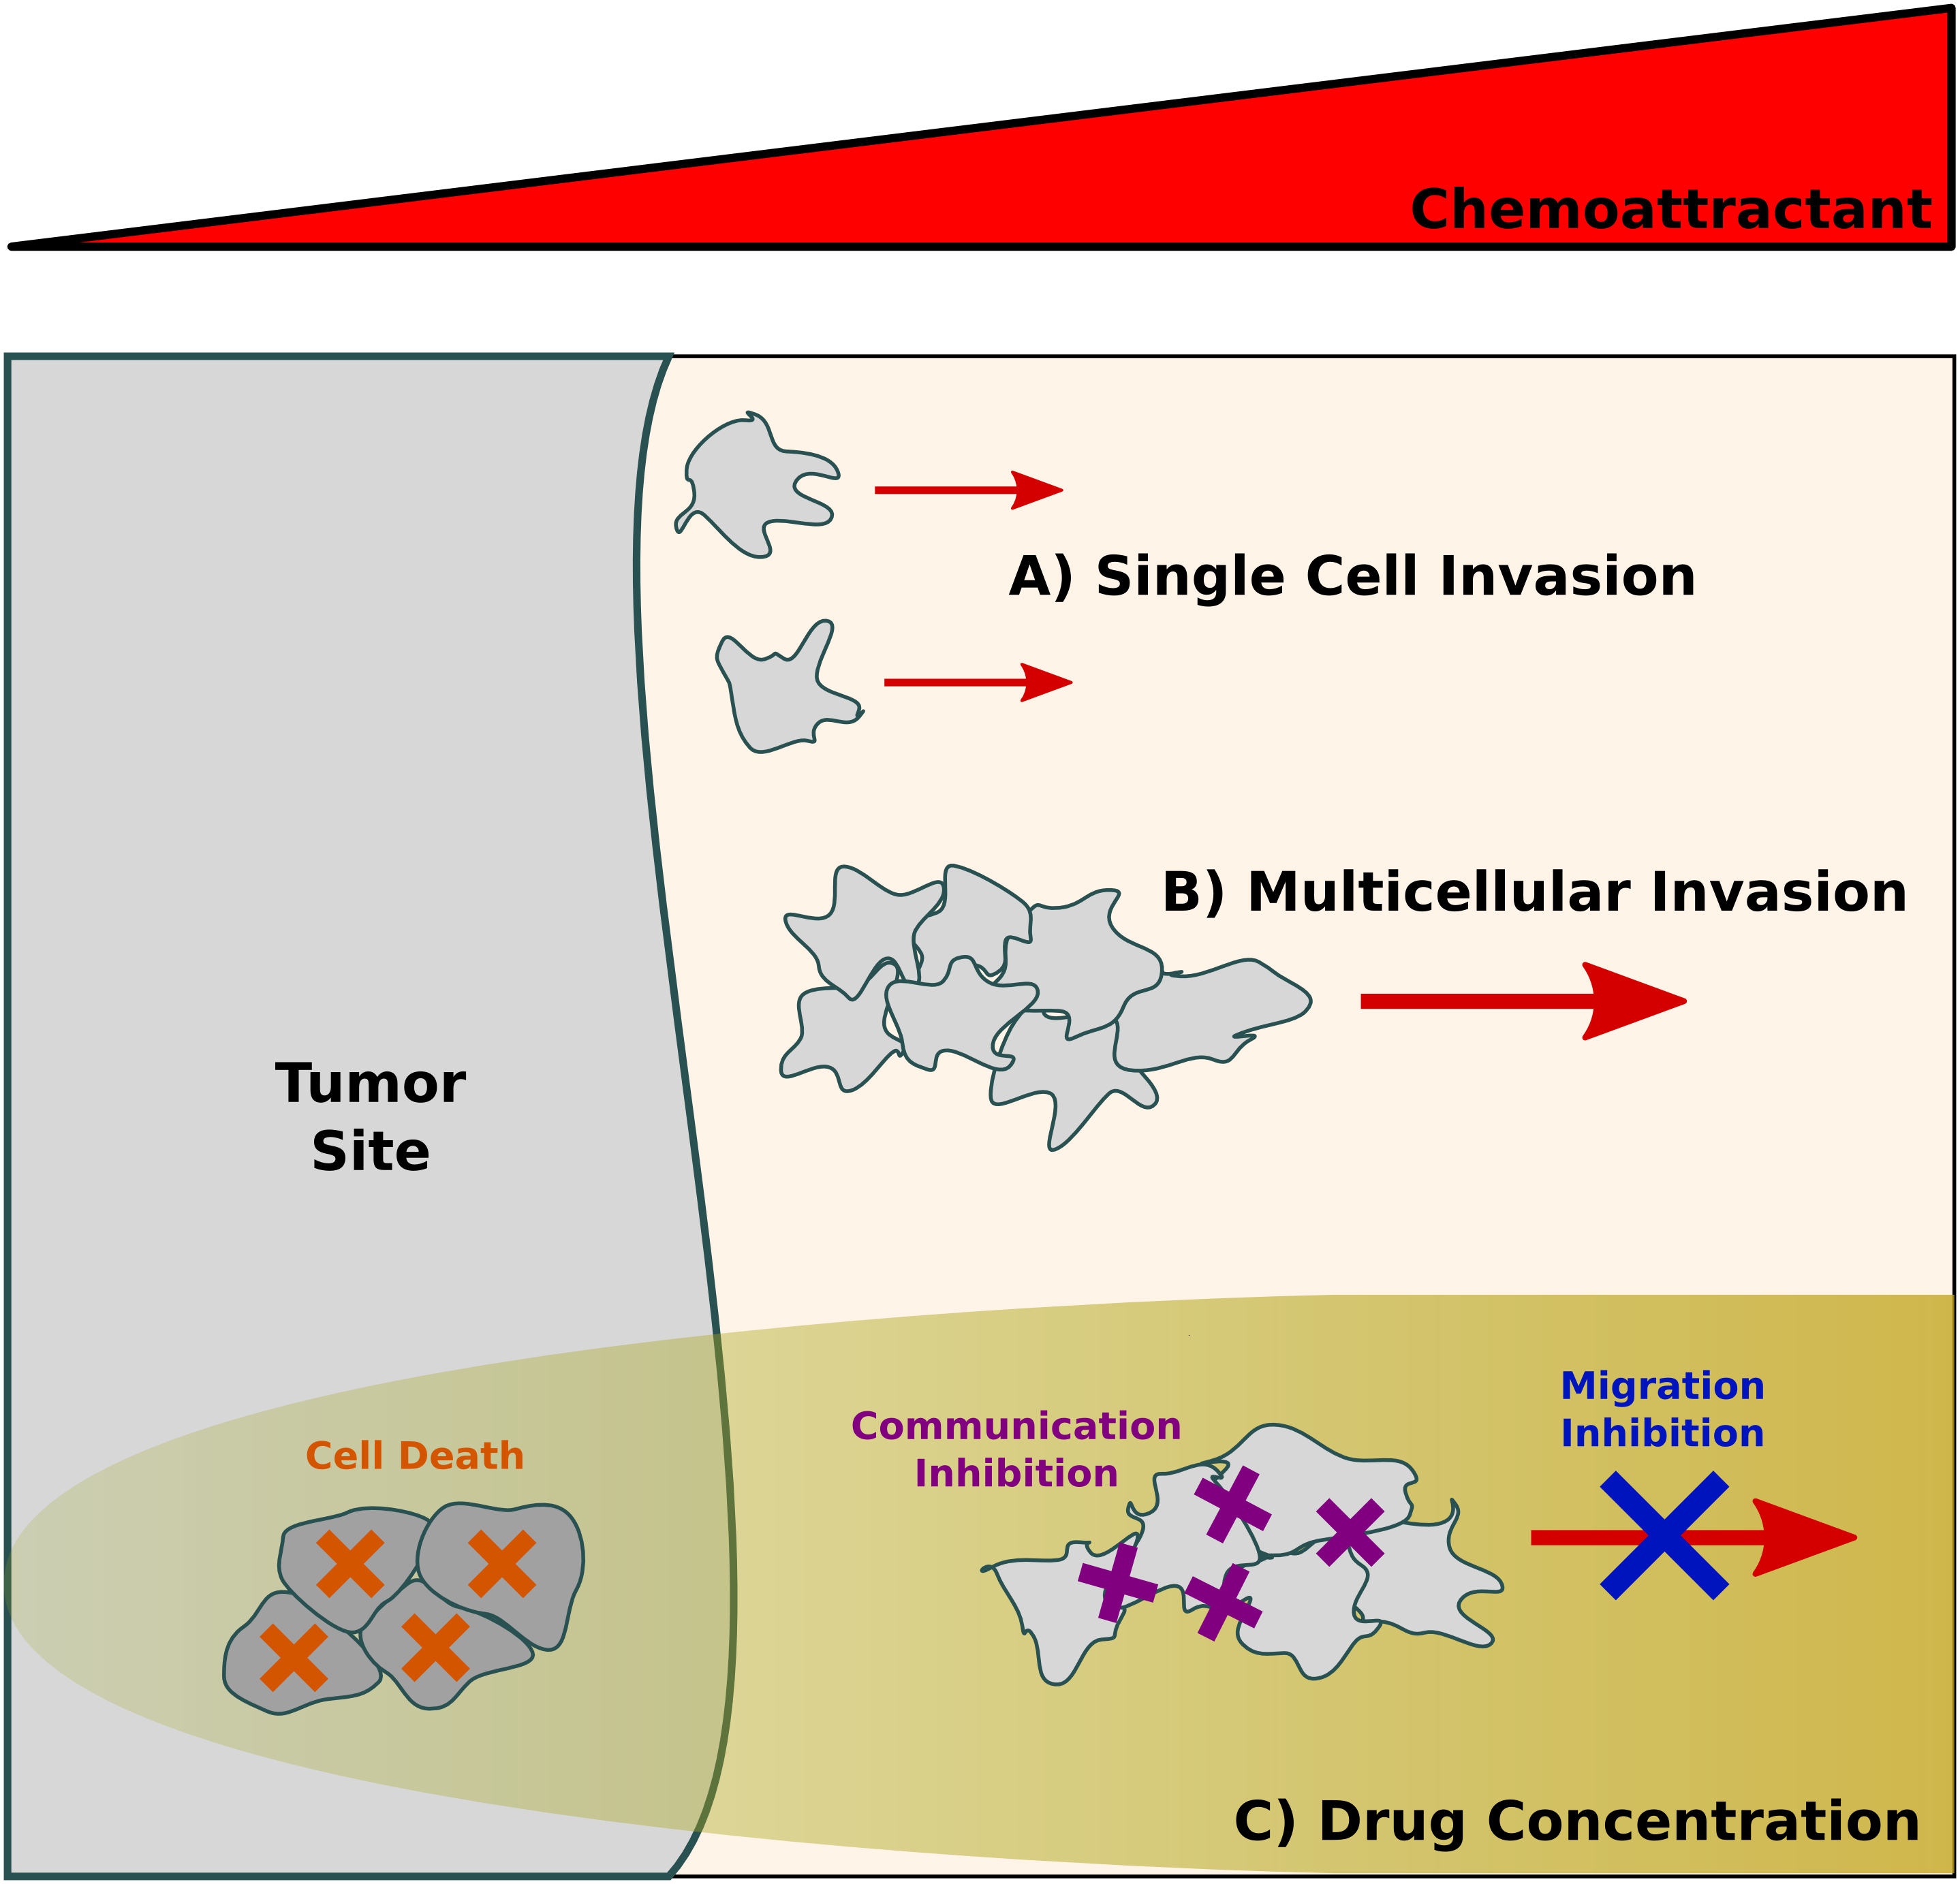
\includegraphics[width=0.8\textwidth]{../fig/ch1_fig1.png}
    \caption{Metastatic invasion is guided by chemical attractants and can occur via (A) single cells or (B) multicellular groups. (C) Drugs are delivered to the tumor environment in order to prevent tumor growth and metastasis. Drugs may cause cell death (orange), block cell-to-cell communication (purple), or prevent cell migration (blue).}
\label{fig:ch1_1}
\end{figure}


Furthermore, in many biological contexts cells act in close proximity to one another so their interactions may have a significant impact on their chemotactic performance \cite{theveneau2010collective}. During metastasis, chemotaxis can occur as a multicellular phenomenon involving the coherent motion of connected groups of cells (Fig.\ \ref{fig:ch1_1}B). In either the single-cell or multicellular case, the ability to precisely detect chemoattractants in the environment is bounded by the inherent diffusive fluctuations of the chemoattractants. Therefore it is important to understand the impact of diffusive noise on chemotactic precision.

In order to address the open question regarding how gradient sensing is linked to chemotactic performance we develop a framework of chemotaxis models. These theoretical and computational models
link sensing to polarization in order to examine how extrinsic noise from cell sensing puts physical constraints on chemotaxis. Starting in the following section, we briefly review the fundamental limits to concentration sensing and gradient sensing precision for single cells and multicellular collectives.
We also review how sensitive cells and collectives are to chemical signals and highlight how collective effects can enhance sensory response.
In Sect.\ 1.2 we review methods for modelling cell motion in relation to chemotaxis which will act as a foundation for the computational models developed in the proceeding chapters.

In Ch.\ 2 we review the physical limits to sensory precision, and discuss different chemotaxis modeling techniques.
Starting with Ch.\ 3, we apply computational and theoretical techniques to study human breast cancer cell chemotaxis. Computational simulations are conducted to explain and predict breast cancer cell chemotactic performance, and provide a relationship to common cell-migration experimental observables. We find that our simulations and theoretical model place physical constraints on the chemotactic performance of the cells observed in experiments. Single-cell chemotaxis simulations also give predictive power over how experimental parameters affect chemotactic performance in different ways.
Next, in Ch.\ 4 we examine multicellular chemotaxis. Cells very often exist and function in collective groups and chemotaxis is no different. We develop a novel theoretical approach to studying the effects of extrinsic noise on collective chemotaxis. We find that chemotactic performance is dependent on the type of collective behavior as well as on experimental parameters.
In Ch.\ 5 we extend our single-cell chemotaxis simulations to multicellular chemotaxis. We developed a model that explicitly accounts for the extrinsic noise in the diffusing chemoattractant concentration, as well as noise in intercellular communication in order to study the performance of communication-aided multicellular chemotaxis.
Finally, in Ch.\ 6 we summarize the models and results presented in the thesis.



\chapter{Constraints on Single-Cell Chemotactic Performance}

\noindent
In this chapter we examine the constraints that the external environment poses on single-cell chemotaxis. The work presented here is the product of a collaborative project with Dr.\ Bumsoo Han's group at Purdue University. In conjuction with Dr.\ Han and Hye-ran Moon's experiments on human breast cancer cell chemotaxis, I developed a computational model of single-cell chemotaxis. From simulations we are able to predict how environmental parameters affect breast cancer cell chemotactic performance. Additionally, We use a simple random walk model of chemotaxis to validate simulation results. The analytical model explains how environmental parameters constrain chemotactic performance, and predict limits to chemotactic accuracy and persistence.

As mentioned in Chapter 1, chemotaxis can be broken down into cell sensing, polarization, and locomotion. How well the cell executes these aspects of chemotaxis determines its performance. Just as the fundamental limits to cell sensory precision are set by the extrinsic noise in chemical diffusion, chemotactic performance is limited by extrinsic and intrinsic parameters comprising its three core components. The ability for the cell to polarize and induce motility is an intrinsic property of the particular cell-type in question, whereas environmental parameters affect what the cell can sense and its ability to migrate. Environmental parameters extrinsically constrain chemotaxis because they are independent of cell-type. Using our experimental data we can fit cell-dependent simulation parameters from observed results, allowing us the freedom to vary environment-dependent parameters. Here we focus solely on environmental parameters since they are independent of cell-type, and study how they place extrinsic limits on chemotactic performance.

Before presenting experimental, simulation, and analytical results, the most prevalent chemotaxis metrics found in the literature are reviewed. This is important because a wide variety of metrics are used to measure the chemotactic performance. Different metrics may be used to characterize one aspect of chmeotaxis, and several metrics go by the same or very similar names. All metrics are dependent on the details of each experimental set-up to varying extents, and it is frequently unclear how different metrics can be compared or related between studies. This ambiguity makes identifying quantitative patterns between different studies very challenging. Effective chemotaxis crucially depends on adequate accuracy, persistence, and speed in cell dynamics. From the review three metrics are identified that provide a comprehensive and intuitive description of chemotactic behavior.

With metrics for accuracy, persistence, and speed identified, we present the results from the breast cancer cell chemotaxis experiments. Simulations of single-cell chemotaxis probe beyond what is experimentally feasible, and identify the characteristic effects environmental parameters have on chemotactic performance. Finally, a simple analytical model is used to determine the extrinsic limits on cell chemotactic accuracy and persistence. Using experimental data we can fix the cell dependent parameters of the analytical model and predict a constrained phase-space in chemotactic accuracy and precision.

\begin{figure}
    \centering
    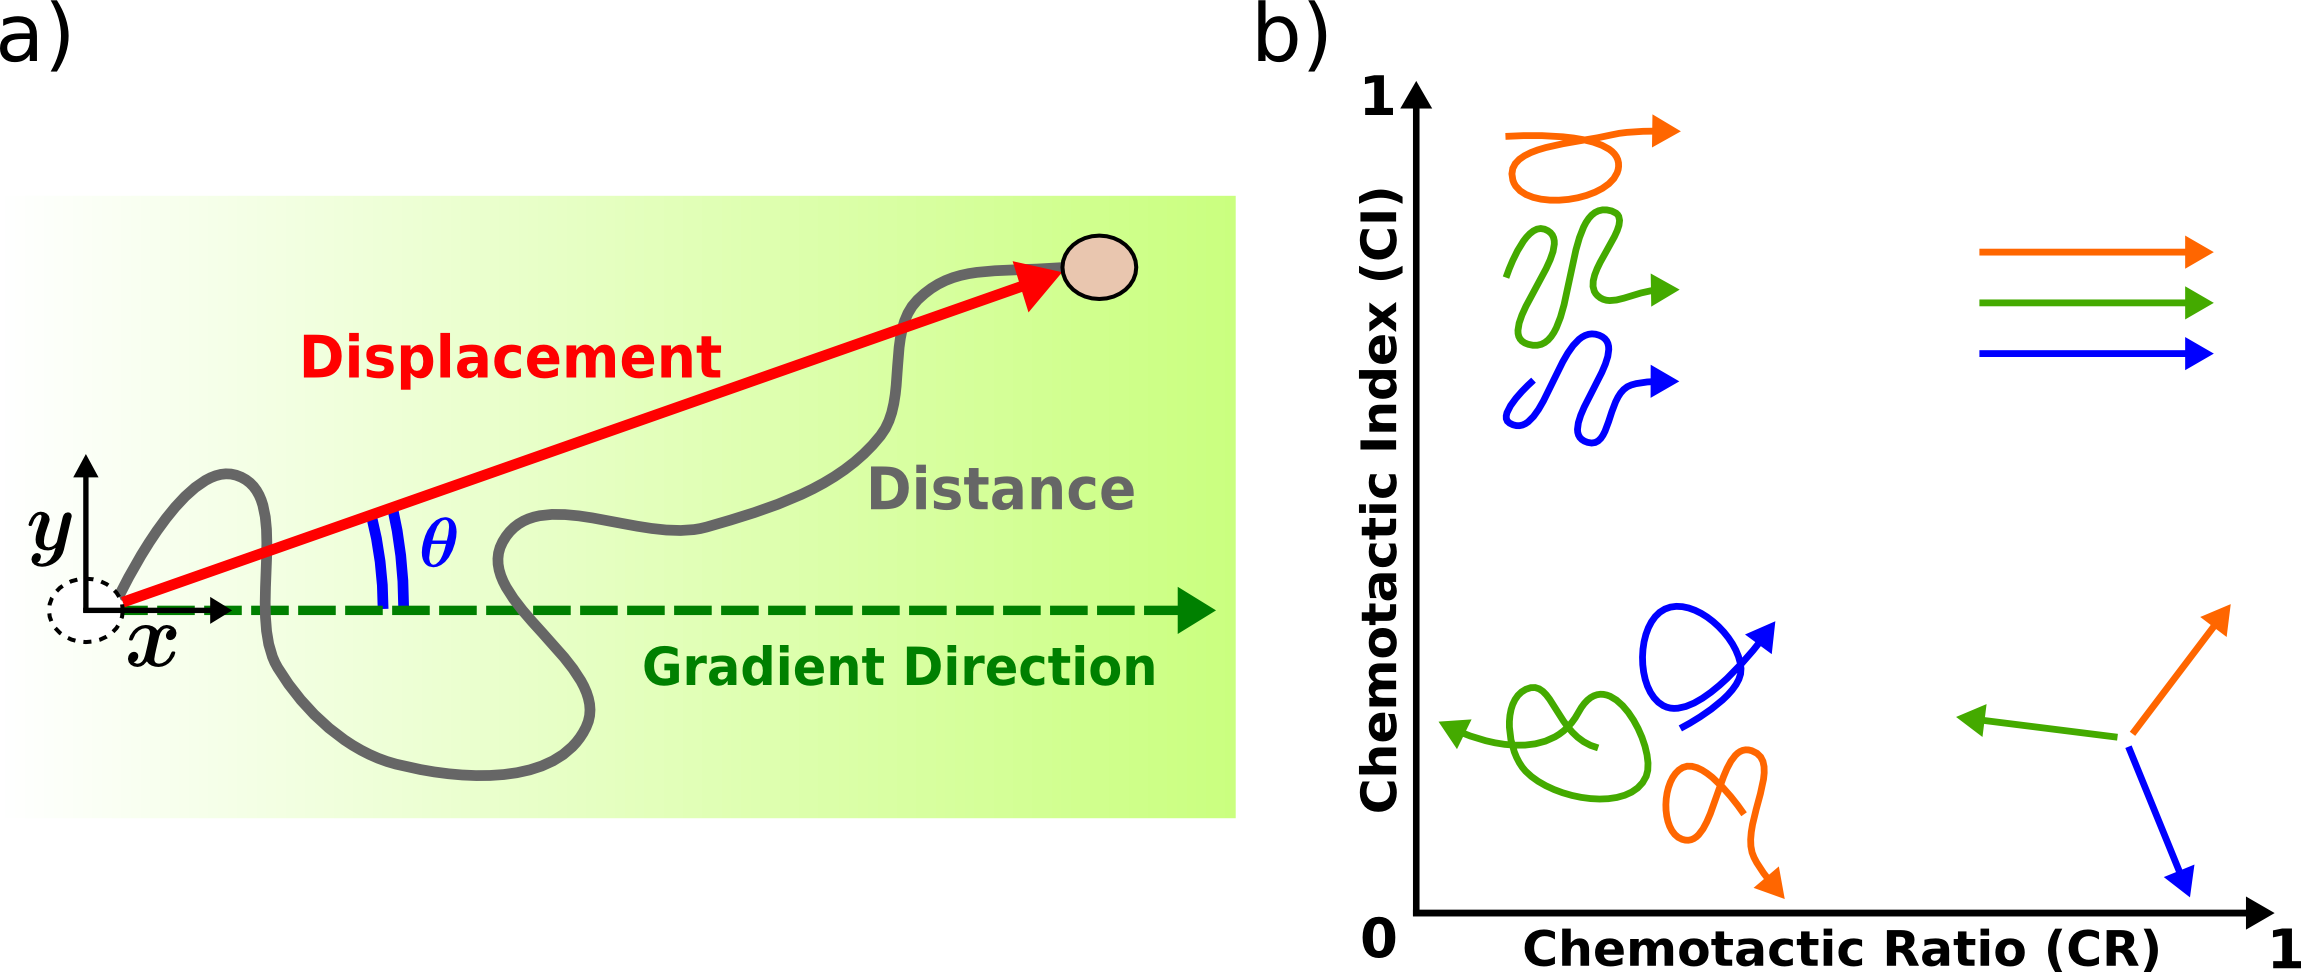
\includegraphics[width=0.90\textwidth]{../fig/ch2_fig1.png}
    \caption{a) Illustration of cell chemotaxis. The cell's displacement makes an angle $\theta$ with the gradient direction. b) Illustration of cell trajectories associated with different CI and CR values. Illustrations of typical cell trajectories are shown in different colors.} \label{fig:ch2_1}
\end{figure}


\section{Review of Chemotaxis Metrics}

The literature on cell migration and chemotaxis experiments contains a variety of different metrics used to characterize cell motion. In this section we briefly review some of the more common metrics used for measuring cell motility, persistence (also referred to as directionality) and chemotactic performance. Common metrics from the literature and their definitions are explained in order to motivate the metrics used in our study.

\subsection{Accuracy}

For chemotaxis experiments, often a single metric typically referred to as the chemotactic index is reported to quantify how well cells track the chemoattractant in question. However, the mathematical definition of the chemotactic index (CI) varies throughout the literature, the most common definitions are listed. CI has been defined as the ratio of the distance traveled towards the chemoattractant to the distance traveled in the absence of chemoattractant \cite{nelson1975chemotaxis}, the ratio of the number of cells that migrate in response to a chemical to the number of cells that migrate in the absence of stimulus \cite{iellem2001unique,mayr2002vascular,fiedler2005vegf}, and the population average of the cosine of the angle made between a cell's displacement and the gradient direction
\cite{funamoto2001role,mouneimne2006spatial,van2007biased,kay2008changing}.

The former two ratio-based definitions are commonly found in the literature although comparing them between different experiments is difficult. Both definitions give a measure of the migratory response when cells are exposed to a certain chemical. They may confound the effects of chemokinesis and chemotaxis since the former induces cell motility but not necessarily directed migration. Exposure to a motility inducing chemical will increase the response the cells have and thereby increasing CI, although cellular response may not be directed. Furthermore, neither definition clearly characterizes the cell's accuracy in tracking the chemoattractant; instead they quantify a fraction of cells that respond to the chemical and this does not capture any information about the cells' directedness. In the case of these two metrics $\text{CI} = 1$ corresponds to no chemotactic response and $\text{CI} > 1$ represents an increased response. Since CI here is unbounded, getting physical intuition for various values that are greater than one is difficult.

In this study we use the definition based on cosine of the angle cell trajectories make with the chemoattractant gradient direction as illustrated in Fig.\ \ref{fig:ch2_1}a. Specifically, we define CI as the population average of the cosine of the angle made between a cell's displacement and the gradient direction \cite{mouneimne2006spatial,kay2008changing,funamoto2001role},
\begin{equation} \label{eq:defCI}
    \text{CI} \equiv \langle \cos \theta \rangle \ .
\end{equation}
Strictly speaking, CI is bounded between -1 and 1, but for chemotaxis in response to a chemoattractant -- as is the case in this study -- CI generally falls between 0 and 1. $\text{CI} = 1$ represents perfectly accurate chemotaxis in which cell displacement is parallel to the gradient direction (Fig.\ \ref{fig:ch2_1}b, top-half), and $\text{CI} = 0$ indicates that the cells' migration is unbiased (Fig.\ \ref{fig:ch2_1}b, bottom-half). Having a bounded metrics makes it easy to compare different values of CI and get an intuitive picture for the type of cell dynamics it represents. The bounded nature of Eq.\ \ref{eq:defCI} along with its clear characterization of accuracy make it superior to the ratio-based definitions of CI, and this metric is also more easily comparable between experiments.

\subsection{Persistence}

Cell migratory persistence is commonly quantified using the chemotactic ratio and the directional autocorrelation function. The chemotactic ratio (CR) is defined as the ratio of the cell's displacement to the total distance traveled (Fig.\ \ref{fig:ch2_1}a):
\begin{equation} \label{eq:defCR}
    \text{CR} \equiv  \left\langle \frac{\text{displacement}}{\text{distance}} \right\rangle \ .
\end{equation}
The CR metric goes by several names in the literature such as the McCutcheon index \cite{mccutcheon1946chemotaxis}, directionality (ratio), length ratio \cite{gorelik2014quantitative}, and straightness index \cite{codling2008random}.
CR is dimensionless, bounded between 0 and 1 and intuitive sense can be made of either limit. If $\text{CR} = 1$, then the cells are moving in perfectly straight lines and motion is optimally efficient (Fig.\ \ref{fig:ch2_1}b, right-half). However, $\text{CR} = 0$ represents cell motion that is neither persistent nor efficient (Fig.\ \ref{fig:ch2_1}b, left-half), and it can be thought of as a cell trajectory that starts and ends at the same location.

The directional autocorrelation function (AC) calculates on average, how much time must pass for the cell's current direction of motion to be independent from the direction it was going in during the past \cite{gorelik2014quantitative,dang2013inhibitory}.
It quantifies persistence by calculating the timescale of decay in correlations between current and previous directions of motion.
The AC is defined as
\begin{equation} \label{eq:AC1}
    \text{AC}(\Delta t) = \langle \cos(\theta_{\Delta t + t}-\theta_{t}) \rangle_{t,N} \ ,
\end{equation}
with $\Delta t$ the time difference between two points in a trajectory and the average in Eq.\ \ref{eq:AC1} is taken over all starting times $t$ and all $N$ cell trajectories. The AC measures how the direction of cell motion along one trajectory is correlated with the direction of motion at a time $\Delta t$ later.
At $\Delta t = 0$, $\text{AC}(0) = 1$ since when no time has passed both angles in Eq.\ \ref{eq:AC1} are in fact the same. In the opposite limit, when a very large amoint of time has passed
$\text{AC}(\Delta t \to \infty) = 0$,
since trajectories that occurred infinitely far apart in time have no effect on each other. Calculating AC for all $\Delta t$ times sets a timescale $\tau$ which quantifies the rate at which correlations decay from 1 to 0. Therefore $\tau$ quantifies the persistence in the cells motion, a larger $\tau$ is indicative of more persistent motion. We define $\tau$ as
\begin{equation} \label{eq:tau1}
    \tau = \int_0^\infty dt' \ \text{AC}(t') \ .
\end{equation}
The AC is useful for cross-comparing experiments since the persistence timescale $\tau$ is largely independent of the frequency at which measurements were taken as well as the total observation time, unlike the CR. However, the timescale $\tau$ obtained from the AC is not a bounded dimensionless quantity unlike CR. For this reason we choose to use CR as the persistence metric over AC, and we discuss the validity of this choice after presenting the experimental results in Sect.\ 2.2.

% \begin{figure}[ht]
%     \centering
%     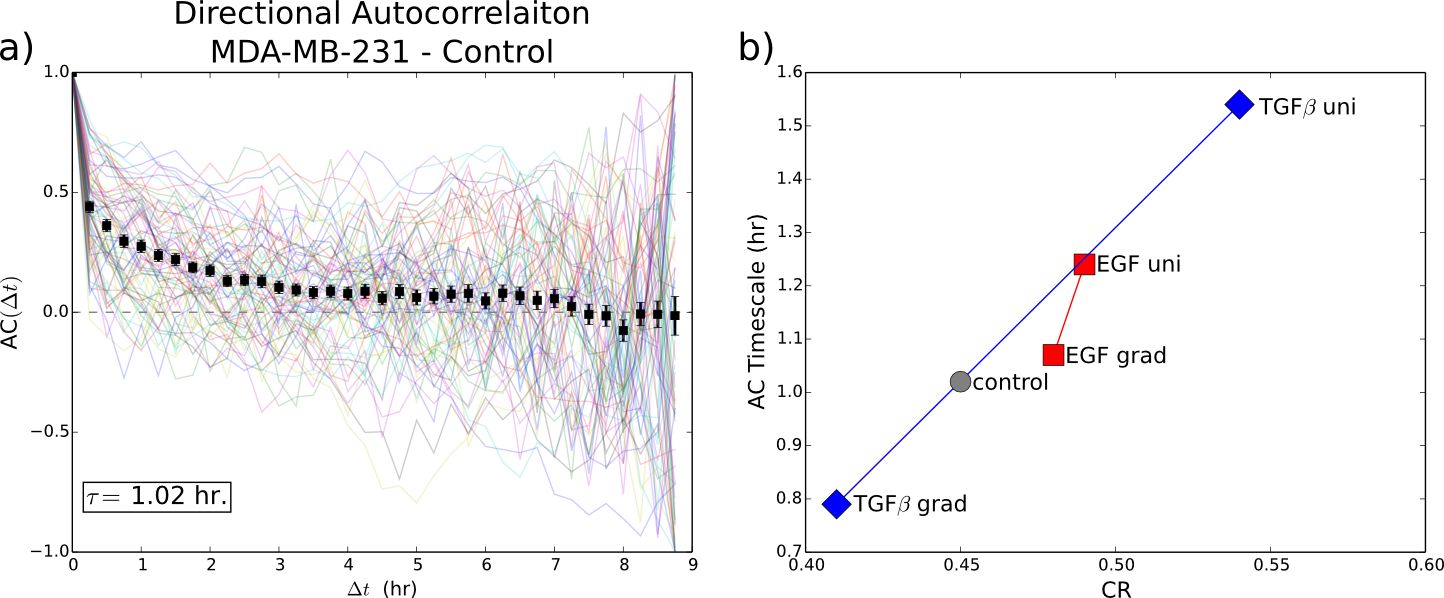
\includegraphics[width=0.80\textwidth]{../fig/ch2_fig5.png}
%     \caption{a) Directional Autocorrelation from control dataset. Light-colored trajectories indicate autocorrelations for individual cell trajectories. Timescale $\tau$ is calculated using Eq.\ \ref{eq:tau1}. b) Directional autocorrelation timescales and CR values for all experimental assays. Data points are color-coded based on chemical environment.} \label{fig:ch2_5}
% \end{figure}
%
% We calculate the AC and its timescale $\tau$ from our experimental data. Fig.\ \ref{fig:ch2_5}a shows the autocorrelations from the control assay, the black dots are the AC values for all times $\Delta t$ observed in our experiment, and its AC has a timescale
% $\tau = 1.02 \ \text{hr}$.
% In Fig.\ \ref{fig:ch2_5}b we compare the CR and AC timescale values from all experimental conditions. Going from a uniform to a graded concentration of either EGF or TGF$\beta$ results in a decreased CR value, and the AC timescale also decreases when going from a uniform to a graded concentration. This indicates that there is a monotonic relationship between CR and $\tau$. As the measured value of CR increases so too will the AC timescale $\tau$.
%
% Therefore, quantifying persistence with CR leads to the same patterns and analysis that could have been deduced from using AC. Additionally, the timescale obtained from the AC is not a bounded, dimensionless quantity. This makes gaining intuition about persistence from the autocorrelation timescale more difficult than CR. Since CR provides a clearer intuitive picture for persistence in cell chemotaxis we use it in our study.

\subsection{Migration Speed}

The final factor contributing to chemotactic performance is cell speed. Speed is important in order to ensure that the cells reach their destination in a timely manner. Cell speed is affected by many environmental factors such as collagen stiffness, and chemical concentration profiles. We define speed as the population average of the instantaneous cell speed during chemotaxis
\begin{equation}
    \bar{v} \equiv \left\langle \frac{||\Delta\vec{r}||}{\Delta t} \right\rangle \ ,
\end{equation}
with $\Delta t$ being the time lapsed between observations, and $||\Delta\vec{r}||$ the cell's displacement during that time period.
Experimentally, measuring cell speed is limited by the frequency at which cell trajectories are recorded. Therefore comparison of cell speed recorded in different chemotaxis studies necessitates careful consideration of the procedures used in each respective study. Nonetheless, speed is a simple, easily digestible metric for quantifying how motile cells are during chemotaxis.


\section{Experimental Results}

\begin{figure}
    \centering
    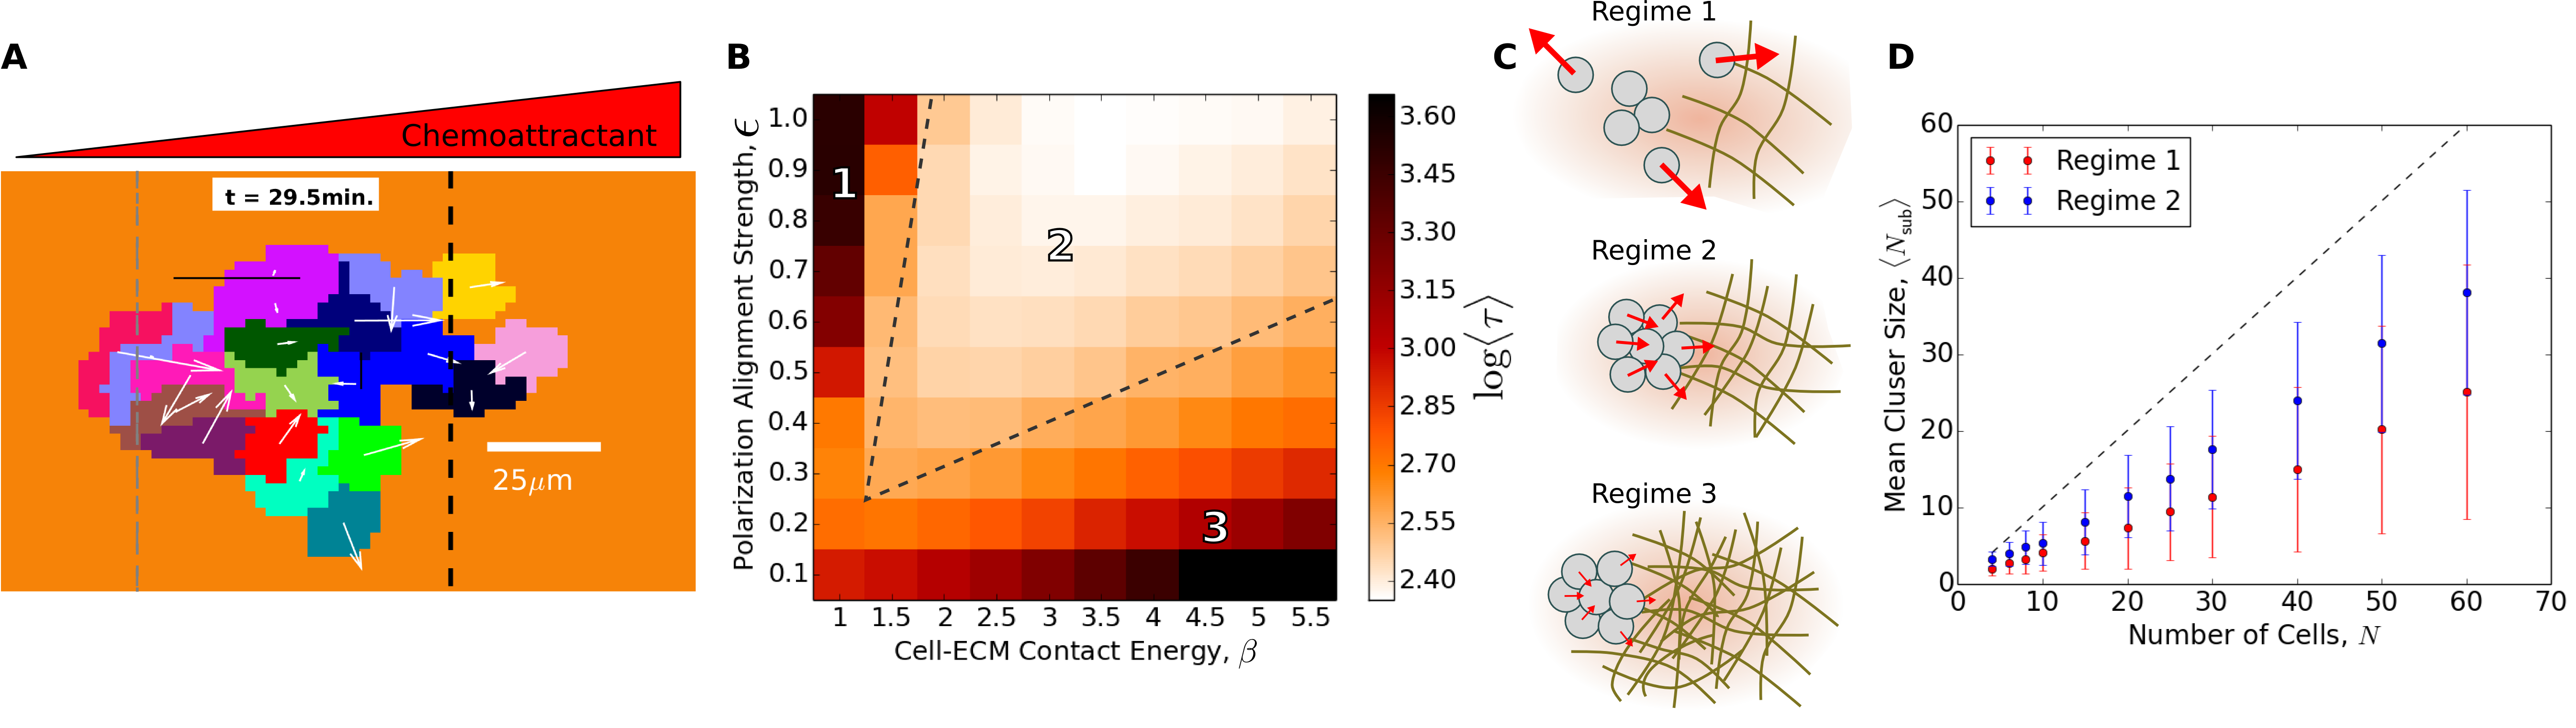
\includegraphics[width=0.90\textwidth]{../fig/ch2_fig2.png}
    \caption{Human breast cancer MDA-MB-231 cell chemotaxis assays. Cells are cultured in different chemical environments and trajectories are tracked. CI (a), CR (b) and mean speed ($\bar{v}$) are reported. d) Summary of chemotaxis assay results, data point size is proportional to mean speed. In all plots colors: no chemoattractant (gray), 400nM EGF uniform concentration (red), 0-800nM EGF gradient (orange), 25nM TGF$\beta$ uniform concentration (blue), and 0-50nM TGF$\beta$ gradient (light blue). Error bars are the standard error over the population of trajectories observed.} \label{fig:ch2_2}
\end{figure}

The Han group conducted experiments to measure the effects that the environment imposes on cell chemotaxis. Different chemicals known to induce motility and directed migration were used to measure how chemotactic performance would change. Human breast cancer cell line MDA-MB-231 was used in several different chemotaxis and motility assays.

Experiments were conducted in a soft lithography fabricated microfluidic device. The device contains three channels, two side channels and a center channel. Side channels are connected to reservoirs in order to control the chemical profile present in the center channel. The center channel consists of a collagen gel in which MDA-MB-231 cells are placed. The cells are surrounded by collagen and so perform three dimensional migration. The cells are cultured in the collagen for 48 hours followed by a 24 hour serum starvation period. Afterwards, concentrations of the chemoattractant of interest are added to the side channels. The concentration differences between the side channels creates a gradient through the collagen gel in the center channel. With the chemoattractant added to the device, images of the cells are taken every 15 minutes for a total duration of 9 hours in order to obtain single-cell chemotaxis trajectories. \r{Add a figure of experimental device / set-up.}

First, a control experiment was conducted to characterize the baseline behavior of the MDA-MB-231 cells (Fig.\ \ref{fig:ch2_2}, gray bars). As expected, when the cells are not in the presence of a chemoattractant they do not migrate in any preferred direction as indicated by a chemotactic index centered around zero (Fig.\ \ref{fig:ch2_2}a). However, even in the absence of any chemical signal cells do exhibit persistent motion with a $\text{CR} > 0$ (Fig.\ \ref{fig:ch2_2}b), since the cell motion is intrinsically directional due to the cells' internal migratory machinery \cite{petrie2009random}.
Similar persistent motion has been observed and modeled in the context of other cell types \cite{kim2013cooperative,codling2008random,othmer1988models}. Finally, we characterize the baseline cell motility, with a speed of $\approx 12 \mu\text{m/hr}$ (Fig.\ \ref{fig:ch2_2}c).

What happens when chemicals are added to the external environment? We start by performing assays with epidermal growth factor (EGF). EGF is a known motility inducing agent \cite{kim2013cooperative,mosadegh2008epidermal} and may also bias cell migration \cite{wang2004differential}. Experiments are conducted for both a uniform 400nM concentration and gradient of 0-800nM across.
As shown in Fig.\ \ref{fig:ch2_2}a, adding a uniform $400$nM concentration of EGF to the cellular environment results in a CI value within one standard error of $\text{CI} = 0$ indicative that the addition of EGF does not produce any significant bias to cell trajectories. This is expected since adding a uniform concentration of a chemical should not bias cell motion.
On the other hand, adding a graded EGF concentration profile does yield biased cell migration. With an average concentration of
$\bar{c}=400 \text{nM}$ and gradient of
$\bar{g}=0.80 \text{nM} / \mu\text{m}$
of EGF we find a CI value that is signficantly above zero (Fig.\ \ref{fig:ch2_2}a).
Examining the persistence and speed of cell movement (Fig.\ \ref{fig:ch2_2}b-c) shows that the uniform concentration gives similar results to the graded concentration. We observe that adding EGF results in about a 6\% increase in CR and an increased cell speed in agreement with the literature that EGF induces cell motility.

Next we used transforming growth factor type beta (TGF$\beta$) as a chemoattractant. TGF$\beta$ is a known chemoattractant for many cell types \cite{wahl1987transforming,bischoff1997chemotaxis}.
It is also involved in development, inflammation, and may be involved in carcinogenesis \cite{clark1998molecules,javelaud2004mammalian,pang2016tgf}.
Here we find that TGF$\beta$ is a strong chemoattractant (Fig.\ \ref{fig:ch2_2}a, light-blue) with $\text{CI} = 0.278 \pm 0.075$ when gradient of
$g = 0.05 \text{nM} / \mu\text{m}$ is used.
TGF$\beta$ does promote more directionally persistent motion as its CR value for a uniform concentration (but not for the graded concentration) is greater than that recorded for the control (Fig.\ \ref{fig:ch2_2}b). Adding TGF$\beta$ to the cellular environment does improve cell speed, but not to the extent that was observed for motility-inducing EGF (Fig.\ \ref{fig:ch2_2}c).

\begin{figure}[ht]
    \centering
    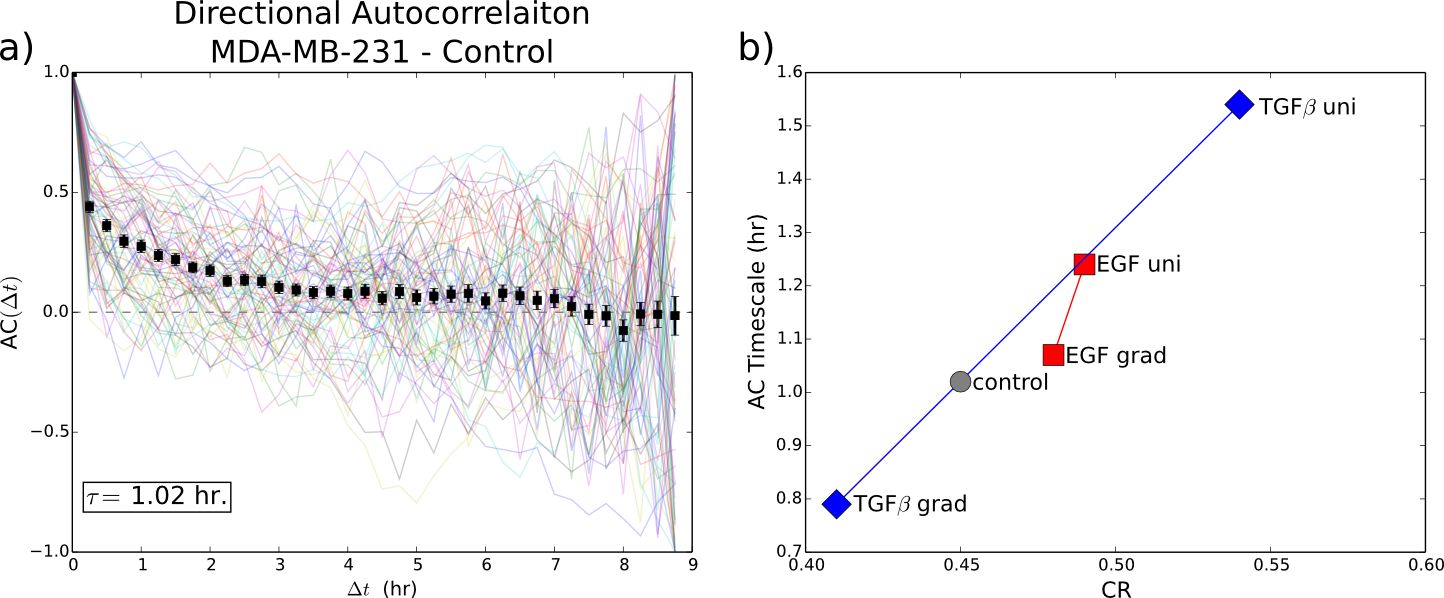
\includegraphics[width=0.80\textwidth]{../fig/ch2_fig5.png}
    \caption{a) Directional Autocorrelation from control dataset. Light-colored trajectories indicate autocorrelations for individual cell trajectories. Timescale $\tau$ is calculated using Eq.\ \ref{eq:tau1}. b) Directional autocorrelation timescales and CR values for all experimental assays. Data points are color-coded based on chemical environment.} \label{fig:ch2_5}
\end{figure}

For all experimental conditions we calculate the AC and its timescale $\tau$ in order to verify the validity in using the CR as the persistence metric instead of the AC timescale. Fig.\ \ref{fig:ch2_5}a shows the autocorrelations from the control assay, the black dots are the AC values for all times $\Delta t$ observed in our experiment, and its AC has a timescale
$\tau = 1.02 \ \text{hr}$.
In Fig.\ \ref{fig:ch2_5}b we compare the CR and AC timescale values from all experimental conditions. Going from a uniform to a graded concentration of either EGF or TGF$\beta$ results in a decreased CR value, and the AC timescale also decreases when going from a uniform to a graded concentration. This indicates that there is a monotonic relationship between CR and $\tau$. As the measured value of CR increases so too will the AC timescale $\tau$.
Therefore, quantifying persistence with CR leads to the same patterns, analysis, and conclusions that could have been deduced from using AC. Since CR provides a bounded dimensionless metric with clear intuition we use it instead of AC.

In summary, adding a gradient of EGF or TGF$\beta$ results in chemotaxis as indicated by CI values significantly above zero. The experimental parameter affects on chemotactic behavior are consolidated into Fig.\ \ref{fig:ch2_2}d. Movement in the CI-CR plane of Fig.\ \ref{fig:ch2_2}d indicates changing persistence and accuracy of chemotaxis, whereas the size of each data point represents the average speed. Under all conditions the cells move at speeds on the order of $\sim 10 \mu\text{m}/\text{hr}$. An increase in speed is observed when the MD-MB-231 cells are exposed to either growth factor. This is not not a surprising result since chemical agents that promote persistent or directed migration often results in increased motility \cite{petrie2009random}. EGF and TGF$\beta$ both produce similarly persistent motion though EGF promotes more motility as indicated by its fastest cell speed. In either case, the addition of the chemoattractant has more significant effect on chemotaxis accuracy than on its persistence.


\section{Chemotaxis Simulations}

The experiments tell us how cells respond to specific concentration profiles of EGF and TGF$\beta$. However, experiments do not tell us how chemotactic performance varies from experimental configuration to the next, and we are limited to testing conditions that experimentally feasible. Therefore we developed a computational model of chemotaxis in order to predict cell chemotactic performance in the presence chemical concentration profiles not yet experimentally tested.

Single cell chemotaxis simulations are also conducted to further probe cell chemotactic performance. With simulations environmental parameters such as collagen stiffness in addition to background chemical concentration and gradient can be easily varied over a wide range of values which may not be experimentally practical. These experimental parameters are individually varied to develop predictions on how each each parameter affects chemotactic accuracy (CI), persistence (CR), and speed.


\subsection{Computational Implementation}

\begin{figure}
    \centering
    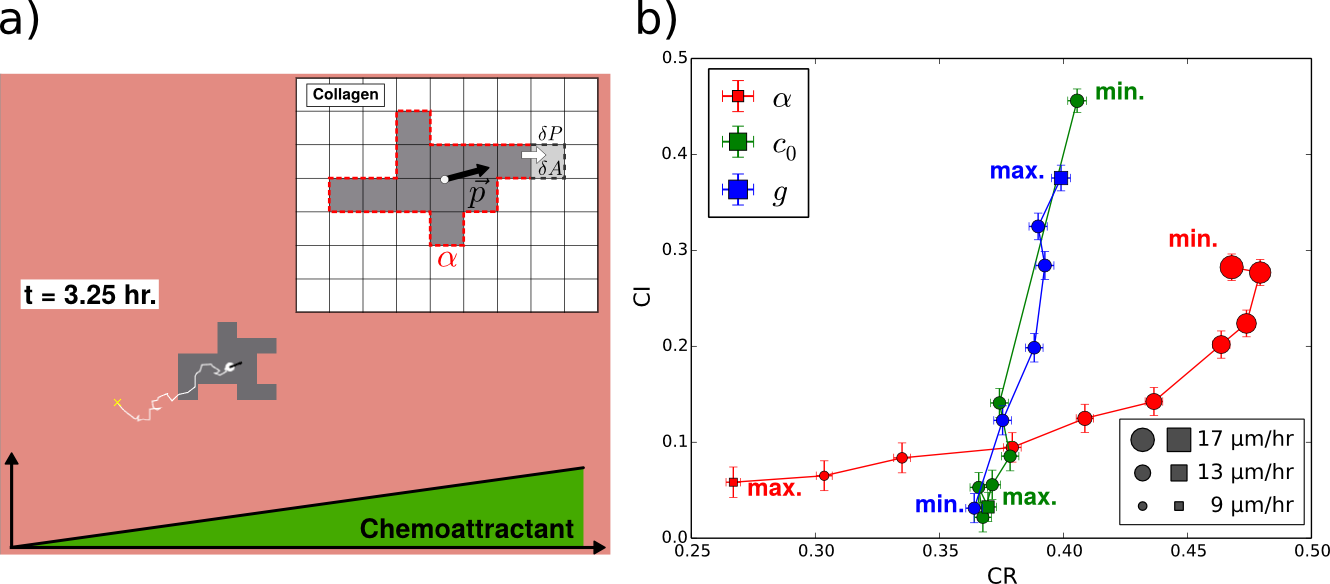
\includegraphics[width=0.80\textwidth]{../fig/ch2_fig3.png}
    \caption{a) Screen shot of simulation. Cell (gray) is migrating towards increasing chemical concentration, and the white line traces out the cell's path. Inset, illustration of the CPM. A Cell is comprised of simply connected lattice sites. There is an adhesion energy associated with cell-collagen contact, $\alpha$ (red-dashed line). Cell motility occurs through the addtion/removal of lattice sites (light-gray). The white dot represents the cell's center of mass and the black arrow its polarization vector $\vec{p}$. b) Simulation results. Environmental parameters collagen stiffness $\alpha$ (red), background concentration $c_0$ (green), and gradient $g$ are varied (blue).
    Parameter values along each trajectory: $\alpha \in \{ 0.1, 0.4, 0.7, 1.0 \}, c_0 \in \{ 1.0, 10.0, 100.0 \ \text{nM} \}, g \in \{ 1.0, 5.0, 10.0 \ \text{nM}/\mu\text{m} \}$.}
    \label{fig:ch2_3}
\end{figure}

Cell chemotaxis simulations are implemented using the Cellular Potts Model (CPM) \cite{graner1992simulation,swat2012multi}. The CPM is a lattice based simulation implementation. Cells comprise of lattice sites, and cells move and fluctuate in shape through the stochastic addition and removal of lattice sites. Cells are defined as a finite set of simply connected lattice sites
$\{ x \}$ (Fig.\ \ref{fig:ch2_3}a, inset).
Cell lattice sites are given the lattice label $\sigma(x)=1$ whereas the extracellular environment's lattices are labeled $\sigma(x)=0$. Cells have a desired size $A_0$ and perimeter $P_0$ from which they can fluctuate at an energetic cost, and cells adhere to their surrounding environment with an adhesion energy $\alpha$. The energy of the whole system is the sum of adhesion, area-restriction, and perimeter-restriction terms,
\begin{equation} \label{eq:CPMu1}
    u = \alpha P + \lambda_A(A_0 - A)^2 + \lambda_P(P_0 - P)^2 \ .
\end{equation}
In Eq.\ \ref{eq:CPMu1} $A$ is the cell area, and $P$ is the cell's perimeter. The parameters $\lambda_{A}$ and $\lambda_{P}$ are the area and perimeter restriction costs.

Cell motion is a consequence of minimizing the energy of the whole system. This stochastic process is sensitive to thermal fluctuations and is modeled using a Monte Carlo scheme. In a system of $n$ lattice sites, one \textit{Monte Carlo} time step (MC step) is composed of $n$ attempts to copy a random lattice site's label to a randomly chosen neighboring site. An attempt is accepted with probability $\mathcal{P}$, which depends on the change in the system's energy $\Delta u$ accrued in copying over the lattice label,
\begin{equation} \label{eq:ch2_prob}
    \mathcal{P} =
    \begin{cases}
        e^{-\left( \Delta u - w \right)} &\ \Delta u - w > 0 , \\
        1 &\ \Delta u - w \leq 0 .
    \end{cases}
\end{equation}
Here the bias term $w$ acts to bias cell motion in the direction of its polarization, and it is necessary in order for cells to exhibit directed motion \cite{szabo2010collective}.
The bias term is defined as
\begin{equation}
    w = \Delta\hat{x} \cdot \vec{p} \ ,
\end{equation}
with $\Delta\hat{x}$ the unit vector pointing in the change in the cell's center of mass caused by the proposed addition or removal of a lattice site, and $\vec{p}$ is the cell's polarization vector (Fig.\ \ref{fig:ch2_3}a, black arrow). The dot product acts to bias cell motion since movement that is parallel to the polarization vector will result in a more positive $w$ which in turn results in a higher acceptance probability (Eq.\ \ref{eq:ch2_prob}). Having a bias term along with a non-zero $\vec{p}$ allows for directed migration in the CPM.

After the $n$ random attempts of adding and removing lattice sites occurs during one MC step the cell updates its polarization vector. The time evolution of the cell's polarization vector is defined as
\begin{equation} \label{eq:CPMp1}
    \frac{d\vec{p}}{dt} = -r\vec{p} + \Delta\vec{x} + \epsilon \vec{q}\ .
\end{equation}
The first term in Eq.\ \ref{eq:CPMp1} results in exponential decay of the cell's current polarization at a rate $r$. $\Delta x$ is the cell's displacement during the last MC step and it enables persistence in cell motion because it reinforces $\vec{p}$ in the cell's direction of motion. The third term represents chemotaxis, with $\epsilon$ the bias strength and $\vec{q}$ an abstraction of the cell's internal gradient sensing network. We define $\vec{q}$ as
\begin{equation} \label{eq:CPMq1}
    \vec{q} = \frac{1}{N_P} \sum_{i=1}^{N_P} \frac{c_i-\bar{c}}{\bar{c}} \ \hat{r}_i \ ,
\end{equation}
with the sum taken over all $N_P$ lattice sites which comprise the perimeter of the cell. $\hat{r}_i$ is a unit vector that points radially outwards from the cell's center of mass to the location of lattice site $i$. $c_i$ is the concentration of the chemoattractant sampled at the lattice site $i$ and $\bar{c}$ is the cell's measurement of the mean concentration in its local environment; $c_i$ is sampled from a Poisson distribution and $\bar{c}$ is the mean from all $c_i$ measured at each lattice site. If lattice sites along one edge of the cell measure concentrations that are higher than the average then $\vec{q}$ will point in that direction. Given a sufficiently large chemical gradient $\vec{q}$ will act to bias the cell's polarization $\vec{p}$ in the direction of the gradient.

The CPM used here is similar to that used in our previously published study on collective cell chemotaxis \cite{varennes2016collective}. The source code for the single-cell chemotaxis simulations can be found here \cite{ch2code}.

\subsection{Calibration of Simulation Parameters}

In order to be able to compare simulation results to experiments we must first calibrate the CPM parameters. The length and time scales of the simulation are set to the experimentally observed average cell size and speed over all assays. Internal cellular parameters, such as the cell polarization strength and decay rate, are then calibrated such that the simulation's CI and CR values are approximately the same as those observed in one experiment.

From experiments we know that cells are on average $400 \mu\text{m}^2$ in size, and we use this to set one lattice site to equal $5 \mu\text{m}$ such that cells occupy $\sim 10$ lattice sites. Next we calibrate the time-scale in simulations by equating the average cell velocity in simulations to approximately that observed experimentally, $\sim 10 \mu\text{m/hr}$. With this we equate a simulation time step to $5 \text{min}$. Finally, we need to calibrate the internal cell parameters. We consider internal cell parameters to be those which are not affected by the environment and are characteristic of the particular cell type we are simulating.
These include the energy costs of cell area and perimeter fluctuations $\lambda_A$, $\lambda_P$, the polarization decay rate $r$, and the bias strength $\epsilon$. These parameters are set such that the CI and CR found from simulations are approximately the same as that observed in experiment. With internal cell parameters fixed we may proceed to vary external parameters in order to predict chemotactic performance in these environments. External parameters are the collagen stiffness $\alpha$, background concentration $c_0$, and the concentration gradient $g$.


In running simulations internal parameters are fixed to the values used for the initial calibration. External parameters are varied in order to quantify their effects on chemotactic performance. The internal parameter values used as well as the baseline external parameter values are listed in Table \ref{table:ch2_1}.


\begin{table}[ht]
\begin{center}
\begin{tabular}{ |c|c|c| }
\hline
Parameter & Value & Notes \\ \hline
Relaxed Cell Area $A_0$ & $400 \ \mu\text{m}^2$ & \\ \hline
Relaxed Cell Perimeter $P_0$ & $3.6\sqrt{A_0} \ \mu\text{m}$ & Assumes circular resting shape \\ \hline
Area Energy Cost $\lambda_A$ & 0.3  & Prevents ``stringy'' cell-shapes \\
Perimeter Energy Cost $\lambda_P$ & 0.01 & \\ \hline
Polarization Bias Strength $\epsilon$ & 0.1 & \\ \hline
Polarization Decay Rate $r$ & $2.4 \ \text{hr}^{-1}$ & Sets polarization memory time \\ \hline \hline
Cell-environment Contact Energy $\alpha$ & 0.7 & Sets energy scale \\ \hline
Concentration $\bar{c}$ & $10 \ \text{nM}$ & \\
Gradient $g$ & $0.5 \ \text{nM/}\mu\text{m}$ & \\ \hline
\end{tabular}
\caption{Table of parameters and values used in simulations. The first six parameters are intrinsic to the cell and remain fixed. The final three parameters represent the environment and are varied in Fig.\ \ref{fig:ch2_3}. Energy costs are in units of $k_B T$, where $k_B T$ is the thermal energy of the CPM Monte Carlo scheme.}
\label{table:ch2_1}
\end{center}
\end{table}


\subsection{Simulation Results}

With length and time scales of the simulation are calibrated and internal cellular parameters fixed, we vary the external, environmental parameters.    Fig.\ \ref{fig:ch2_3}b shows the resulting CI, CR and speed values when environmental parameters are changed. Each data point along a parameter's trajectory indicates the CI and CR values, while the size of the data point indicates the average speed for that particular choice of parameter value. All other parameters are held fixed along each trajectory. The background concentration is varied over three orders of magnitude whereas both the gradient and collagen stiffness are varied over one order of magnitude.

We find that varying the background concentration and gradient most significantly affects the accuracy of chemotaxis, not the persistence nor the speed. This is displayed in Fig.\ \ref{fig:ch2_3}b in which both $c_0$ and $g$ have much longer trajectories along the CI axis than along either the speed or CR axis.
As the background concentration increases, the fluctuations in the diffusing chemoattractant become larger relative to the gradient making it more difficult for the cell to correctly determine the gradient direction. This results in a decreasing CI as $c_0$ increases. Conversely, increasing the gradient enables the cell to more accurately detect the gradient direction resulting in increasing CI values (Fig.\ \ref{fig:ch2_3}b,c).

Along with changing the accuracy of chemotaxis, varying $c_0$ and $g$ also results in slightly increased persistence and speed. This goes hand in hand with the improved gradient detection due to increased $g$ or decreased $c_0$. As cells become more accurate movements perpendicular to the gradient are reduced, resulting in more persistent and faster motion along the gradient direction as shown in Fig.\ \ref{fig:ch2_3}b.

Collagen stiffness is the only parameter that significantly affects the persistence in the cell's motion, indicated by the larger displacement in $\alpha$'s trajectory along CR versus CI or speed (Fig.\ \ref{fig:ch2_3}a,b). Stiffer collagen is more difficult for cells to traverse leading to slower speeds, and we find a monotonic relationship between CR and speed when stiffness is varied (Fig.\ \ref{fig:ch2_3}b). As was observed for the chemoattractant-related parameters the more persistent cell motion seen at small $\alpha$ also corresponds to more accurate, faster chemotaxis.

From these simulation results we deduce some stereotypical patterns of cell chemotaxis. Increasing the relative change in chemoattractant concentration across a cell length (either by increasing $g$ or reducing $c_0$) results in more accurate chemotaxis. Materials that are more difficult for cells to traverse during chemotaxis, whether its stiffer colagen \textit{in vitro} or denser extracellular matrix \textit{in vivo}, results in reduced chemotactic performance across all metrics. Finally, the simulations show a positive correlation between CR and speed since as cell motion becomes more persistent it typically enables faster cell movement.

\section{Analytical Model of Chemotaxis}

Interestingly, although both experiments and simulations vary environmental parameters affecting cell chemotaxis, the chemotactic performance metrics do not dramatically change. Both CI and CR can range from 0 to 1, but our MDA-MB 231 cell assays result in CR values close to 0.45 and CI values less than 0.3 for all environmental conditions (Fig.\ \ref{fig:ch2_2}). Simulations allow for probing chemotactic behavior over an even larger parameter space, and yet CI and CR values remain limited to a fraction of the whole range (Fig.\ \ref{fig:ch2_3}).

Can this phenomenon be explained with a simple physical model? One of the simplest models for cell movement and chemotaxis is the biased persistent random walk \cite{alt1980biased,othmer1988models}. In its simplest form, a random walk involves a walker that is equally likely to move in any direction, and its next movement is independent of its previous motion. To add persistence to the random walk means that the walkers' movements are correlated. The walker's next movement is not equally likely in all directions as in the simplest case, but now depends on its previous direction of motion \cite{patlak1953random}. Finally, adding bias means that the walker is more likely to move in a particular fixed direction.
Before we get into how the BPRW model can shed light on the chemotactic performance of MDA-MB-231 breast cancer cells, lets review the model formulation.

\subsection{Biased Persistent Random Walk Formulation}

The BPRW is modeled as a velocity jump process instead of the typical on lattice hopping formulation of the standard random walk. In the BPRW a walker moves in a particular direction with fixed speed for an exponentially distributed amount of time before changing direction. The walker reorients to a new direction $\hat{v}$ from its previous direction $\hat{v}'$ depending on the probability density $T(\vec{v},\vec{v}')$. We assume a reorientation frequency $\lambda$, thus $\lambda^{-1}$ is the average run time, and we assume that it moves at a constant speed $s$. The reorientations are chosen based on a probability density $T(\vec{v},\vec{v}')$ which depends only on the angular direction of the walker's movements: $T(\vec{v},\vec{v}') = T(\theta,\theta')$. Here the angle $\theta$ is taken relative to the $x$ axis which is assumed to be parallel to the gradient direction.

Let $p(\vec{r},\theta,t) d\vec{r} d\theta$ be the number density of individual walkers found between positions $\vec{r}$ and $\vec{r}+d\vec{r}$ with movement orientation between $\theta$ and $\theta + d\theta$. From Othmer \textit{et al}.\ \cite{othmer1988models} it is shown that the evolution equation for the probability density $p(\vec{r},\theta,t)$ simplifies to
\begin{equation} \label{eq:p1}
    \frac{\partial p}{\partial t} + s \vec{\xi}\cdot\vec{\nabla} p =
    -\lambda p + \lambda \int_{-\pi}^{\pi} d\theta' \ T(\theta,\theta') \ p(\vec{r},\theta,t) \ ,
\end{equation}
with $\vec{\xi} = (\cos\theta,\sin\theta)$. In order to derive expressions for the moments some assumptions have to made on the reorientation probability density. We assume that $T(\theta,\theta')$ is the sum of two functions,
\begin{equation} \label{eq:t1}
    T(\theta,\theta') = \underbrace{k(\theta)}_\text{bias}
    + \underbrace{h(\phi)}_\text{persistence}
\end{equation}
with $\phi = \theta - \theta'$ being the turning angle. $k(\theta)$ is maximally valued and symmetric about $\theta = 0$, and biases movement towards the gradient. $h(\phi)$ is the turning angle distribution which is assumed to be symmetric about $\phi = 0$. Along with these properties $T(\theta,\theta')$ and its component functions must obey the following conditions:
\begin{align} \label{eq:t2}
    &T(\theta,\theta') \geq 0 \ , \text{for all } (\theta,\theta') \ , \\
    \int_{-\pi}^{\pi} d\theta \ &T(\theta,\theta') = 1 \ , \label{eq:t3} \\
    \int_{-\pi}^{\pi} d\theta  \ &k(\theta)         = 0 \ , \label{eq:t4} \\
    \int_{-\pi}^{\pi} d\phi    \ &h(\phi)           = 1 \ . \label{eq:t5}
\end{align}

With Eq.\ \ref{eq:p1} and the restrictions on $T(\theta,\theta')$ (Eq.\ \ref{eq:t2}-\ref{eq:t5}), Othmer \textit{et al}.\ \cite{othmer1988models} derive the moments for the BPRW.
\begin{align} \label{eq:moment1}
    \begin{split}
    \langle r^2(t) \rangle &= \frac{2s^2}{\lambda_0} \left[ \left(1-\frac{2\chi^2}{(1-\psi)^2}\right)t
    - \frac{\chi^2 t e^{-\lambda_0 t}}{(1-\psi)^2}
    + \frac{3\chi^2(1-\psi)^{-2}-1}{\lambda_0} \left(1-e^{-\lambda_0 t}\right)
    \right. \\
    &\qquad \left.
    + \frac{\chi^2 \lambda_0 t^2}{2(1-\psi)^2} \right]
    \end{split} \\
    \langle x(t) \rangle &= \frac{\chi}{1-\psi} s \left(t -\frac{1-e^{-\lambda_0 t}}{\lambda_0} \right) \label{eq:moment2} \\
    \langle y(t) \rangle &= 0 \label{eq:moment3}
\end{align}
These results are derived with the assumption that individuals in the BPRW start at the origin with uniformly distributed initial orientations.
The mean squared displacement (Eq.\ \ref{eq:moment1}) and the mean walker location (Eq.\ \ref{eq:moment2}-\ref{eq:moment3}) both depend on the parameters $\chi$, $\psi$, and $\lambda_0$. The bias strength (also referred to as the taxis coefficient) is represented by $\chi$ which is defined as
\begin{equation} \label{eq:chi}
    \chi \equiv \int_{-\pi}^{\pi} d\theta \ k(\theta) \ \cos\theta \ .
\end{equation}
$\psi$ represents the persistence strength (also referred to as the persistence index), and it is defined as
\begin{equation} \label{eq:psi}
    \psi \equiv \int_{-\pi}^{\pi} d\phi \ h(\phi) \ \cos\phi \ .
\end{equation}
Note that the restrictions on the reorientation probability density (Eq.\ \ref{eq:t2}-\ref{eq:t5}) result in $\chi \leq 1 - \psi$. Fianlly, $\lambda_0$ is the effective turning rate of the walker,
$\lambda_0 \equiv \lambda(1-\psi)$.
Since $\lambda$ is the reorientation rate and $\psi$ is the persistence strength, $\lambda_0$ describes the effective rate at which the walker forgets its previous orientation.

Starting from the definitions for CI and CR in Eqs.\ \ref{eq:defCI}-\ref{eq:defCR}, we use the moments given in Eqs.\ \ref{eq:moment1}-\ref{eq:moment3} to calculate CI and CR for the BPRW model as functions of time:
\begin{align} \label{eq:ci1}
    \text{CI}(t) &= \left\langle \frac{x}{r} \right\rangle \approx
    \frac{\langle x \rangle}{\sqrt{\langle r^2 \rangle}}
    = \chi \sqrt{\frac{\lambda}{2(1-\psi)}} \left(t -\frac{1-e^{-\lambda_0 t}}{\lambda_0} \right) \
    [ \ \ldots \ ]^{-1/2} \ , \\
    \text{CR}(t) &= \frac{\langle r \rangle}{L} \approx
    \frac{\sqrt{\langle r^2 \rangle}}{st}
    = \frac{1}{t}\sqrt{\frac{2}{\lambda_0}} \
    [ \ \ldots \ ]^{1/2} \ .
    \label{eq:cr1}
\end{align}
The term $[ \ \ldots \ ]$ is shorthand for the bracketed term in Eq.\ \ref{eq:moment1}, and $L$ is the total path length. In Eq.\ \ref{eq:ci1} we approximate the two moments as being independent of one another, and in both Eqs.\ \ref{eq:ci1}-\ref{eq:cr1} we make the approximation that
$\langle x \rangle \approx \sqrt{\langle x^2 \rangle}$.
These approximations are in very good agreement the exact solutions of CI and CR times in which many reorientation events occur, $t \gg \lambda^{-1}$. Note that neither CI nor CR depend on the speed $s$, and assuming that $\chi < 1 - \psi$, to first order CR decays as $\text{CR} \sim t^{-1/2}$.

The BPRW predictions for CI and CR depend on how strongly persistence and bias affect the walker's movements. The timescales in the BRPW are calibrated to those of our experiments; total observation time $t = 9 \text{hr}$, the reorientation frequency
$\lambda = 4 \text{hr}^{-1}$), and we approximate the speed to be
$s = 15 \mu\text{m/hr}$. With the BPRW timescales calibrated we can proceed to vary $T(\theta,\theta')$ which in turn affects the bias strength $\chi$, and the persistence strength $\psi$.

\begin{figure}[ht]
    \centering
    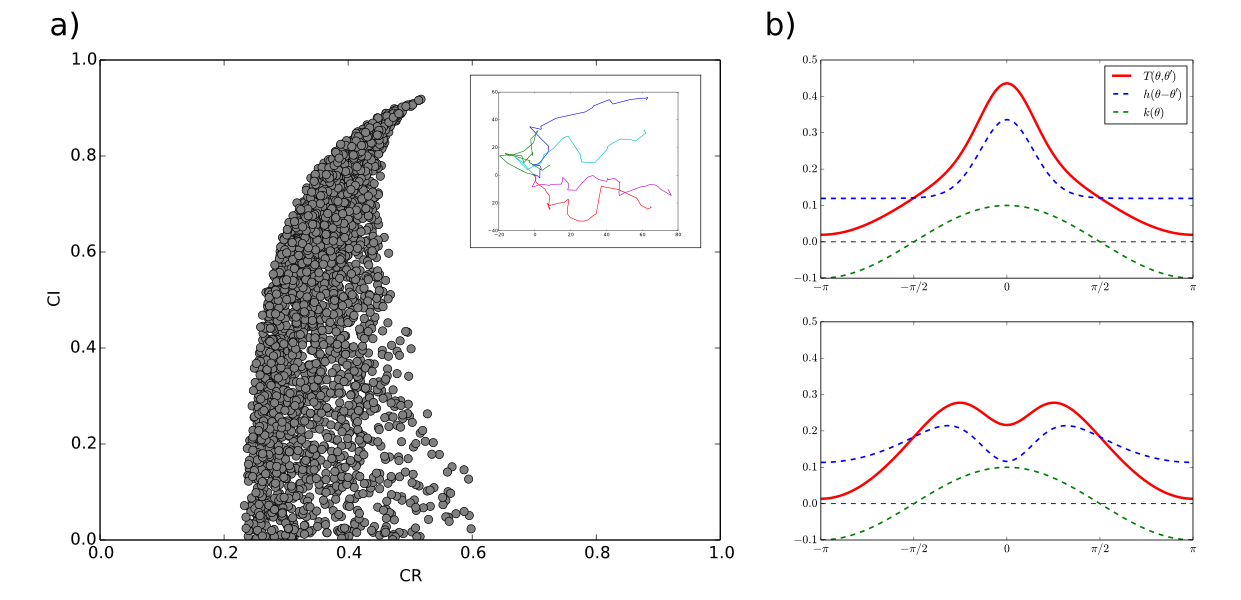
\includegraphics[width=0.80\textwidth]{../fig/ch2_fig6.png}
    \caption{a) Possible values of CI and CR for a BPRW. Each dot represents the CI and CR value for a BPRW of a given bias and persistence strength. Inset, sample trajectories of a BPRW. b) Example reorientation probability densities $T(\theta,\theta')$, and their component bias $k(\theta$) and persistence $h(\theta-\theta')$ functions. For both b) plots $\theta'=0$. For all plots: $t =36$, $\lambda = 1.0$, $s = 3.75$, and $\theta=0$ is the direction of bias.}
    \label{fig:ch2_6}
\end{figure}

Simulations of the BPRW are performed with varying $T(\theta,\theta')$ to find the resulting values of CI and CR possible given our experimental system. In the simulations the bias and persistence functions to take on the forms:
\begin{align}
    k(\theta) &= k_1 \cos\theta \ , \\
    h(\theta-\theta') &= h_1 f_\text{VM}(\theta | \ \theta', \kappa_1) + h_2 f_\text{VM}(\theta | \ \theta', \kappa_2) \ .
\end{align}
Here $k_1$ sets the bias strength, and $h(\theta-\theta')$ is a linear combination of two von Mises distributions with
$f_\text{VM}(\theta | \ \theta', \kappa) = \frac{1}{2\pi I_0(\kappa)} e^{\kappa \cos(\theta-\theta')}$.
The von Mises distribution is approximately equal to a normal distribution bounded to a circle, and it is commonly used in random walk models of biological systems \cite{codling2008random}.
The parameters $\kappa_1$ and $\kappa_2$ set the persistence strength with larger values of $\kappa$ resulting in higher persistence. $h_1$ and $h_2$ set the shape of the distribution, with $\{h_1,h_2\} > 0$ results in a single-peaked $h(\theta-\theta')$ function as shown in Fig.\ \ref{fig:ch2_6}b, top. Whereas, if $h_1> 0$ and $h_2<0$ then the resulting $h(\theta-\theta')$ function has two peaks, symmetric across $\theta=\theta'$ (Fig.\ \ref{fig:ch2_6}b, bottom).
Interestingly, even in this idealized model of chemotaxis the whole range of CI and CR values is not available to the BPRW. The mechanics of the random walk limit its performance resulting in behavior that cannot attain perfect accuracy ($\text{CI}=1$), nor perfect persistence ($\text{CR}=1$).

In summary, by calibrating BPRW to our experiments the parameters $t$, $\lambda$, and $s$ are fixed. From here we can sample possible CI and CR values given a particular bias and persistence strength. By varying over all possible combinations of bias and persistence parameters while enforcing the restrictions on $T(\theta,\theta')$ (Eq.\ \ref{eq:t2}-\ref{eq:t3}) all possible values of CI and CR permitted under the BPRW model are calculated. The CI and CR values permitted by our theoretical model are shown alongside the experimental results in  Fig.\ \ref{fig:ch2_4}. We see that our simple analytical model is able to recover the CI and CR values observed. More importantly, the BPRW puts limits on how well these breast cancer cells can chemotaxis regardless of how favorable the environmental conditions are made as represented by the gray-shaded region in Fig.\ \ref{fig:ch2_4}.

\begin{figure}
    \centering
    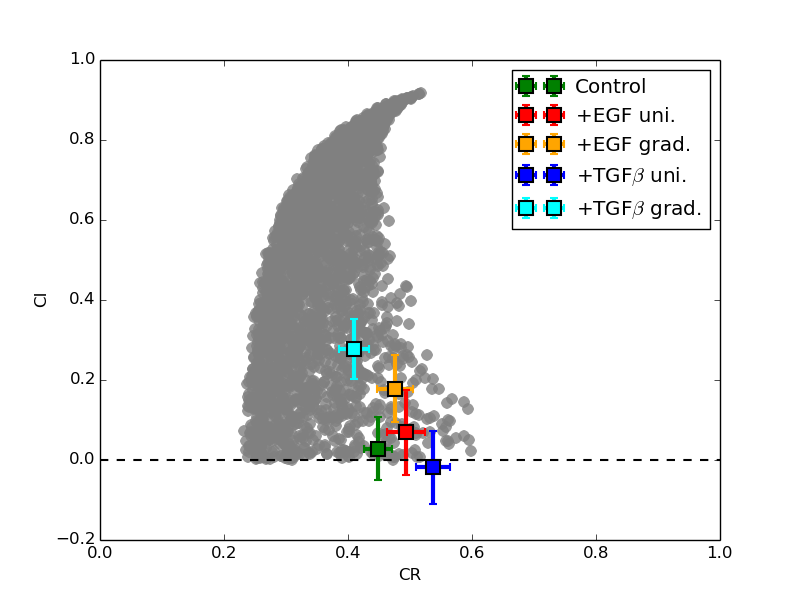
\includegraphics[width=0.80\textwidth]{../fig/ch2_fig4.png}
    \caption{Theoretical bounds on chemotactic performance based on the biased persistent random walk model. Gray dots represent possible theoretical CI and CR values for a BPRW. Colored squares are experimentally recorded values for different environmental conditions.} \label{fig:ch2_4}
\end{figure}



\chapter{Limits to Collective Chemotaxis}

\noindent
In this chapter we transition from studying single-cell chemotaxis to that of multicellular collectives.
Collective behavior occurs in a variety of biological systems such as organism development \cite{theveneau2010collective,cai2016modeling,bianco2007two,montell2008morphogenetic},
tissue morphogenesis \cite{ellison2016cell} and metastatic invasion
\cite{kim2013cooperative,friedl2009collective,friedl2012classifying,deisboeck2009collective}.
Throughout these systems collective chemotaxis may occur in a variety of different ways. The simplest way for cells to collectively chemotax is by individual detection and response to the chemical attractant: each cell measures the gradient through the spatial difference in chemoattractant across its body and moves in the perceived direction of the gradient, while mechanical coupling keeps the group together. Groups performing this type of \textit{individual-based chemotaxis} (IC) are throughout cell biology \cite{kulesa1998neural}.
IC is sometimes referred to as ``many wrongs'', as alluded to in Ch.\ 2.
However, recent experiments have uncovered an alternative type of chemotaxis, in which cells grouped together chemotax differently than if they were alone \cite{haeger2015collective,malet2015collective,leber2009molecular,gaggioli2007fibroblast}.
Interactions within the collective results in cell behavior which is unlike that of IC.
Specifically, outer cells polarize while inner cells do not, a mechanism observed in neural crest cells \cite{theveneau2010collective} and considered in several recent modeling studies
\cite{malet2015collective,camley2016emergent,varennes2016collective}. This type of \textit{emergent chemotaxis} (EC) behavior seen in cell collectives presupposes a machinery within cells which allows for behavior to change once a cell is in a group. Since this machinery may come at a cost, this raises the question of whether EC offers any fundamental advantage over IC.

We address this question using simple physical models of IC and EC which are described and analyzed in detail in the following sections. In both models cell collectives respond to graded profiles of freely diffusing molecules. We quantify the migratory behavior of various geometries of cells collectives: one-dimensional (1D) cell chains, two-dimensional (2D) cell sheets, and three-dimensional (3D) cell clusters [Fig.\ \ref{fig:ch3_1}(a)]. These configurations are designed to mimic physiological multicellular structures such as filaments and ducts \cite{cheung2013collective,friedl2009collective,bardeesy2002pancreatic}.

The cell collectives exist at low Reynolds number, hence their velocity $\vec{v}$ is proportional to the motility force, and in turn the polarization $\vec{P}$.
Therefore, understanding the behavior of $\vec{P}$ will inform us of the collective migratory performance. We focus on two measures of performance: the mean and the relative error of the polarization in the gradient direction $P_z$, where the relative error is defined
\begin{equation} \label{eq:error1}
    \epsilon^2
    = \frac{\text{Var}[P_z]}{\langle P_z \rangle^2}
    = \frac{\text{Var}[v_z]}{\langle v_z \rangle^2}.
\end{equation}
In either model, cells sense and polarize in response the chemoattractant diffusing in the environment.
The chemoattractant concentration $c(\vec{r},t)$ is a random variable
which obeys regular diffusion $\dot{c} = D\nabla^2c+\eta_c$ with $D$ the diffusion coefficient.
The Langevin noise term $\eta_c$ accounts for the diffusive fluctuations in concentration, and it obeys
$\langle \eta_c(\vec{r},t) \eta_c(\vec{r}',t') \rangle = 2 D \delta(t-t') \vec{\nabla}_{r} \cdot \vec{\nabla}_{r'} ( \bar{c}(\vec{r}) \delta^3(\vec{r}-\vec{r}'))$
\cite{gardiner1985handbook,fancher2016fundamental}.
We first consider a constant gradient $g$ with mean concentration profile
$\bar{c}(\vec{r}) = c_0 + gz$.
Cells are assumed to rigidly adhere to one another, and
although cells are soft, here we assume as in previous studies \cite{szabo2006phase,camley2016emergent,camley2016collective} that their polarization vectors may be summed as if the cells were rigid bodies.
Hence, the polarization of a collective of $N$ cells is $\vec{P}(t) = \sum_{i=1}^N \vec{p}_i(t)$ though the exact functional form of $\vec{p}_i$ will depend on the model.

The cell polarization will fluctuate due to the particulate nature of diffusion. Focusing on this extrinsic source of noise, we treat each cell as a sphere of radius $a$ through which molecules freely diffuse, akin to the ``perfect instrument'' described by Berg and Purcell \cite{berg1977physics}. It is important to note that treating cells as permeable spheres neglects receptor binding. We expect that the dimensionality-dependent scaling results derived herein will not change for reversible receptor binding but may change if binding is irreversible, as irreversible binding fundamentally changes the boundary conditions that cells present to the molecule field.

Collectives performing EC and IC are found to have very similar mean polarization, with polarization strength scaling linearly with the number of cells regardless of chemotactic mechanism or dimensionality. We will show that 1D and 2D EC collectives have higher chemotactic precision than IC collectives: we find that for $N$ cells, the relative error in EC scales as
$\{N^{-2}, N^{-3/2}, N^{-1}\}$ for 1D, 2D, and 3D, respectively, whereas in IC it scales as $N^{-1}$ for any dimension. We explain the physical origin of this difference and discuss its implications.

\begin{figure}
    \centering
        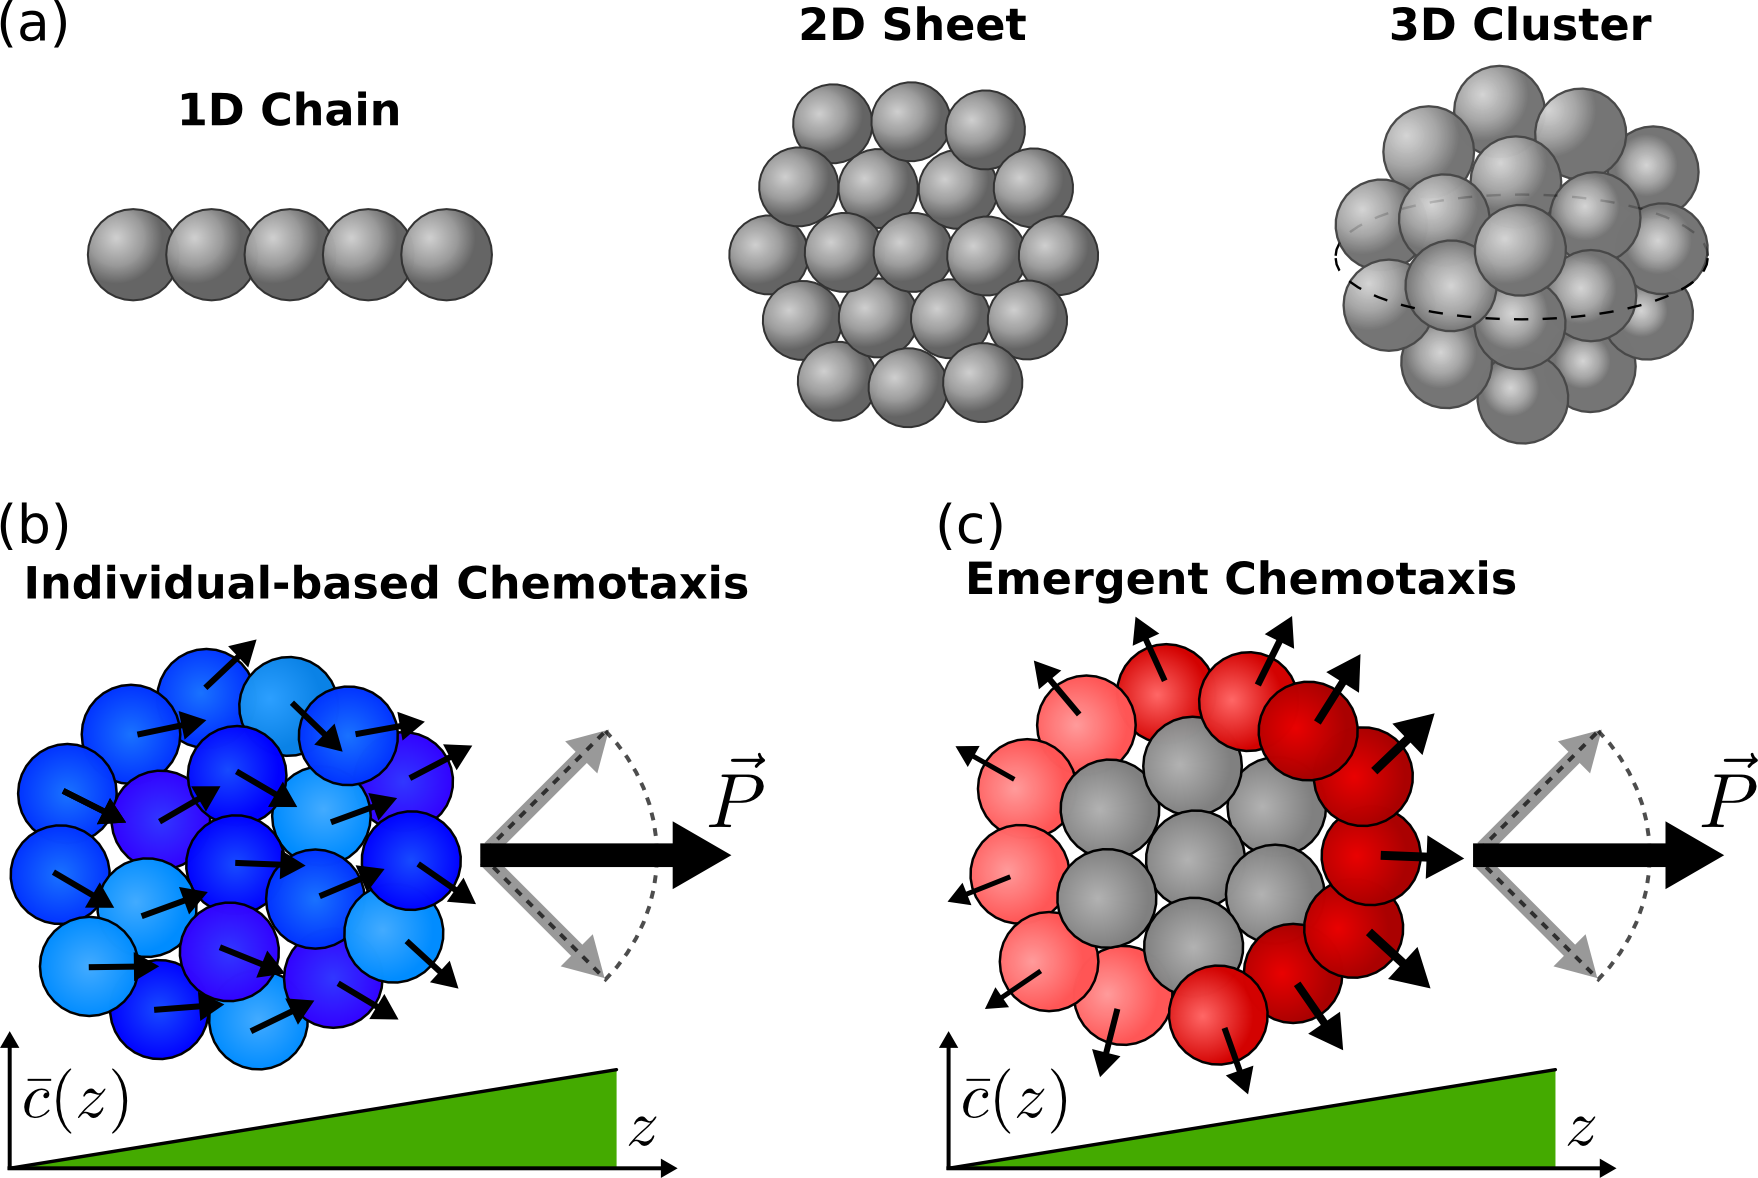
\includegraphics[width=0.8\textwidth]{../fig/ch3_fig1.png}
    \caption{(a) We study the chemotactic performance of 1D chains, 2D sheets, and 3D clusters of cells. (b) In individual-based chemotaxis (IC), cells in the collective polarize based on their own gradient measurement. (c) In emergent chemotaxis (EC), cell polarization depends on intercellular interactions: cells on the edge polarize based on their measurement of the concentration, and cells in the bulk do not polarize. In both mechanisms the total polarization $\vec{P}$ will fluctuate in magnitude and direction due to noise in cell measurements.} \label{fig:ch3_1}
\end{figure}


\section{Individual-based Chemotaxis}

We first consider IC [Fig.\ \ref{fig:ch3_1}(b)]. Due to the chemoattractant molecules in the environment, each cell $i$ becomes polarized with vector $\vec{p}_i$ in its desired direction of motion \cite{jilkine2011comparison}. The components of $\vec{p}_i$ reflect the difference in concentration $c(\vec{r},t)$ between the front and back of the cell in each respective direction.
The concentration difference is encoded internally as a weighted count of the molecules within the cell volume. The weighting function will depend on the sensory network, but will generally be positive at the front and negative at the back; here we choose cosine for simplicity. Orienting our coordinate system such that $\hat{z}$ is parallel to the gradient, the components of $\vec{p}_i$ become
\begin{equation}
    p_{i\alpha}(t) = \int_{U_i} d^3r \ w_\alpha(\hat{r}) c(\vec{r},t) , \label{eq:ICcell}
\end{equation}
with $U_i$ the cell volume, $\alpha\in\{x,y,z\}$, and in spherical coordinates the cosine is $w_\alpha(\hat{r}) = \{\sin\theta \cos\phi, \sin\theta \sin\phi, \cos\theta\}$.

To investigate $\langle P_z\rangle$ and $\epsilon^2$ for the IC model,
we first perform particle-based simulations of the chemoattractant in the presence of the permeable cells \cite{ch3code}. A complete description of the simulations used can be found in Section \ref{sct:ch3_sim}. We find that the total mean polarization $\langle \vec{P} \rangle$ points solely in the gradient direction with equal magnitude regardless of dimensionality [Fig.\ \ref{fig:ch3_2}(a), blue data points]. Indeed, Eq.\ \ref{eq:ICcell} indicates that a single cell will have mean polarization proportional to the concentration difference across the cell,
$\langle \vec{p}_i \rangle = \pi a^4g/3 \ \hat{z}$,
regardless of the cell's location.
Therefore the mean collective polarization is geometry-independent, depending only on the number of cells present,
\begin{equation} \label{eq:ICmean}
    \langle \vec{P} \rangle_\text{IC} = \frac{\pi}{3} a^4gN \ \hat{z},
\end{equation}
as shown in Fig.\ \ref{fig:ch3_2}(a) (blue lines).

\begin{figure}[ht]
    \centering
        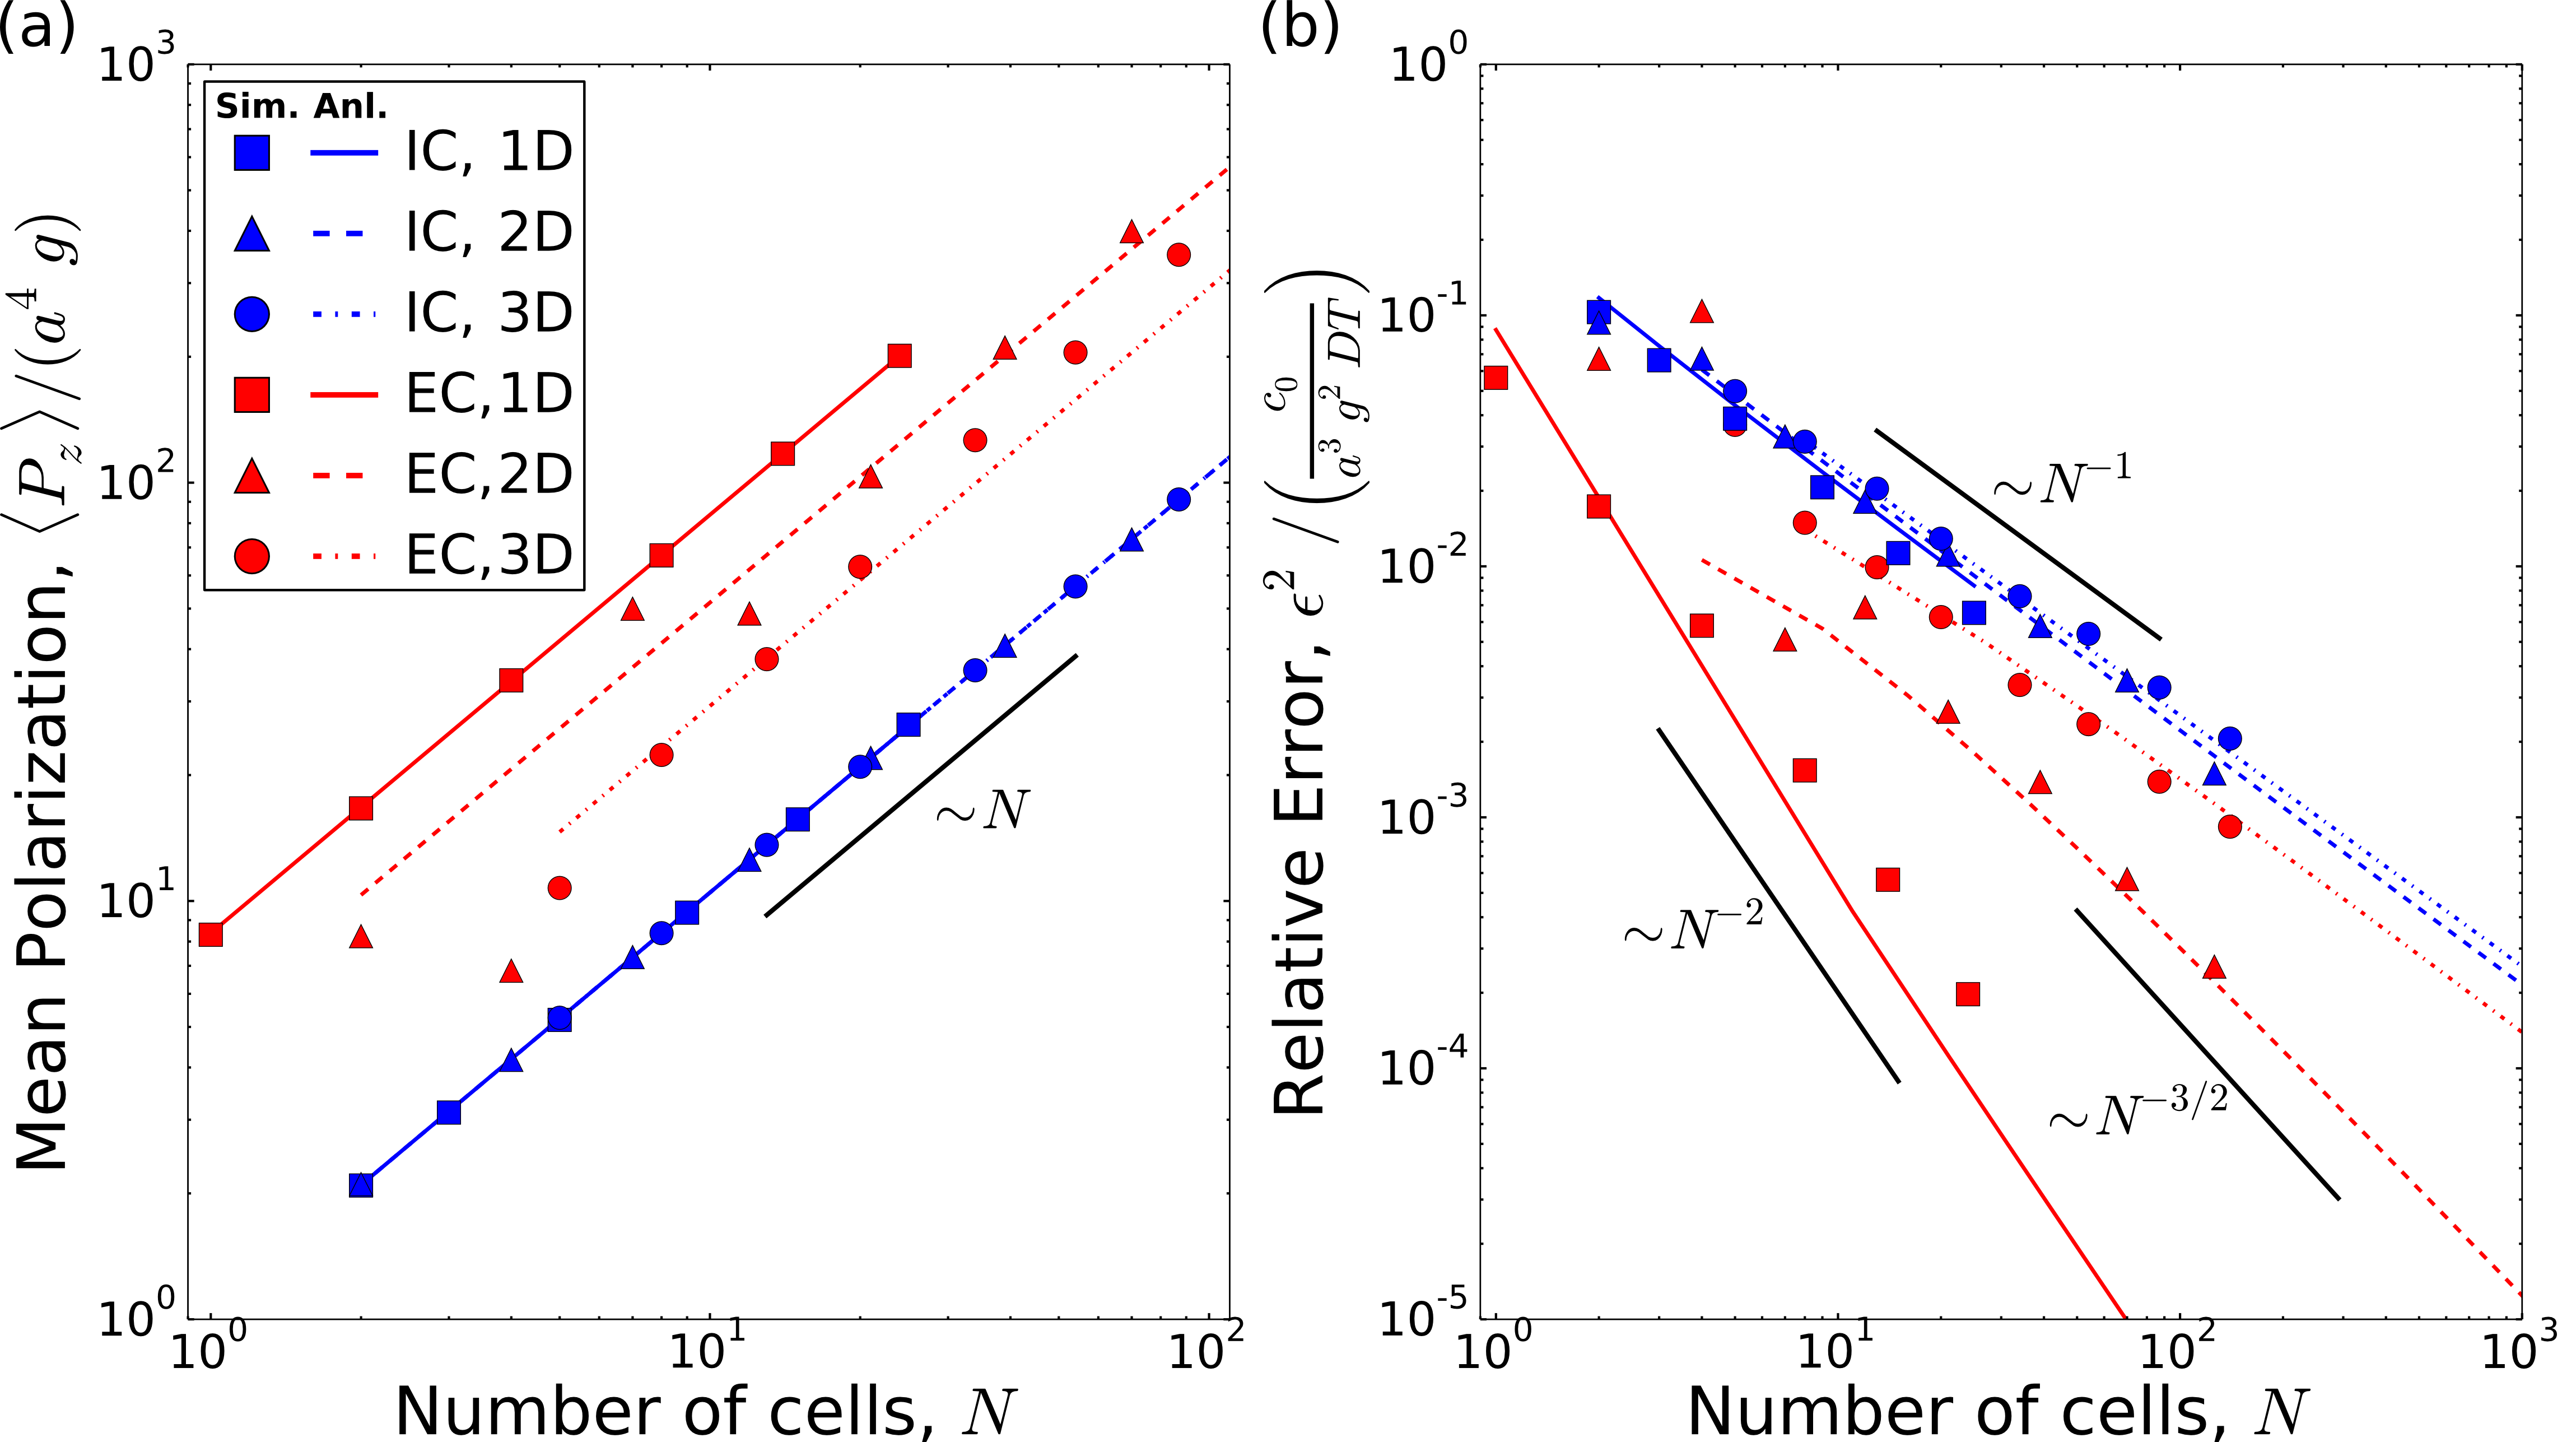
\includegraphics[width=0.8\textwidth]{../fig/ch3_fig2.png}
    \caption{(a) Mean cluster polarization and (b) relative error for both mechanisms of collective chemotaxis in every configuration. Points are simulation data, colored lines are analytical predictions. 1D EC data plotted with respect to $N-1$.} \label{fig:ch3_2}
\end{figure}

We next investigate the relative error for IC collectives. Simulations show that the error decreases with cluster size as
$\epsilon^2 \sim N^{-1}$
for all three geometries [Fig.\ \ref{fig:ch3_2}(b), blue data points]. This is the result that one would obtain if the cells were independent sensors, since both the mean and variance scale with $N$ in that case \cite{simons2004many}. However, they are not independent: their noise is correlated by fluctuations in the concentration \cite{fancher2016fundamental,mugler2016limits}. To understand why correlations do not affect the relative error we investigate the model analytically.

We begin by linearizing the concentration $c(\vec{r},t) = \bar{c}(\vec{r}) + \delta c(\vec{r},t)$ as well as the cell polarization
$\vec{p}_i(t) = \langle \vec{p}_i \rangle + \delta\vec{p}(t)$,
and by Fourier transforming in both space and time we derive analytic expressions for
$\text{Var}[P_z]$ and thereby $\epsilon^2$ (see Sect.\ 3.6). Since
$P_z = \sum_{i=1}^N p_{iz}$,
the variance in the total polarization is a linear combination of all cell polarization variances and covariances present in the collective,
\begin{equation} \label{eq:ICvar1}
    \text{Var}[P_z] =
    \sum_{i} \text{Var}[p_{iz}]
    + \sum_{i\neq j} \text{Cov}[p_{iz},p_{jz}]
    \equiv V + C ,
\end{equation}
The variance and covariance for cells within the collective are derived from the power spectrum in polarization cross correlations, taking the general form
\begin{align} \label{eq:ICvar2}
\begin{split}
    \text{Cov}[p_{i\alpha},p_{j\alpha}] &= \frac{1}{T}
    \lim_{\omega \to 0} \int \frac{d\omega'}{2\pi}
    \langle\delta\tilde{p}_{i\alpha}^*(\omega')\delta\tilde{p}_{j\alpha}(\omega) \rangle
    \ ,
\end{split}
\end{align}
with $T$ the cell's measurement integration time and $\text{Var}[p_{i\alpha}] = \text{Cov}[p_{i\alpha},p_{i\alpha}]$ \cite{fancher2016fundamental,mugler2016limits,bialek2005physical}. Eq.\ \ref{eq:ICvar2} assumes that the integration time is larger than the timescale of molecule diffusion over the radius $R$ of the collective,
$T \gg \tau_D = R^2/D$, though we relax this assumption in later simulations.
Following this procedure we find that $V$ and $C$ for IC are (see Sect.\ 3.6)
\begin{align}
    V_\text{IC} &= \frac{4\pi a^5c_0}{45DT} N  \label{eq:ICV} , \\
    C_\text{IC} &= -\frac{\pi a^5c_0}{18DT} \sum_{i \neq j}^N \frac{3\cos^2\Theta_{ij}-1}{n^3_{ij}} . \label{eq:ICC}
\end{align}
Here
$n_{ij}$
is the number of cell radii separating the centers of cells $i$ and $j$, and $\Theta_{ij}$ is the angle between the gradient direction and a line connecting the two cells. A detailed derivation of these analytic results can be found in Section \ref{sct:ch3_SI}.

$V_\text{IC}$ scales with $N$ since each cell is involved in gradient sensing and in turn polarizes. However, Eq.\ \ref{eq:ICC} reveals an angular dependence on IC cell cross-correlations. A pair of cells can be correlated or anti-correlated depending on their locations relative to the gradient. Consider a pair of adjacent IC cells that are aligned parallel to the gradient ($\cos^2\Theta_{ij}=1$).
If a fluctuation causes an excess in chemoattractant near the boundary of the two cells, then the down-gradient cell will detect a molecule increase in its front half, resulting in an increased polarization; whereas the up-gradient cell will detect a molecule increase in its back half, resulting in a decreased polarization. The end result is an anti-correlation between the two cells. The opposite effect occurs if the two adjacent cells are aligned perpendicular to the gradient: fluctuations will affect both cells in the same way, causing positive correlations. Since contributions to $C_\text{IC}$ are dependent on cell pair locations, $C_\text{IC}$ itself will be dimensionality dependent because the angles made between cells are determined by geometry.

For a 1D chain of IC cells, every pair is parallel to the gradient resulting in anti-correlated measurements which we find in total scale as $N$ (see Sect.\ 3.6). As dimensionality increases, more and more pairs of cells will be perpendicular to the gradient resulting in reduced anti-correlations in the collective. This culminates in 3D clusters having zero cell-cell covariance contribution to the total cluster variance (see Sect.\ 3.6). The result is that $\epsilon^2 \sim N^{-1}$ regardless of dimensionality, indicating that IC cells behave as effectively independent gradient sensors, even though there are diffusion-mediated cross-correlations between cells. The scalings for $V$ and $C$ are summarized in Table \ref{table:1}. The resulting $\epsilon^2$ predictions are plotted in Fig.\ \ref{fig:ch3_2}(b) (blue lines), and we see excellent agreement with the simulations.


\begin{table}[t]
\normalsize
\begin{center}
\begin{tabular}{cc|l|l|l|l|}
\cline{3-6}
& & $\langle P_z \rangle$ & $V$ & $C$ &
$\epsilon^2$ \\ \cline{1-6}
\multicolumn{1}{ |c| }{ }&&&&&\\[-1em]
\multicolumn{1}{ |c  }{\multirow{3}{*}{IC} } &
\multicolumn{1}{ |c| }{ 1D } & $N^{1}$ & $N^{1}$ & $-N^{1}$ & $N^{-1}$ \\
\multicolumn{1}{ |c| }{ }&&&&&\\[-1em]
\cline{2-6}
\multicolumn{1}{ |c| }{ }&&&&&\\[-1em]
\multicolumn{1}{ |c  }{} &
\multicolumn{1}{ |c| }{ 2D } & $N^{1}$ & $N^{1}$ & $-N^{1}$ & $N^{-1}$ \\
\cline{2-6}
\multicolumn{1}{ |c| }{ }&&&&&\\[-1em]
\multicolumn{1}{ |c  }{} &
\multicolumn{1}{ |c| }{ 3D } & $N^{1}$ & $N^{1}$ & $0$ & $N^{-1}$ \\
\hhline{|==|=|=|=|=|}
\multicolumn{1}{ |c| }{ }&&&&&\\[-1em]
\multicolumn{1}{ |c  }{\multirow{3}{*}{EC} } &
\multicolumn{1}{ |c| }{ 1D } & $N^1$ & $N^0$ & $-N^{-1}$ & $N^{-2}$ \\
\cline{2-6}
\multicolumn{1}{ |c| }{ }&&&&&\\[-1em]
\multicolumn{1}{ |c  }{} &
\multicolumn{1}{ |c| }{ 2D } & $N^1$ & $N^{1/2}$ & $N^{1/2}$ & $N^{-3/2}$\\
\cline{2-6}
\multicolumn{1}{ |c| }{ }&&&&&\\[-1em]
\multicolumn{1}{ |c  }{} &
\multicolumn{1}{ |c| }{ 3D } & $N^1$ & $N^{2/3}$ & $N^1$ & $N^{-1}$ \\
\cline{1-6}
\end{tabular}
\caption{Summary of scaling behavior. $N$ dependence of the leading order term for the mean $\langle P_z \rangle$, and the variance ($V$) and covariance ($C$) contributions to the relative error $\epsilon^2 = (V+C)/\langle P_z \rangle^2$. $C$ for EC in 2D has a $\log$ correction (see Sect.\ 3.6).}
\label{table:1}
\end{center}
\end{table}


\section{Emergent Chemotaxis}

Next we turn our attention to EC, the mechanism in which grouped cells sense and migrate differently than individuals.
Often cells in a cluster differentiate, with edge cells polarized and bulk cells unpolarized \cite{malet2015collective,cai2016modeling}. In accordance with previous studies \cite{camley2016emergent,varennes2016collective},
we assume that cell interactions are mediated by contact inhibition of locomotion \cite{mayor2010keeping}. The interactions result in edge cells polarized away from their neighbors, and interior cells that remain uninvolved in chemical sensing and do not polarize [Fig.\ \ref{fig:ch3_1}(c)]. The edge cells polarize with strength proportional to the local concentration which, again like Berg and Purcell's perfect instrument \cite{berg1977physics}, is estimated by counting the molecules present within their cell volume. Hence we define the polarization of the $i$th cell in the collective as
\begin{equation} \label{eq:ECcell1}
    \vec{p}_i(t) =
    \begin{cases}
         \hat{r}_i \int_{U_i} d^3r \ c(\vec{r},t) &i \in \{ N_\text{edge} \} \\
        0 &i \in \{ N_\text{bulk} \} \ ,
    \end{cases}
\end{equation}
where $\hat{r}_i$ points radially outwards from the collective, and $U_i$ is the cell volume. Eq.\ \ref{eq:ECcell1} dictates that $\vec{p}_i$ is dependent on a cell's location relative to the collective. As illustrated in Fig.\ \ref{fig:ch3_1}(c), only the cells on the edge sense the chemoattractant, polarizing with a larger magnitude on the high concentration side of the collective. The total polarization depends only on the cells along the edge:
$\vec{P} = \sum_{i \in \{N_\text{edge}\} } \vec{p}_i$.

Simulations for EC show that the mean polarization $\langle P_z \rangle$ scales with $N$ for all geometries [Fig.\ \ref{fig:ch3_2}(a), red points] even though $N_\text{edge}$ is dependent on the dimensionality of the collective. Our analytical solution helps us understand this result. For 1D EC, only the two opposing cells are polarized so $\langle\vec{P}\rangle$ can be solved for exactly, but for 2D and 3D we take the continuum limit of
$\vec{P} = \sum_i \vec{p}_i$,
assuming the collective is much larger than a single cell $R \gg a$ (see Sect.\ 3.6). The resulting expressions are
\begin{equation} \label{eq:ECmean}
    \langle \vec{P} \rangle_\text{EC} = f_d a^4gN \ \hat{z},
\end{equation}
where the prefactors are $f_d = \{8\pi/3, 2\pi^2/3, 16\pi/9\}$ for $d=\{1,2,3\}$ dimensions, and for $d=1$ we have taken $N-1\to N$ for large $N$. Eq.\ \ref{eq:ECmean} is shown in Fig.\ \ref{fig:ch3_2}(b) (red lines), and we see good agreement. $\langle P_z \rangle$ scales with $N$ because it depends on the product of
$N_\text{edge} \sim N^{(d-1)/d}$
and the distance spanned in the gradient direction by the collective
$R \sim N^{1/d}$,
resulting in a mean polarization which is geometry invariant \cite{malet2015collective}.

Comparing EC and IC shows that $\langle P_z \rangle \sim N$ regardless of collective migration mechanism or geometry as seen in Fig.\ \ref{fig:ch3_2}(a). $\langle P_z \rangle$ has the same parameter dependency for both EC and IC, namely $a^4g$, which is the average change in the number of chemoattractant molecules across a cell. Although
$\langle P_z \rangle_\text{EC} \approx 6 \langle P_z \rangle_\text{IC}$
meaning that EC speed is faster than IC, this relatively small difference may be difficult to detect in biological systems. Moreover, both mechanisms have the same $N$ scaling.
Does the same equivalence between EC and IC also hold for the relative error?

Interestingly, simulations show that the EC relative error does depend on geometry and in fact outperforms IC in terms of scaling in 1D and 2D [Fig.\ \ref{fig:ch3_2}(b), red points]. Only in 3D does the relative error appear to scale the same as IC. In order to understand the dimension dependence of the EC relative error we again investigate the model analytically.
Following the procedure outlined by Eqs.\ \ref{eq:ICvar1} and \ref{eq:ICvar2} we find analytic expressions for $\text{Var}[P_z] = V + C$ for EC,
\begin{align}
    V_\text{EC} &= \frac{16\pi a^5c_0}{15DT} \sum_{i=1}^{N_\text{edge}} \cos^2\Theta_i \label{eq:ECV} , \\
    C_\text{EC} &= \frac{8\pi a^5c_0}{9DT} \sum_{i \neq j}^{N_\text{edge}} \frac{\cos\Theta_i\cos\Theta_j}{n_{ij}} , \label{eq:ECC}
\end{align}
with $\Theta_i$ the angle $\hat{r}_i$ makes with the gradient. Again, a detailed derivation of these results can be found in Section \ref{sct:ch3_SI}. Both $V_\text{EC}$ and $C_\text{EC}$ depend on dimensionality simply because $N_\text{edge} \sim N^{(d-1)/d}$. From Eqs.\ \ref{eq:ECV} and \ref{eq:ECC} we see that
$V \sim N_\text{edge}$,
and that $C$ depends on the angles edge cells make with the gradient. The angular dependence means that cells along the front and back sides of the cluster (relative to the gradient) are strongly anti-correlated since $\cos\Theta_i\cos\Theta_j \approx -1$,
whereas pairs of edge cells near the middle are very weakly correlated ($\cos\Theta_i\cos\Theta_j \approx 0$). Unlike in the case of IC, the scaling of $C$ with $N$ increases with dimensionality as summarized in Table \ref{table:1}, and the resulting $\epsilon^2$ predictions show good agreement with the simulation results [Fig.\ \ref{fig:ch3_2}(b)].

The dimension dependence of the EC relative error can be understood by thinking of the collective as one large detector whose sensory surface is comprised of two halves. If both halves were to take measurements of their local concentrations and then polarize in opposing directions with strengths proportional to their measurements, then $\epsilon^2$ would depend on the radius of each half
$a_\text{eff}$
and their separation distance
$A_\text{eff}$ according to $\epsilon^2  \sim a^{-1}_\text{eff}A^{-2}_\text{eff}$ \cite{mugler2016limits}.
The radius of each half is independent of $N$ for a 1D chain (each half is a single cell), but it scales as
$a_\text{eff} \sim N^{1/d}$ for $d = 2$ or $3$ dimensions.
The separation distance scales with the \r{radius} of the collective for all $d$,
$A_\text{eff} \sim N^{1/d}$. This results in
$\epsilon^2 \sim \{N^{-2}, N^{-3/2}, N^{-1}\}$ for $d=\{1,2,3\}$ [Fig.\ \ref{fig:ch3_2}(b), black lines],
which agree with the scalings seen in simulations and analytics.

Thus, the physical origin of the advantage of EC over IC lies in how the errors scale with the collective size $N$. In IC, all $N$ cells contribute to the sensing, and cross-correlations between them scale either linearly or sublinearly with $N$, leading to a scaling $\epsilon^2 \sim 1/N$ that is characteristic of independent sensors. But in EC, only $N_\text{edge} \sim N^{(d-1)/d}$ cells contribute to the sensing, leading to a sublinear scaling with $N$ of the variance contributions of the individual cells. The total variance of the collective, then, depends on the cross-correlations, which are geometry-specific: in 1D they are dwarfed by the individual variances, in 2D they are commensurate, and in 3D they dominate (Table \ref{table:1}). As a result, 1D and 2D EC collectives benefit from a variance that scales subextensively, i.e., sublinearly with $N$.

\section{Model Extensions}

\begin{figure}[ht]
    \centering
        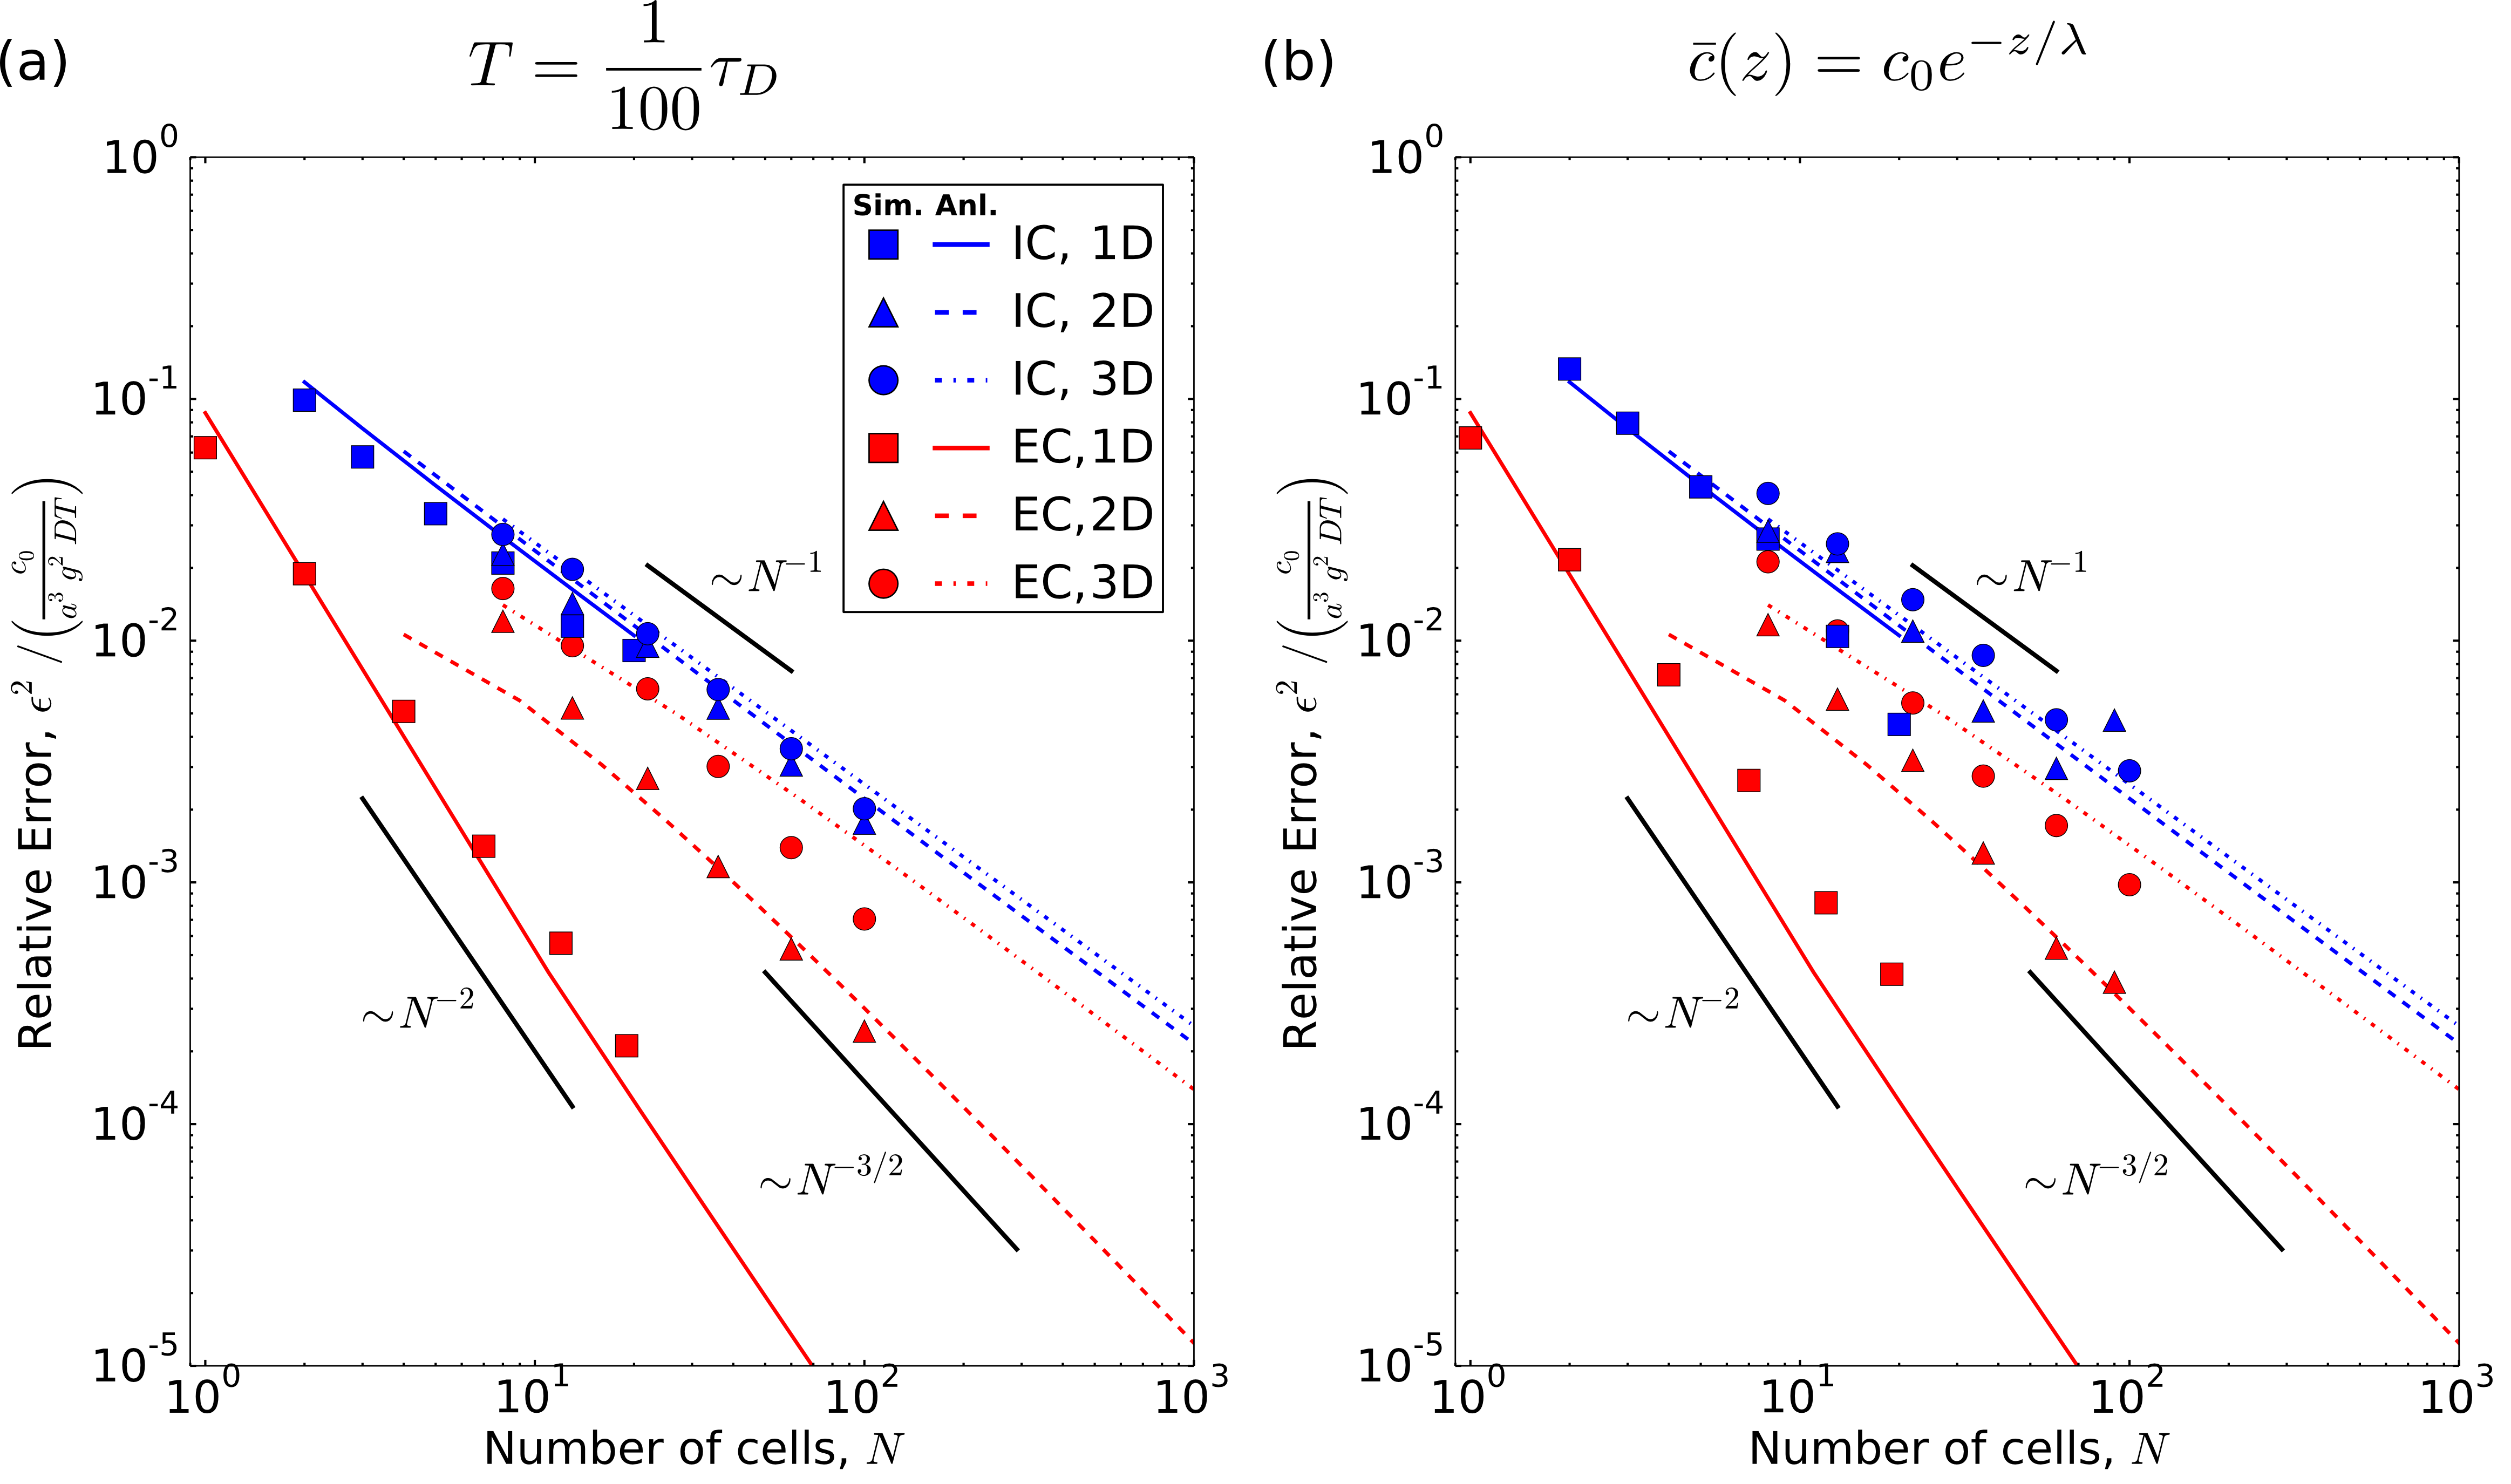
\includegraphics[width=0.8\textwidth]{../fig/ch3_si1.png}
    \caption{(a) Short-time integration relative error results. Data points are of simulations for $T= \frac{1}{100} \tau_D$. (b) Exponential concentration profile relative error results. The mean concentration profile is $\bar{c}(z) = c_0 e^{-z/\lambda}$, the lengthscale $\lambda=\sqrt{D/\beta}$ is set by the diffusion coefficient $D$ and the molecule decay rate $\beta$. Lines are from original analytical predictions using $T > \tau_D$ and a linear concentration profile.} \label{fig:ch3_3}
\end{figure}

Our analytical treatment relies on several assumptions which we now relax using the simulations. In Fig.\ \ref{fig:ch3_2} the integration time $T$ is larger than the timescale for molecule diffusion $\tau_D$.
We relax the assumption that the integration time $T$ must be larger than the timescale for diffusion $\tau_D \sim R^2/D$ [Fig.\ \ref{fig:ch3_3}(a)]. We find that $\epsilon^2$ scales the same way as previously predicted for both EC and IC, even when $T = \tau_D/100$. The only exception is that $\epsilon^2$ for 3D EC [Fig.\ \ref{fig:ch3_3}(a), red circles] has a more negative power-law dependence on $N$ than the expected $\sim N^{-1}$. The shorter integration time results in decreased correlations between edge cells which when $T>\tau_D$ results in $C\sim N$. Hence with
$T < \tau_D$
the total variance is less dependent on $C$, and $V \sim N^{2/3}$ becomes the dominant contribution to $\text{Var}[P_z]$ in the case of 3D EC. This results in a steeper scaling of $\epsilon^2$ closer to
$\text{Var}[P_z]/\langle P_z \rangle^2 \sim N^{2/3}/N^2 = N^{-4/3}$.
Interestingly, we see that relaxing the assumption $T \gg \tau_D$ results in improved precision for EC over IC not just in 1D and 2D but also in 3D configurations.

In Fig.\ \ref{fig:ch3_3}(b) we change the concentration profile from linear to exponential which has a mean concentration of
$\bar{c}(z) = c_0 e^{-z/\lambda}$.
The lengthscale $\lambda=\sqrt{D/\beta}$ depends on the diffusion coefficient and the molecule degradation rate $\beta$. In Fig.\ \ref{fig:ch3_3}(b) the simulation results are for $\lambda > a$. We find that $\epsilon^2$ is in very good agreement with our original analytic predictions. The only exception is that due to the exponential profile, $\langle P_z \rangle$ for 1D EC (Fig.\ \ref{fig:ch3_3}(b), red squares) is non-linear in $N$ causing the relative error data to scale less steeply than the expected $N^{-2}$.

In our model, IC polarization is adaptive to the background concentration as observed in the Ras signalling pathway for \textit{Dictyostelium discoideum} chemotaxis \cite{takeda2012incoherent}. On the other hand, our EC model is non-adaptive. Cell polarization increases with background concentration causing tension in the collective [Fig.\ \ref{fig:ch3_1}(c)], as previously studied \cite{camley2016emergent}. However, adaptive collective sensing has been observed in mammary epithelial cells \cite{ellison2016cell}. Our EC model could be made adaptive by replacing the integrand in Eq.\ \ref{eq:ECcell1} with
$c(\vec{r}+\vec{r}',t)-c_0$.
This change does not affect the properties of $\vec{P}$ since the background concentration cancels out when summing over all edge cells, but it does remove the internal tension in the collective.

\section{Paradigms of EC and IC Behavior}

Both models are paradigmatic, and encompass many observed collective chemotaxis strategies in biology.
Known strategies of collective cell chemotaxis fall broadly into five categories. First, experiments focused on CIL have revealed collective cell streaming in which each cell makes independent protrusions \cite{mayor2010keeping}. Second, experiments discussed in Refs.\
\cite{cai2016modeling,friedl2009collective,haeger2015collective,malet2015collective}
all show behavior wherein edge cells exhibit an active, motile phenotype or make outward protrusions. Third, studies detailed in Refs.\
\cite{theveneau2010collective,friedl2012classifying,cheung2013collective}
illustrate cellular behavior wherein active, motile cells form one or more multicellular chain-like protrusions extending from the collective. Fourth, experiments on epithelial organoids demonstrated that chemical communication between cells can underlie collective gradient sensing \cite{ellison2016cell}. Finally, recent modeling studies have highlighted the role played by cell rearrangement within the collective in governing collective chemotaxis
\cite{camley2016emergent,camley2016collective}.

The first strategy in which cells act independently is directly described by the IC models. The second strategy in which edge cells make outward protrusions is exemplary of the EC model. The third strategy may be considered as a combination of our IC and EC models: the cell at the tip of the multicellular protrusion is often of a highly invasive phenotype akin to our EC edge cells, while the cells within the bulk of the protrusion are less invasive and may behave like bulk cells or IC cells depending on their activity. In the case of the fourth strategy, the error in the communication process will contribute additional noise to the collective polarization \cite{mugler2016limits}, and when communication is optimal we recover the same scaling relationship for the relative error as in our EC model, as discussed at the end of Sect.\ 3.3. Finally, the fifth strategy, namely collective chemotaxis in which cells rearrange, is not encompassed by our IC and EC models, since we consider cell locations to be fixed relative to the collective. It may very well be that cell rearrangement allows for spatial fluctuations, and thereby correlations, to be averaged out resulting in a quantitatively improved relative error. This is an interesting avenue of further research.

\section{Discussion}

Besides the advantage revealed here in terms of chemotactic precision, there may be other natural advantages to EC. In EC only edge cells are involved in chemical sensing and polarization, freeing bulk cells from receptor and protein production necessary for chemotaxis. Bulk cells are free to differentiate into other phenotypes, which is in stark contrast with IC where every cell must be of the polarized phenotype. Additionally, EC provides a simple solution to bulk cells being shielded from the diffusing chemoattractant by edge cells. This phenomenon is especially important for 3D collectives where it can significantly impact the sensory precision of bulk cells \cite{smith2016role}.

The above advantages may be why EC-style collective migration is more prevalent than IC. For example, EC has been observed in two dimensional collectives of malignant lymphocytes \cite{malet2015collective} and in border cell migration \cite{cai2016modeling}. In cancer, metastatic invasion sometimes occurs in the form of chains of cells leaving the tumor with a leader cell at the front \cite{cheung2013collective,friedl2009collective}, analogous to our 1D EC model. Two-dimensional EC migration may also be implicated in tumorigenesis and metastasis in pancreatic ductal cells given the cylindrical surface-like geometry of pancreas ducts
\cite{bardeesy2002pancreatic}. Although we only study idealized collective shapes, the dimensionality-dependent scalings we derive are likely to persist in these systems because the scalings are independent of the exact shapes used.

How can our predictions be tested in experiments? The chemotactic index (CI), commonly defined as
$\text{CI} \equiv \langle \cos\theta \rangle$ where $\theta$ is the angle between the trajectory and the gradient \cite{van2007biased}, is actually a simple monotonic function of $\epsilon^2$. For small deviations from perfect chemotaxis, we have
$\text{CI} \approx 1 - \langle \theta^2 \rangle/2 = 1 - \text{Var}[\theta]/2$.
If $v_z$ and $v_x$ are the components of the velocity of the collective parallel and perpendicular to the gradient, respectively, then $\theta \approx v_x/v_z$ with $\langle v_z\rangle > 0$ and $\langle v_x\rangle = 0$, resulting in
$\text{Var}[\theta] = \text{Var}[v_z] / \langle v_z\rangle^2 = \epsilon^2$.
Therefore the relative error and chemotactic index are related as
$\text{CI} = 1 - \epsilon^2/2$ for small errors.
With this relationship the predicted scalings of $\epsilon^2$ for EC and IC may be tested with chemotaxis experiments. Additionally, the
CI scaling behavior could be used to determine whether an EC- or IC-style migration is at play in a system of collective chemotaxis.

We have shown how the fluctuations in a diffusing attractant concentration set physical limits to collective chemotactic performance. By focusing on two fundamental classes of collective chemotaxis, we have found that the mean polarization scales with the size of the collective irrespective of the mechanism or geometry, but that the emergent mechanism outperforms an individual-based one for 1D and 2D geometries in terms of chemotactic precision.
This advantage arises due to the ways that errors accumulate in the two mechanisms: in an emergent strategy, fewer cells contribute their sensory noise to the collective, and in 1D and 2D the cross-correlations between cells remain low, ultimately leading to a subextensive scaling of polarization variance with collective size. As such, the performance advantage is an inherent property of the emergent mechanism, and we suspect that it not only helps explain the prevalence of emergent chemotaxis in cellular systems, but that it also is detectable using standard measures such as the chemotactic index.


\section{Description of Simulations} \label{sct:ch3_sim}

Computational simulations are performed to test the properties of EC and IC for one, two and three dimensional collectives. In the simulation, the chemical concentration and its dynamics are modeled by a bath of diffusing particles. All particles undergo a 3D random walk within a confined volume, and the volume's boundaries are set to produce the desired chemical concentration profiles. Cells are placed at fixed positions within the 3D volume in either one, two or three dimensional configurations. Particles move freely through cells and do not collide with one another. For a linear concentration profile, one volume boundary produces particles and is reflective, while the boundary on the opposite of the volume absorbs all particles that collide with it. The remaining boundaries are all periodic. For an exponential concentration, the same boundaries are used as in the linear concentration profile, and particles also degrade.

At each time-step of the simulation particles randomly move and are produced. In a given time-step particles move in a random direction with a probability
$p = D\Delta t/b^2$,
with $b$ the particle hopping distance, $D$ the diffusion coefficient, and $\Delta t$ the time-step. A particle is produced during that time-step with probability
$q = k\Delta t$,
with $k$ the production rate. The time-step $\Delta t$ is set such that $p + q \leq 1$. In the case of an exponential concentration profile, particles may also degrade during a time-step. Particles degrade with probability
$r = \beta \Delta t$, with $\beta$ the degradation rate. In this case $\Delta t$ is set such that $p + q + r \leq 1$.

The simulation code used for this paper can be found at \url{https://doi.org/10.5281/zenodo.401040}, and the most up-to-date version of the code can be found at \url{https://github.com/varennes/particletrack}.


\section{Derivation of Analytic Results} \label{sct:ch3_SI}

We consider collectives in one, two and three dimensions of radius $R$ comprised of $N$ cells. Each cell is taken to be a permeable sphere of radius $a$ through which molecules of the surrounding chemical concentration $c(\vec{r},t)$ can freely diffuse. The chemical concentration is taken to be
\begin{equation}
    c(\vec{r},t) = c(0,t) + \vec{r}\cdot\vec{g}(\vec{r},t)
\end{equation}
with $\vec{g}$ parallel to the \textit{z} axis. The chemical concentration obeys normal diffusion
\begin{equation} \label{eq:diffeq}
    \dot{c} = D\nabla^2c+\eta_c
\end{equation}
with $D$ the diffusion coefficient, and $\eta_c$ the Langevin noise due to fluctuations in concentration. We express the concentration as $c(\vec{r},t) = \bar{c}(\vec{r}) + \delta c(\vec{r},t)$ with
\begin{equation} \label{eq:meanc}
    \bar{c}(\vec{r}) = c_0 + \vec{r}\cdot\vec{g}
\end{equation}
where $c_0$ is the mean concentration at the origin. The Langevin noise term $\eta_c$, and the Fourier transformed fluctuation in the concentration $\delta\tilde{c}(\vec{k},\omega)$ have the following properties (see Ref.\ [23] of the main text):
\begin{gather}
    \langle\tilde{\eta}_c(\vec{k}',\omega')\tilde{\eta}_c(\vec{k},\omega) \rangle = 2D \ 2\pi\delta(\omega-\omega') \int d^3y \ \vec{k}\cdot\vec{k}' \ \bar{c}(\vec{y}) \ e^{i\vec{y}\cdot\left(\vec{k}-\vec{k}'\right)} \ ,
    \label{eq:c1} \\
    \langle\delta\tilde{c}(\vec{k}',\omega')\delta\tilde{c}(\vec{k},\omega) \rangle = \frac{\langle\tilde{\eta}_c(\vec{k}',\omega')\tilde{\eta}_c(\vec{k},\omega) \rangle}{(Dk^2-i\omega)(Dk'^2+i\omega')} \ .
    \label{eq:c2}
\end{gather}

Next, we define the cell polarization vectors for individual-based chemotaxis (IC) and emergent chemotaxis (EC). Collectives of $N$ cells form shapes of different dimensionality: a chain of cells of length $2R$ (1D), a disc of cells with radius $R$ (2D), and a sphere of cells of radius $R$ (3D).


\subsection{Individual-based Chemotaxis}

In the IC mechanism, cells independently measure the chemoattractant gradient in order to set their polarization vector $\vec{p}$. For a spherically-shaped cell with volume $U_i$, $\vec{p}_i$ is defined as
\begin{equation}
    p_{i\alpha}(t) = \int_{U_i} d^3r \ w_\alpha c(\vec{r},t) ,
\end{equation}
where $\alpha\in\{x,y,z\}$, and in spherical coordinates the cosine is $w_\alpha = \{\sin\theta \cos\phi, \sin\theta \sin\phi, \cos\theta\}$.
The $x, y, z$ components are written as
\begin{align}
    p_{ix}(t) &= \int d\Omega' \ \sin\theta' \cos\phi' \int_0^a dr' \ r'^2 \ c(\vec{r}_i+\vec{r}',t)  \label{eq:3DMWpx} \\
    p_{iy}(t) &= \int d\Omega' \ \sin\theta' \sin\phi' \int_0^a dr' \ r'^2 \ c(\vec{r}_i+\vec{r}',t)  \label{eq:3DMWpy} \\
    p_{iz}(t) &= \int d\Omega' \ \cos\theta' \int_0^a dr' \ r'^2 \ c(\vec{r}_i+\vec{r}',t), \label{eq:3DMWpz}
\end{align}
where $d\Omega' = \sin\theta'd\theta'd\phi'$. The $r'$ coordinates are relative to the center of the respective cell, and the $r_i$ coordinates are relative to the center of the collective.
Using the mean concentration (Eq.\ \ref{eq:meanc}) with a constant gradient $\vec{g} = g \hat{z}$, we calculate the mean polarization of a single cell:
\begin{align*}
    \langle p_{iz} \rangle &= \int d\Omega' \ \cos\theta' \int_0^a dr' \ r'^2 \ \bar{c}(\vec{r}_i+\vec{r}') \\
    &= \int_0^a dr' \ r'^2 \int d\Omega' \ \cos\theta' (c_0+gr_i\cos\theta_i+gr'\cos\theta') \\
    &= \frac{\pi}{3} a^4 g \ .
\end{align*}
The means for the $x$ and $y$ components are $\langle p_{ix} \rangle = \langle p_{iy} \rangle = 0$ since they are perpendicular to the gradient. On average, cells performing IC migration will only polarize in the $z$ direction. The mean for a collective of IC cells is
\begin{equation}
    \langle \vec{P} \rangle = \frac{\pi}{3} a^4 g N \ \hat{z} \ .
\end{equation}


\subsection{Emergent Chemotaxis}

In EC, cells along the edge of the cluster polarize outwards, whereas cells in the interior are not involved in chemical sensing and remain unpolarized:
\begin{equation}
    \vec{p}_i(t) =
    \begin{cases}
         \hat{r}_i \int_{U_i} d^3r \ c(\vec{r},t) &i \in \{ N_\text{edge} \} \\
        0 &i \in \{ N_\text{bulk} \} \ ,
    \end{cases}
\end{equation}
where $\hat{r}$ points radially outwards from the collective. In order to break down $\vec{p}_i(\vec{r},t)$ into component vectors we must be mindful of the dependence of $\hat{r}_i$ on the cell location. For an edge cell the unit vector $\hat{r}_i$ points in the direction of the cell's location in the collective,
$\hat{r}_i = \sin\Theta_i\cos\Phi_i \hat{x} + \sin\Theta_i\sin\Phi_i \hat{y} + \cos\Theta_i \hat{z}$
where $\Theta_i$ is the polar angle made with the gradient direction and $\Phi_i$ is the azimuthal angle along the collective. The cell component vectors are
\begin{align}
    p_{ix}(t) &= \sin\Theta_i\cos\Phi_i \ p_i(t) , \\
    p_{iy}(t) &= \sin\Theta_i\sin\Phi_i \ p_i(t) \ , \\
    p_{iz}(t) &= \cos\Theta_i \ p_i(t) \ ,
\end{align}
with $p_i(t) = \int_{U_i} d^3r \ c(\vec{r},t)$ and $i \in \{ N_\text{edge}\}$. The total polarization of the collective,
$\vec{P} = \vec{P}_x + \vec{P}_y + \vec{P}_z$,
is a sum of all the component vectors:
\begin{align}
    P_x(t) &= \sum_i^{N_\text{edge}} \sin\Theta_i\cos\Phi_i \ p_i(t) \ , \label{eq:PECx} \\
    P_y(t) &= \sum_i^{N_\text{edge}} \sin\Theta_i\cos\Phi_i \ p_i(t) \ , \label{eq:PECy} \\
    P_z(t) &= \sum_i^{N_\text{edge}} \cos\Theta_i \ p_i(t) \ . \label{eq:PECz}
\end{align}

For an edge cell, the mean polarization is equal to the average number of molecules the cell counts within its spherical body:
\begin{align*}
    \langle \vec{p}_i \rangle &= \int_{U_i} d^3r \ \bar{c}(\vec{r}) \ \hat{r}_i \\
    &= \frac{4\pi}{3}a^3 (c_0+gR\cos\Theta_i) \ \hat{r}_i \ ,
\end{align*}
where $\Theta_i$ is the angle the cell's location makes with the gradient direction. The mean for a cluster of EC cells will depend on the dimensionality of the cluster. For a 1D chain of cells, only the two cells on the opposite ends of the chain are polarized, and $\langle P \rangle$ is the difference in the mean number of molecules counted in between the two edge cells:
\begin{equation} \label{eq:1DECmean}
    \text{1D}: \langle \vec{P} \rangle = \frac{8\pi}{3}a^4g (N-1) \ \hat{z} \ .
\end{equation}

In order to calculate the mean total polarization for two and three dimensional clusters we assume that the cluster size is relatively large ($a\ll R$) and approximate the sum as an integral. For a 2D disc of cells the sum
$\vec{P} = \sum_i^{N_\text{edge}} \vec{p}_i$
becomes an integral over the circumference of the cluster. The circumference and the total number of cells along the edge are related by $2\pi R = 2a N_\text{edge}$, and so a segment along the perimeter of length $R\theta$ is equivalent in length to $2a n$ with $n$ the number of edge cells in that segment. Hence $n =\frac{R}{2a}\theta$ allowing us to write integrals for $\vec{P}(t)$ as
\begin{equation}
    \vec{P}(t) = \frac{R}{2a} \int_0^{2\pi} d\theta \ \vec{p}_i(t) \ .
\end{equation}
The mean polarization will point only in the $z$ direction with magnitude
\begin{equation*}
    \langle P_z \rangle = \frac{R}{2a} \int_0^{2\pi} d\theta \ \langle p_z \rangle = \frac{R}{2a} \int_0^{2\pi} d\theta \ \cos\theta \left( \frac{4\pi}{3}a^3 (c_0+gR\cos\theta) \right) = \frac{2\pi^2}{3} a^2gR^2 \ .
\end{equation*}
Using the relation $N = (R/a)^2$, the mean of the total polarization is
\begin{equation} \label{eq:2DECmean}
    \text{2D}: \langle\vec{P}\rangle = \frac{2\pi^2}{3} a^4gN \ \hat{z} \ .
\end{equation}

Similarly, in 3D we approximate the sum as an integral of the spherical surface of the cluster. A patch on the surface of area $\Omega R^2$ encompasses
$n = \Omega R^2 / (\pi a^2)$ edge cells. The total polarization can therefore be written as an integral over the surface of a spherical cluster:
\begin{equation}
    \vec{P}(t) = \frac{R^2}{\pi a^2} \int d\Omega \ \vec{p}_i(t) \ .
\end{equation}
The mean polarization will point only in the $z$ direction with magnitude
\begin{equation*}
    \langle P_z \rangle = \frac{R^2}{\pi a^2} \int d\Omega \ \langle p_z \rangle = \frac{R^2}{\pi a^2} \int d\Omega \ \cos\theta \left( \frac{4\pi}{3}a^3 (c_0+gR\cos\theta) \right) = \frac{16\pi}{9} agR^3 \ .
\end{equation*}
For a spherical cluster, $N = (R/a)^3$ and the mean of the total cluster polarization is
\begin{equation} \label{eq:3DECmean}
    \text{3D}: \langle\vec{P}\rangle = \frac{16\pi}{9} a^4gN \ \hat{z} \ .
\end{equation}


\subsection{Variance in Cell \& Cluster Polarization}

Here we derive the variance in cell and collective polarizations. The first section gives a general outline for how this is done for either collective migration mechanism. The following sections will derive the specific expressions for IC, and EC and provide scaling arguments for 1D, 2D and 3D geometries.


\subsubsection{General Outline}
Since the total collective polarization is a sum of the cell polarization for IC or EC, the variance in the total polarization takes the general form:
\begin{equation} \label{eq:PVAR1}
\begin{split}
    \text{Var}[P_\alpha] &=
    \underbrace{\sum_{i=1}^N \text{Var}[p_{i,\alpha}]}_\text{variance contribution}
    + \underbrace{\sum_{i\neq j} \text{Cov}[p_{i,\alpha},p_{j,\alpha}]}_\text{covariance contribution} \\
    &\equiv V + C \ ,
\end{split}
\end{equation}
with $\alpha \in \{ x,y,z\}$.
In order to derive an expression for the variance in collective polarization we must first understand the fluctuations occurring in single cell measurements. The fluctuations in the $i^\text{th}$ cell's polarization vector are calculated by linearizing each component,
$p_{i,\alpha}(t) = \bar{p}_{i,\alpha} + \delta p_{i,\alpha}(t)$
and taking the Fourier transform. The Fourier transform of $\delta p_{i,\alpha}(t)$ takes the general form
\begin{equation}
    \delta\tilde{p}_{i,\alpha}(\omega) = \int d^3x_i \int \frac{d^3k}{(2\pi)^3} f(\theta_i,\phi_i) \ \delta\tilde{c}(\vec{k},\omega) \ e^{-i\vec{k}\cdot(\vec{x}_i+\vec{x})}
\end{equation}
where the functional form of $f(\theta_i,\phi_i)$ is dictated by the migration mechanism (EC or IC) and the component $\alpha$.
The cross-spectrum between the $i^\text{th}$ and $j^\text{th}$ cells is
$\langle \delta\tilde{p}_{i,\alpha}^*(\omega') \delta\tilde{p}_{j,\alpha}(\omega) \rangle$. Utilizing the cross-spectrum we can derive an expression for the variance and covariance in the long-time averaged cell polarization by calculating the power spectrum
\begin{equation} \label{eq:sij1}
    S_{ij,\alpha}(\omega=0) = \lim_{\omega \to 0} \int \frac{d\omega'}{2\pi}
    \langle \delta\tilde{p}_{i,\alpha}^*(\omega') \delta\tilde{p}_{j,\alpha}(\omega) \rangle \ .
\end{equation}
The cell polarization variance and covariance is given by:
\begin{align}
    \text{Var}[p_{i,\alpha}] &= \frac{1}{T} S_{ii,\alpha}(0) \ , \\
    \text{Cov}[p_{i,\alpha},p_{j,\alpha}] &= \frac{1}{T} S_{ij,\alpha}(0) \ ,
\end{align}
where $T$ is the averaging time.
With the above expressions for the cell polarization variance and covariance we can solve for Eq.\ \ref{eq:PVAR1} and in turn calculate the relative error for the whole collective. In subsequent sections we show the derivation only for the $z$ component of the polarization since it is parallel to the gradient. The expressions $x$ and $y$ components will be equal to to the $z$ component since the fluctuations in concentration are symmetric in each direction.


\subsection{Individual-based Chemotaxis}
For IC the variance in $P_z$ is
\begin{equation}
    \text{Var}[P_z] = \sum_{i=1}^N \text{Var}[p_{i,z}] + \sum_{i\neq j} \text{Cov}[p_{i,z},p_{j,z}] \equiv V_\text{IC} + C_\text{IC} \ .
\end{equation}
The Fourier-transformed fluctuations in IC cell polarization is
\begin{equation}
    \delta\tilde{p}_{j,z}(\vec{k},\omega) = \int_V d^3x \int \frac{d^3k}{(2\pi)^3} \cos\theta
    \delta\tilde{c}(\vec{k},\omega)
    e^{-i\vec{k}\cdot(\vec{x_i}+\vec{x})} \ .
\end{equation}
The cross-spectrum for the $z$-component between two cells is
\begin{equation} \label{eq:pij1}
\begin{split}
    \langle\delta\tilde{p}_{i,z}^*(\omega')\delta\tilde{p}_{j,z}(\omega) \rangle = \int_V d^3x d^3x' \int \frac{d^3kd^3k'}{(2\pi)^6}
    \cos\theta \cos\theta'
    \langle \delta\tilde{c}^*(\vec{k}',\omega')\delta\tilde{c}(\vec{k},\omega) \rangle
    e^{-i\vec{k}\cdot(\vec{x}_j+\vec{x})} e^{i\vec{k}'\cdot(\vec{x}_i+\vec{x}')} \ .
\end{split}
\end{equation}
We can rewrite Eq.\ \ref{eq:pij1} by noting that only the relative locations of cell $i$ and $j$ are relevant for the cross-spectrum. Let $\vec{r}_{ij} = \vec{x}_i - \vec{x}_j$ and $r_{ij} = |\vec{r}_{ij}|$.
\begin{equation} \label{eq:sij2}
\begin{split}
    \langle \delta\tilde{p}_{i,z}^*(\omega')\delta\tilde{p}_{j,z}(\omega) \rangle = \int_V d^3x d^3x' \int \frac{d^3kd^3k'}{(2\pi)^6}
    \cos\theta \cos\theta' \\
    \langle \delta\tilde{c}^*(\vec{k}',\omega') \delta\tilde{c}(\vec{k},\omega) \rangle
    e^{-i\vec{k}\cdot\vec{x}} e^{i\vec{k}'\cdot(\vec{r}_{ij}+\vec{x}')}
\end{split}
\end{equation}
Plugging in Eq.\ \ref{eq:c2} for
$\langle \delta\tilde{c}^*(\vec{k}',\omega') \delta\tilde{c}(\vec{k},\omega) \rangle$
and writing $\cos\theta$ in terms of spherical harmonic $Y_1^0(\hat{x})$ yields
\begin{align*}
    \langle\delta\tilde{p}_{i,z}^*(\omega')\delta\tilde{p}_{j,z}(\omega) \rangle &= \int_V d^3x d^3x' \int \frac{d^3kd^3k'}{(2\pi)^6}
    \frac{4\pi}{3} Y_1^0(\hat{x})Y_1^0(\hat{x}') \ 2D \\ &\frac{2\pi\delta(\omega-\omega')}{(Dk^2-i\omega)(Dk'^2+i\omega')} \int d^3y \vec{k}\cdot\vec{k}' \bar{c}(\vec{y}) e^{i\vec{y}\cdot(\vec{k}-\vec{k}')}
    e^{-i\vec{k}\cdot\vec{x}} e^{i\vec{k}'\cdot(\vec{r}_{ij}+\vec{x}')} \\
    &= \frac{4D}{3(2\pi)^5} 2\pi\delta(\omega-\omega') \int_V d^3x d^3x' \int d^3kd^3k'd^3y \ Y_1^0(\hat{x})Y_1^0(\hat{x}') \\
    &\frac{\bar{c}(\vec{y}) \ \vec{k}\cdot\vec{k}'\ e^{i\vec{y}\cdot(\vec{k}-\vec{k}')}}{(Dk^2-i\omega)(Dk'^2+i\omega')} e^{-i\vec{k}\cdot\vec{x}} e^{i\vec{k}'\cdot(\vec{r}_{ij}+\vec{x}')}
\end{align*}
Plugging in the above expression for
$\langle\delta\tilde{p}_{i,z}^*(\omega')\delta\tilde{p}_{j,z}(\omega) \rangle$
into $S_{ij,z}(0)$ (Eq.\ \ref{eq:sij1}) and using the specified mean concentration from Eq.\ \ref{eq:meanc}:
\begin{equation}
\begin{split}
    S_{ij,z}(0) = \frac{4}{3(2\pi)^5D} \int_V d^3x d^3x' \int d^3kd^3k'd^3y \ Y_1^0(\hat{x})Y_1^0(\hat{x}') \frac{\vec{k}\cdot\vec{k}'}{k^2k'^2} \\
    (c_0+\vec{g}\cdot\vec{y}) \ e^{i\vec{y}(\vec{k}-\vec{k}')} \ e^{-i\vec{k}\cdot\vec{x}} e^{i\vec{k}'\cdot(\vec{r}_{ij}+\vec{x}')} \ .
\end{split}
\end{equation}
We can break up the expression for $S_{ij,z}(0)$ into two terms: one dependent on the background concentration, the other on the gradient.
\begin{equation} \label{eq:sij3}
\begin{split}
    S_{ij,z}(0) = \frac{4}{3(2\pi)^5D} \int_V d^3x d^3x' \int d^3kd^3k' \ Y_1^0(\hat{x})Y_1^0(\hat{x}') \frac{\vec{k}\cdot\vec{k}'}{k^2k'^2} \ e^{-i\vec{k}\cdot\vec{x}} \\
    e^{i\vec{k}'\cdot(\vec{r}_{ij}+\vec{x}')}
    \left((2\pi)^3 \delta^3(\vec{k}-\vec{k}') c_0 + \int d^3y \ \vec{g}\cdot\vec{y} \ e^{i\vec{y}(\vec{k}-\vec{k}')} \right)
\end{split}
\end{equation}
Let $S_{ij}^1$ represent the background concentration term and $S_{ij}^2$ represent the gradient dependent term in the power spectrum such that $S_{ij,z}(0) = S_{ij}^1 + S_{ij}^2$.
\begin{equation} \label{eq:Sij1MW}
    S_{ij}^1 = \frac{4c_0}{3(2\pi)^2D} \int_V d^3x d^3x' \int d^3k \ Y_1^0(\hat{x})Y_1^0(\hat{x}') \frac{1}{k^2} \ e^{-i\vec{k}\cdot\vec{x}} \
    e^{i\vec{k}\cdot(\vec{r}_{ij}+\vec{x}')}
\end{equation}
\begin{equation} \label{eq:Sij2MW}
\begin{split}
    S_{ij}^2 = \frac{4c_0}{3(2\pi)^5D} \int_V d^3x d^3x' \int d^3kd^3k'd^3y \ Y_1^0(\hat{x})Y_1^0(\hat{x}') \frac{\vec{k}\cdot\vec{k}'}{k^2k'^2} \ \vec{g}\cdot\vec{y} \\
    e^{i\vec{y}(\vec{k}-\vec{k}')} \
    e^{-i\vec{k}\cdot\vec{x}} \
    e^{i\vec{k}'\cdot(\vec{r}_{ij}+\vec{x}')}
\end{split}
\end{equation}
The following expansions will prove useful:
\begin{align}
    e^{-i\vec{k}\cdot\vec{r}} &= 4\pi \sum_{l,m} (-i)^l j_l(kr) Y_l^{m}(\hat{k}) Y_l^{m*}(\hat{r}) \ , \label{eq:planewave} \\
    \vec{a}\cdot\vec{b} &= \frac{4\pi}{3} ab \sum_{m=-1}^1 Y_1^m(\hat{a}) Y_1^{m*}(\hat{b}) \ . \label{eq:dotprod}
\end{align}
Starting with Eq.\ \ref{eq:Sij1MW} we expand all the exponential terms, and we use these expansions in order to evaluate the angular integrals in $S_{ij}^1$.
\begin{equation}
\begin{split}
    S_{ij}^1 = \frac{2^5(2\pi)c_0}{3D} \int_V d^3x d^3x' \int d^3k \ Y_1^{0*}(\hat{x})Y_1^{0*}(\hat{x}') \ \frac{1}{k^2} \\
    \left(\sum_{l_1,m_1}i^{-l_1} j_{l_1}(xk) Y_{l_1}^{m_1}(\hat{x}) Y_{l_1}^{m_1*}(\hat{k}) \right)
    \left(\sum_{l_2,m_2}i^{l_2} j_{l_2}(r_{ij}k) Y_{l_2}^{m_2}(\hat{k}) Y_{l_2}^{m_2*}(\hat{r}_{ij}) \right) \\
    \left(\sum_{l_3,m_3}i^{l_3} j_{l_3}(x'k) Y_{l_3}^{m_3}(\hat{k}) Y_{l_3}^{m_3*}(\hat{x}') \right)
\end{split}
\end{equation}
The angular integrals over $\hat{x}$ and $\hat{x}'$ eliminate the summations over $l_1,m_1$ and $l_3,m_3$.
\begin{equation} \label{eq:Sij3MW}
\begin{split}
    S_{ij}^1 = \frac{2^5(2\pi)c_0}{3D} \int_0^a dx dx' \int d^3k \ \frac{1}{k^2} x^2 x'^2 \ j_{1}(xk) j_{1}(x'k) \ Y_{1}^{0*}(\hat{k}) Y_{1}^{0}(\hat{k}) \\
    \left(\sum_{l_2,m_2}i^{l_2} j_{l_2}(r_{ij}k') Y_{l_2}^{m_2}(\hat{k}') Y_{l_2}^{m_2*}(\hat{r}_{ij}) \right)
\end{split}
\end{equation}
The product of the two spherical harmonics is
\begin{equation*}
    Y_{1}^{0*}(\hat{k}) Y_{1}^{0*}(\hat{k}) = \frac{1}{\sqrt{4\pi}} \left( Y_0^0(\hat{k}) + \frac{2\sqrt{5}}{5} Y_2^0(\hat{k}) \right) \ .
\end{equation*}
Therefore when evaluating the $\hat{k}$ integral in Eq.\ \ref{eq:Sij3MW} only the $l_2=0,m_2=0$ and $l_2=2,m_2=0$ terms of the summation will be non-zero.
\begin{equation}
\begin{split}
    S_{ij}^1 = \frac{2^5(2\pi)c_0}{3D\sqrt{4\pi}} \int_0^a dx dx' \int_0^\infty dk \ x^2 x'^2 \ j_{1}(xk) j_{1}(x'k) \\ \left(j_0(r_{ij}k) Y_0^0(\hat{r}_{ij}) - \frac{2\sqrt{5}}{5} j_2(r_{ij}k) Y_2^0(\hat{r}_{ij}) \right)
\end{split}
\end{equation}
The integrals over $x$ and $x'$ evaluate to:
\begin{equation*}
    \int_0^a dx \ x^2 j_1(kx) = \frac{1}{k^3}\left(2-2\cos(ak)-ak\sin(ak) \right) \equiv \frac{1}{k^3} h(ak) \ .
\end{equation*}
Note that
$Y_0^0(\Theta_{ij},\Phi_{ij}) = \frac{1}{\sqrt{4\pi}}$
, and
$Y_2^0(\Theta_{ij},\Phi_{ij}) = \frac{1}{2} \sqrt{\frac{5}{4\pi}} (3\cos^2\Theta_{ij}-1)$.
The angle $\Theta_{ij}$ is the angle $\hat{r}_{ij}$ makes relative to the gradient direction $\hat{g}$, $\cos\Theta_{ij} = \hat{r}_{ij}\cdot\hat{g}$. The expression for $S_{ij}^1$ reduces to
\begin{equation}
    S_{ij}^1 = \frac{2^4c_0}{3D} \int_0^\infty dk \ \frac{h^2(ak)}{k^6} \ \left[j_0(r_{ij}k) - j_2(r_{ij}k) (3\cos^2\Theta_{ij}-1) \right]
\end{equation}
We can make the integral dimensionless by making the variable substitutions $u \equiv ak$ and $n_{ij} \equiv r_{ij}/a$.
\begin{equation}
    S_{ij}^1 = \frac{2^4c_0a^5}{3D} \int_0^\infty du \ \frac{h^2(u)}{u^6} \left[j_0\left(n_{ij}u\right) - j_2\left(n_{ij}u\right) (3\cos^2\Theta_{ij}-1) \right] \label{eq:s1u1}
\end{equation}
We can break up Eq.\ \ref{eq:s1u1} into two integrals and evaluate them individually. Note that the exact solution to either integral depends parametrically on $n_{ij}$ and that $n_{ij}$ is the number of cells radii separating two cells. If we are evaluating the cross-correlations in one cell then $i=j$ and $n_{ii}=0$; on the other hand, if $i\neq j$ then $n_{ij} \geq 2$ in order to eliminate the possibility of overlapping cells. In either case the expression simplifies to:
\begin{equation}
    S_{ij}^1 =
    \begin{cases}
        \frac{4\pi c_0a^5}{45D} &\ i=j \\
        -\frac{\pi c_0a^5}{18D} \frac{1}{n_{ij}^3}(3\cos^2\Theta_{ij}-1) &\ i \neq j, \ n_{ij} \geq 2
    \end{cases} \ .
\end{equation}
Doing the same set of expansions for $S_{ij}^2$ in Eq.\ \ref{eq:Sij2MW}, and performing the same kind of analysis reveals that the gradient depedendent term is asymmetric under exchange of $i$ and $j$. Therefore when calculating the cluster polarization variance all the $S_{ij}^2$ terms will cancel. The variance contributions $V$ and $C$ are
\begin{align}
    V_\text{IC} &= \sum_{i=1}^N \frac{1}{T} S_{ii,z}(0) = \frac{4\pi a^5c_0}{45DT} N \ , \label{eq:ICV1} \\
    C_\text{IC} &= \sum_{i\neq j}^N \frac{1}{T} S_{ij,z}(0) = -\frac{\pi a^5c_0}{18DT} \sum_{i\neq j}^N \frac{(3\cos^2\Theta_{ij}-1)}{n_{ij}^3} \ \label{eq:ICC1},
\end{align}
resulting in the IC collective total variance
\begin{equation} \label{eq:VIC}
    \text{Var}[P_z] = \frac{\pi a^5c_0}{9DT} \left[ \frac{4}{5}N - \frac{1}{2}\sum_{i\neq j}^N \frac{(3\cos^2\Theta_{ij}-1)}{n_{ij}^3} \right] \ ,
\end{equation}
as in Eqs.\ 6 and 7 in the main text.
Next we will show how Eq.\ \ref{eq:VIC} scales for collectives in one, two and three dimensional configurations.


\subsubsection{One Dimensional Chain}

For a one-dimensional chain of IC cells each cell is aligned parallel to the gradient and the angular dependence of $C_\text{IC}$ (Eq.\ \ref{eq:ICC1}) vanishes,
\begin{equation}
    C_\text{IC} = -\frac{\pi a^5c_0}{18DT} \sum_{i\neq j}^N \frac{2}{n_{ij}^3} \ .
\end{equation}
We evaluate the sum:
\begin{equation*}
    \sum_{i\neq j}^N \frac{1}{n_{ij}^3} = 2 \sum_{i<j}^N \frac{1}{n_{ij}^3} = 2 \sum_{i=1}^{N-1} \frac{N-i}{(2i)^3} = \frac{1}{4}(N H_{N-1}^{(3)} - H_{N-1}^{(2)}) \ ,
\end{equation*}
with $H_n^{(m)} = \sum_{k=1}^n \frac{1}{k^m}$ the generalized harmonic number. This results in a total variance of the form
\begin{equation}
    \text{Var}[P_z] = \frac{\pi a^5c_c}{9DT} \left[ \frac{4}{5}N - \frac{1}{8} \left( N H_{N-1}^{(3)} - H_{N-1}^{(2)} \right) \right] \ .
\end{equation}
For large $N$, $H_{N-1}^{(i)}$ approaches a constant for $i \geq 2$. Therefore, we see that $\text{Var}[P_z]$ scales with $N$ for 1D IC collectives as in Table I of the main text.


\subsubsection{Two Dimensional Sheet}

For a two-dimensional sheet of IC cells, pairs of cells can now make a variety of angles with the gradient, and the angular dependence of $C_\text{IC}$ cannot be easily simplified. In order to find the $N$ scaling for $C_\text{IC}$ we calculate the sum numerically. Since the covariances rapidly fall-off as $1/n^3_{ij}$, we only track nearest neighbor pairs that are less than 3 cell radii apart. The resulting numerical solution to the sum in $C_\text{IC}$ is
\begin{equation*}
    \sum_{i\neq j}^N \frac{3\cos^2\Theta_{ij}-1}{n_{ij}^3}
    = 2 \sum_{i<j}^N \frac{3\cos^2\Theta_{ij}-1}{n_{ij}^3}
    = \frac{1}{4} (1.70 N - 2.67 \sqrt{N} + 0.89) \ .
\end{equation*}
Therefore the expression for $C_\text{IC}$ (Eq.\ \ref{eq:ICC1}) simplifies to
\begin{equation}
    C_\text{IC} = -\frac{\pi a^5c_0}{18DT} (0.43 N - 0.67 \sqrt{N} + 0.22) \ .
\end{equation}
The covariance contribution, $C_\text{IC}$, to leading order scales linearly with $N$.
The total variance becomes
\begin{equation}
    \text{Var}[P_z] = \frac{\pi a^5c_c}{9DT} \left( 0.59 N + 0.33 \sqrt{N} - 0.11 \right) \ .
\end{equation}
We see that for large $N$, $\text{Var}[P_z]$ scales with $N$ for 2D IC collectives as in Table I in the main text.


\subsubsection{Three Dimensional Cluster}

To obtain a scaling for $C_\text{IC}$ in a three dimensional cluster we assume that cluster is large, such that $a \ll R$ and $N \gg 1$. For a given cell we can calculate its contribution to $C_\text{IC}$ by considering the covariance contribution it makes with a set of cells a fixed distance away from it. The equidistant cells form a spherical shell with the principal cell in the center. Adapting Eq.\ \ref{eq:ICC1} for a cell and its spherical shell of covariance pairs yields:
\begin{equation}
    C_\text{cell} = -\frac{\pi a^5c_0}{18DT} \frac{1}{n_\text{shell}^3} \sum_{i_\text{shell}} 3\cos^2\Theta_{i}-1 \ ,
\end{equation}
with $n_\text{shell}$ the radius of the shell in terms of cell radii.
Going to continuum we can calculate the contribution from the cell and all its pairs
\begin{equation}
\begin{split}
    C_\text{cell} = -\frac{\pi a^5c_0}{18DT n_\text{shell}^3} \int_0^{2\pi} d\phi \int_0^{\pi} d\theta \ \sin\theta (3\cos^2\theta-1) \\
    = -\frac{\pi^2 a^5c_0}{9DT n_\text{shell}^3} \int_0^\pi d\theta \ (3\cos^2\sin\theta - \sin\theta) = 0 \ .
\end{split}
\end{equation}
In the last step, we see that the integral vanishes. Thus, the contribution from a single cell and its shell of pairs sum to zero. Repeating this argument for all cells in the cluster results in the total $C_\text{IC} = 0$. Therefore for 3D clusters there is no covariance contribution to the total variance, and $\text{Var}[P_z] = V_\text{IC} \sim N$ as in Table I of the main text.


\subsection{Emergent Chemotaxis Clusters}
For EC the variance in $P_z$ is
\begin{equation}
    \text{Var}[P_z] = \sum_{i=1}^N \text{Var}[p_{i,z}] + \sum_{i\neq j} \text{Cov}[p_{i,z},p_{j,z}] \equiv V_\text{EC} + C_\text{EC} \ .
\end{equation}
The Fourier-transformed fluctuations in IC cell polarization is
\begin{equation}
    \delta\tilde{p}_{i,z}(\vec{k},\omega) = \cos\Theta_i \int_V d^3x \int \frac{d^3k}{(2\pi)^3}
    \delta\tilde{c}(\vec{k},\omega)
    e^{-i\vec{k}\cdot(\vec{x_i}+\vec{x})} \ ,
\end{equation}
with $\Theta_i$ the angle cell $i$ makes with the gradient.
The cross-spectrum for the $z$-component between two cells is
\begin{equation} \label{eq:pijEC1}
\begin{split}
    \langle\delta\tilde{p}_i^*(\vec{k}',\omega')\delta\tilde{p}_j(\vec{k},\omega) \rangle = \cos\Theta_i \cos\Theta_j \int_V d^3x d^3x' \int \frac{d^3kd^3k'}{(2\pi)^6} \\
    \langle \delta\tilde{c}^*(\vec{k}',\omega')\delta\tilde{c}(\vec{k},\omega) \rangle
    e^{-i\vec{k}\cdot(\vec{x}_j+\vec{x})} e^{i\vec{k}\cdot(\vec{x}_i+\vec{x}')} \ .
\end{split}
\end{equation}
Following the same procedure as in the case of IC, we get an expression for $S_{ij}^1$ for EC:
\begin{equation} \label{eq:SijEC1}
    S_{ij}^1 =
    \begin{cases}
        \frac{16\pi c_0a^5}{15D} \cos^2\Theta_i &\ i=j \\
        \frac{8\pi c_0a^5}{9D} \frac{1}{n_{ij}} \cos\Theta_i \cos\Theta_j &\ i \neq j, \ n_{ij} \geq 2
    \end{cases} \ .
\end{equation}
Since again $S^2_{ij}=0$ by symmetry, the variance for any configuration of EC cells is
\begin{align}
    V_\text{EC} &= \frac{16\pi a^5c_0}{15DT} \sum_{i=1}^{N_\text{edge}} \cos^2\Theta_i \ , \label{eq:ECV1} \\
    C_\text{EC} &= \frac{8\pi a^5c_0}{9DT} \sum_{i\neq j} \frac{\cos\Theta_i \cos\Theta_j}{n_{ij}} \ , \label{eq:ECC1}
\end{align}
as in Eqs.\ 10 and 11 in the main text. The resulting total variance is
\begin{equation} \label{eq:ECvarP}
    \text{Var}[P_z] = \frac{8\pi a^5c_0}{3DT} \left[ \frac{2}{5} \sum_{i=1}^{N_\text{edge}} \cos^2\Theta_i +  \frac{1}{3} \sum_{i\neq j} \frac{\cos\Theta_i \cos\Theta_j}{n_{ij}} \right] \ .
\end{equation}


\subsubsection{One Dimensional Chain}

For a one-dimensional chain of cells only the two cells on the opposing ends are polarized. The cell variance contribution to the total variance therefore does not change with increasing cluster size,
\begin{equation}
    V_\text{EC} = \frac{16\pi a^5c_0}{15DT} \sum_{i=1}^{N_\text{edge}} \cos^2\Theta_i = \frac{32\pi a^5c_0}{15DT} \ .
\end{equation}
Therefore $V_\text{EC} \sim N^0$ for 1D collectives. For $C_\text{EC}$ the distance between the two edge cells increases by two cell radii for each cell added to the chain:
\begin{equation}
    C_\text{EC} = \frac{8\pi a^5c_0}{9DT} \sum_{i\neq j} \frac{\cos\Theta_i \cos\Theta_j}{n_{ij}} = -\frac{8\pi a^5c_0}{9DT} \frac{1}{2(N-1)} \ .
\end{equation}
So $C_\text{EC} \sim N^{-1}$ for 1D collectives. To leading order in $N$ the total collective variance depends only on $V_\text{EC}$:
\begin{equation}
    \text{Var}[P_z] = \frac{32\pi a^5c_0}{15DT} \ ,
\end{equation}
and so $\text{Var}[P_z]$ does not depend on collective size for 1D EC as in Table I of the main text.

\subsubsection{Two Dimensional Sheet}

In order to evaluate the variance for a two-dimensional disc of cells we will approximate the sums as integrals over the circumference of the disc as we did in evaluating the mean polarization. Assuming that $a \ll R$ Eq.\ \ref{eq:ECV1} can be written as an integral
\begin{equation}
    V_\text{EC} = \frac{16\pi a^5c_0}{15DT} \frac{R}{2a} \int_0^{2\pi} d\theta \ \cos^2\theta \ .
\end{equation}
Using the relation $N=(R/a)^2$ yields
\begin{equation}
    V_\text{EC} = \frac{8\pi^2 a^5c_0}{15DT} \sqrt{N} \ .
\end{equation}
Hence for 2D EC, the variance contribution $V_\text{EC}$ scales as $\sqrt{N}$.
In order to determine how $C_\text{EC}$ scales with $N$ we approximate the sums over $i$ and $j$ as a double integral, again assuming that $a \ll R$.
\begin{equation}
    C_\text{EC} = \frac{16\pi a^5c_0}{9DT}
    \left( \frac{R}{2a^2} \right) \int_{\Delta/2}^{2\pi-\Delta/2} d\theta_1 \int_{\theta_1+\Delta/2}^{2\pi} d\theta_2 \ \frac{\cos\theta_1 \cos\theta_2}{n(\theta_1,\theta_2)}
\end{equation}
Here $\Delta = 2a/R$ is the anguler separation between two edge cells, and
\begin{equation*}
    n(\theta_1,\theta_2) = \frac{2R}{a} \sin \left( \frac{1}{2}(\theta_2-\theta_1) \right)
\end{equation*}
is the number of cell radii separating two edge cells. Using this expression for $n(\theta_1,\theta_2)$ we evaluate the integral over $\theta_2$:
\begin{equation}
    \begin{split}
        \left( \frac{R}{2a^2} \right) \int_{\Delta/2}^{2\pi-\Delta/2} d\theta_1 \int_{\theta_1+\Delta/2}^{2\pi} d\theta_2 \ \frac{\cos\theta_1 \cos\theta_2}{n(\theta_1,\theta_2)} \\
        = \frac{R}{8a} \int_{\Delta/2}^{2\pi-\Delta/2} d\theta_1 \cos\theta_1 [ -4\left( \cos(\theta_1/2) + \cos(\theta_1+\Delta/2) \right) \\
        -2 \cos\theta_1 \log\left( \tan(\Delta/4) \tan(\theta_1/4) \right) ]
    \end{split}
\end{equation}
Breaking up the integral into four separate terms we find:
\begin{align*}
    &\int_{\Delta/2}^{2\pi-\Delta/2} d\theta_1 \cos\theta_1 \cos(\theta_1/2) = 0 \ , \\
    &\int_{\Delta/2}^{2\pi-\Delta/2} d\theta_1 \cos\theta_1 \cos(\theta_1+\Delta/2) = -\frac{1}{2}\cos(\Delta/2) (\Delta+\sin\Delta-2\pi) \ , \\
    &\int_{\Delta/2}^{2\pi-\Delta/2} d\theta_1 \cos\theta_1 \log\left( \tan(\Delta/4)\right) = -\frac{1}{2} (\Delta+\sin\Delta-2\pi) \tan(\Delta/4) \ , \\
    &\int_{\Delta/2}^{2\pi-\Delta/2} d\theta_1 \cos\theta_1 \log\left( \tan(\theta_1/4) \right) = 0 \ .
\end{align*}
The first and last integrals are equal to zero since the integrands are odd functions over the range $[0,2\pi]$. With these results, the whole expression simplifies to
\begin{equation}
    C_\text{EC} = \frac{16\pi a^5c_0}{9DT} \frac{1}{4}\sqrt{N} \left( \frac{1}{2}\log N + \log 2 -2 \right) \left( \pi - \frac{2}{\sqrt{N}} \right)
\end{equation}
Keeping only the leading order terms in $N$ yields
\begin{equation}
    C_\text{EC} = \frac{2\pi a^5c_0}{9DT} \sqrt{N} \log N \ .
\end{equation}
The resulting total variance is
\begin{equation}
    \text{Var}[P_z] = \frac{8\pi a^5c_0}{3DT} \sqrt{N} \left[ \frac{\pi}{5} +  \frac{1}{12} \log N \right] \ ,
\end{equation}
which to to leading order scales as $\sqrt{N} \log N$ as in Table I of the main text.


\subsubsection{Three Dimensional Cluster}

For the three-dimensional cluster, numerical methods must be used in order to find the scaling properties of the variance. We numerically evaluate the total variance (Eq.\ \ref{eq:ECvarP}) on a cubic lattice and obtain the following results.

\begin{figure}[ht]
    \centering
        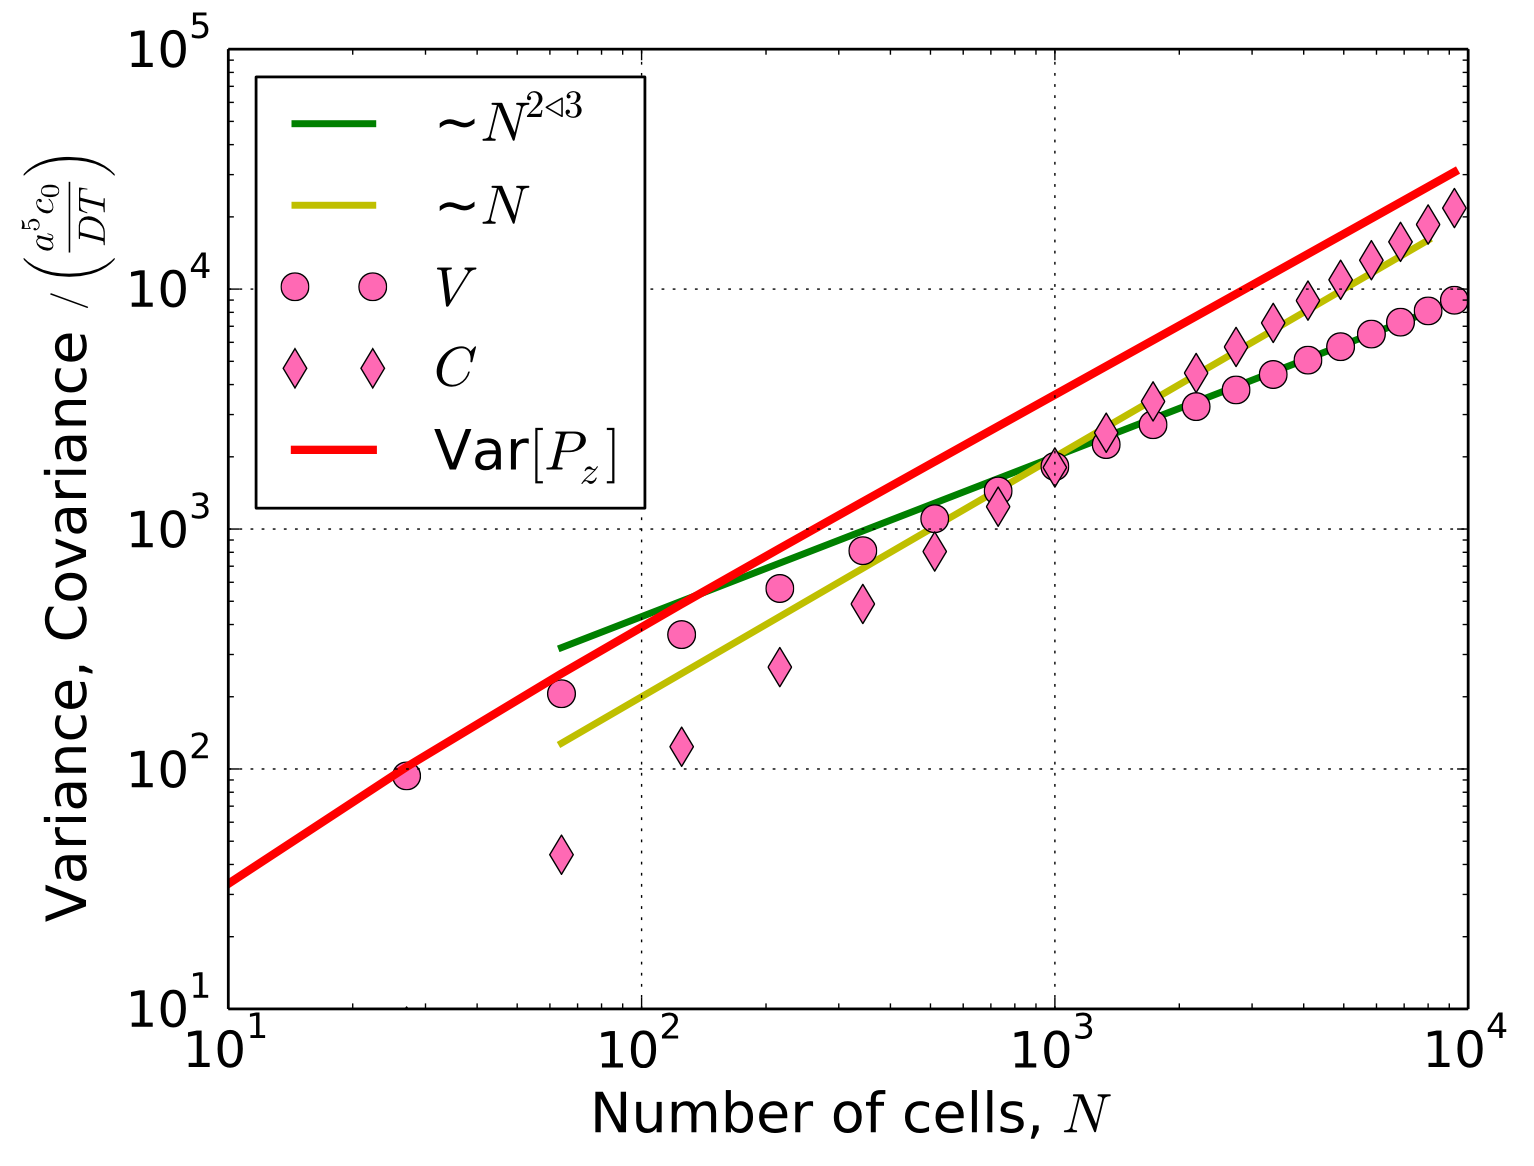
\includegraphics[width=0.8\textwidth]{../fig/ch3_si2.png}
    \caption{$\text{Var}[P_z]$ for a 3D cluster of EC cells. Cluster variance shown in red. Pink circles are the single cell variance contributions $V$, and pink diamonds are the cell-cell covariance contributions $C$.} \label{fig:ch3_4}
\end{figure}

The numerical results [Fig.\ \ref{fig:ch3_4}] show that $V \sim N^{2/3}$ since the number of edge cells also scales as $N^{2/3}$. We also find that $C \sim N$; the covariance contribution to the total cluster polarization grows linearly with $N$. For large clusters the $N$ scaling dominates the behavior of $\text{Var}[P_z]$. Therefore, in 3D the leading order scaling for the variance is
$\text{Var}[P_z] \sim N$ as in Table I of the main text.


% \section{Testing Analytic Model Assumptions}
%
% \begin{figure}[ht]
%     \centering
%         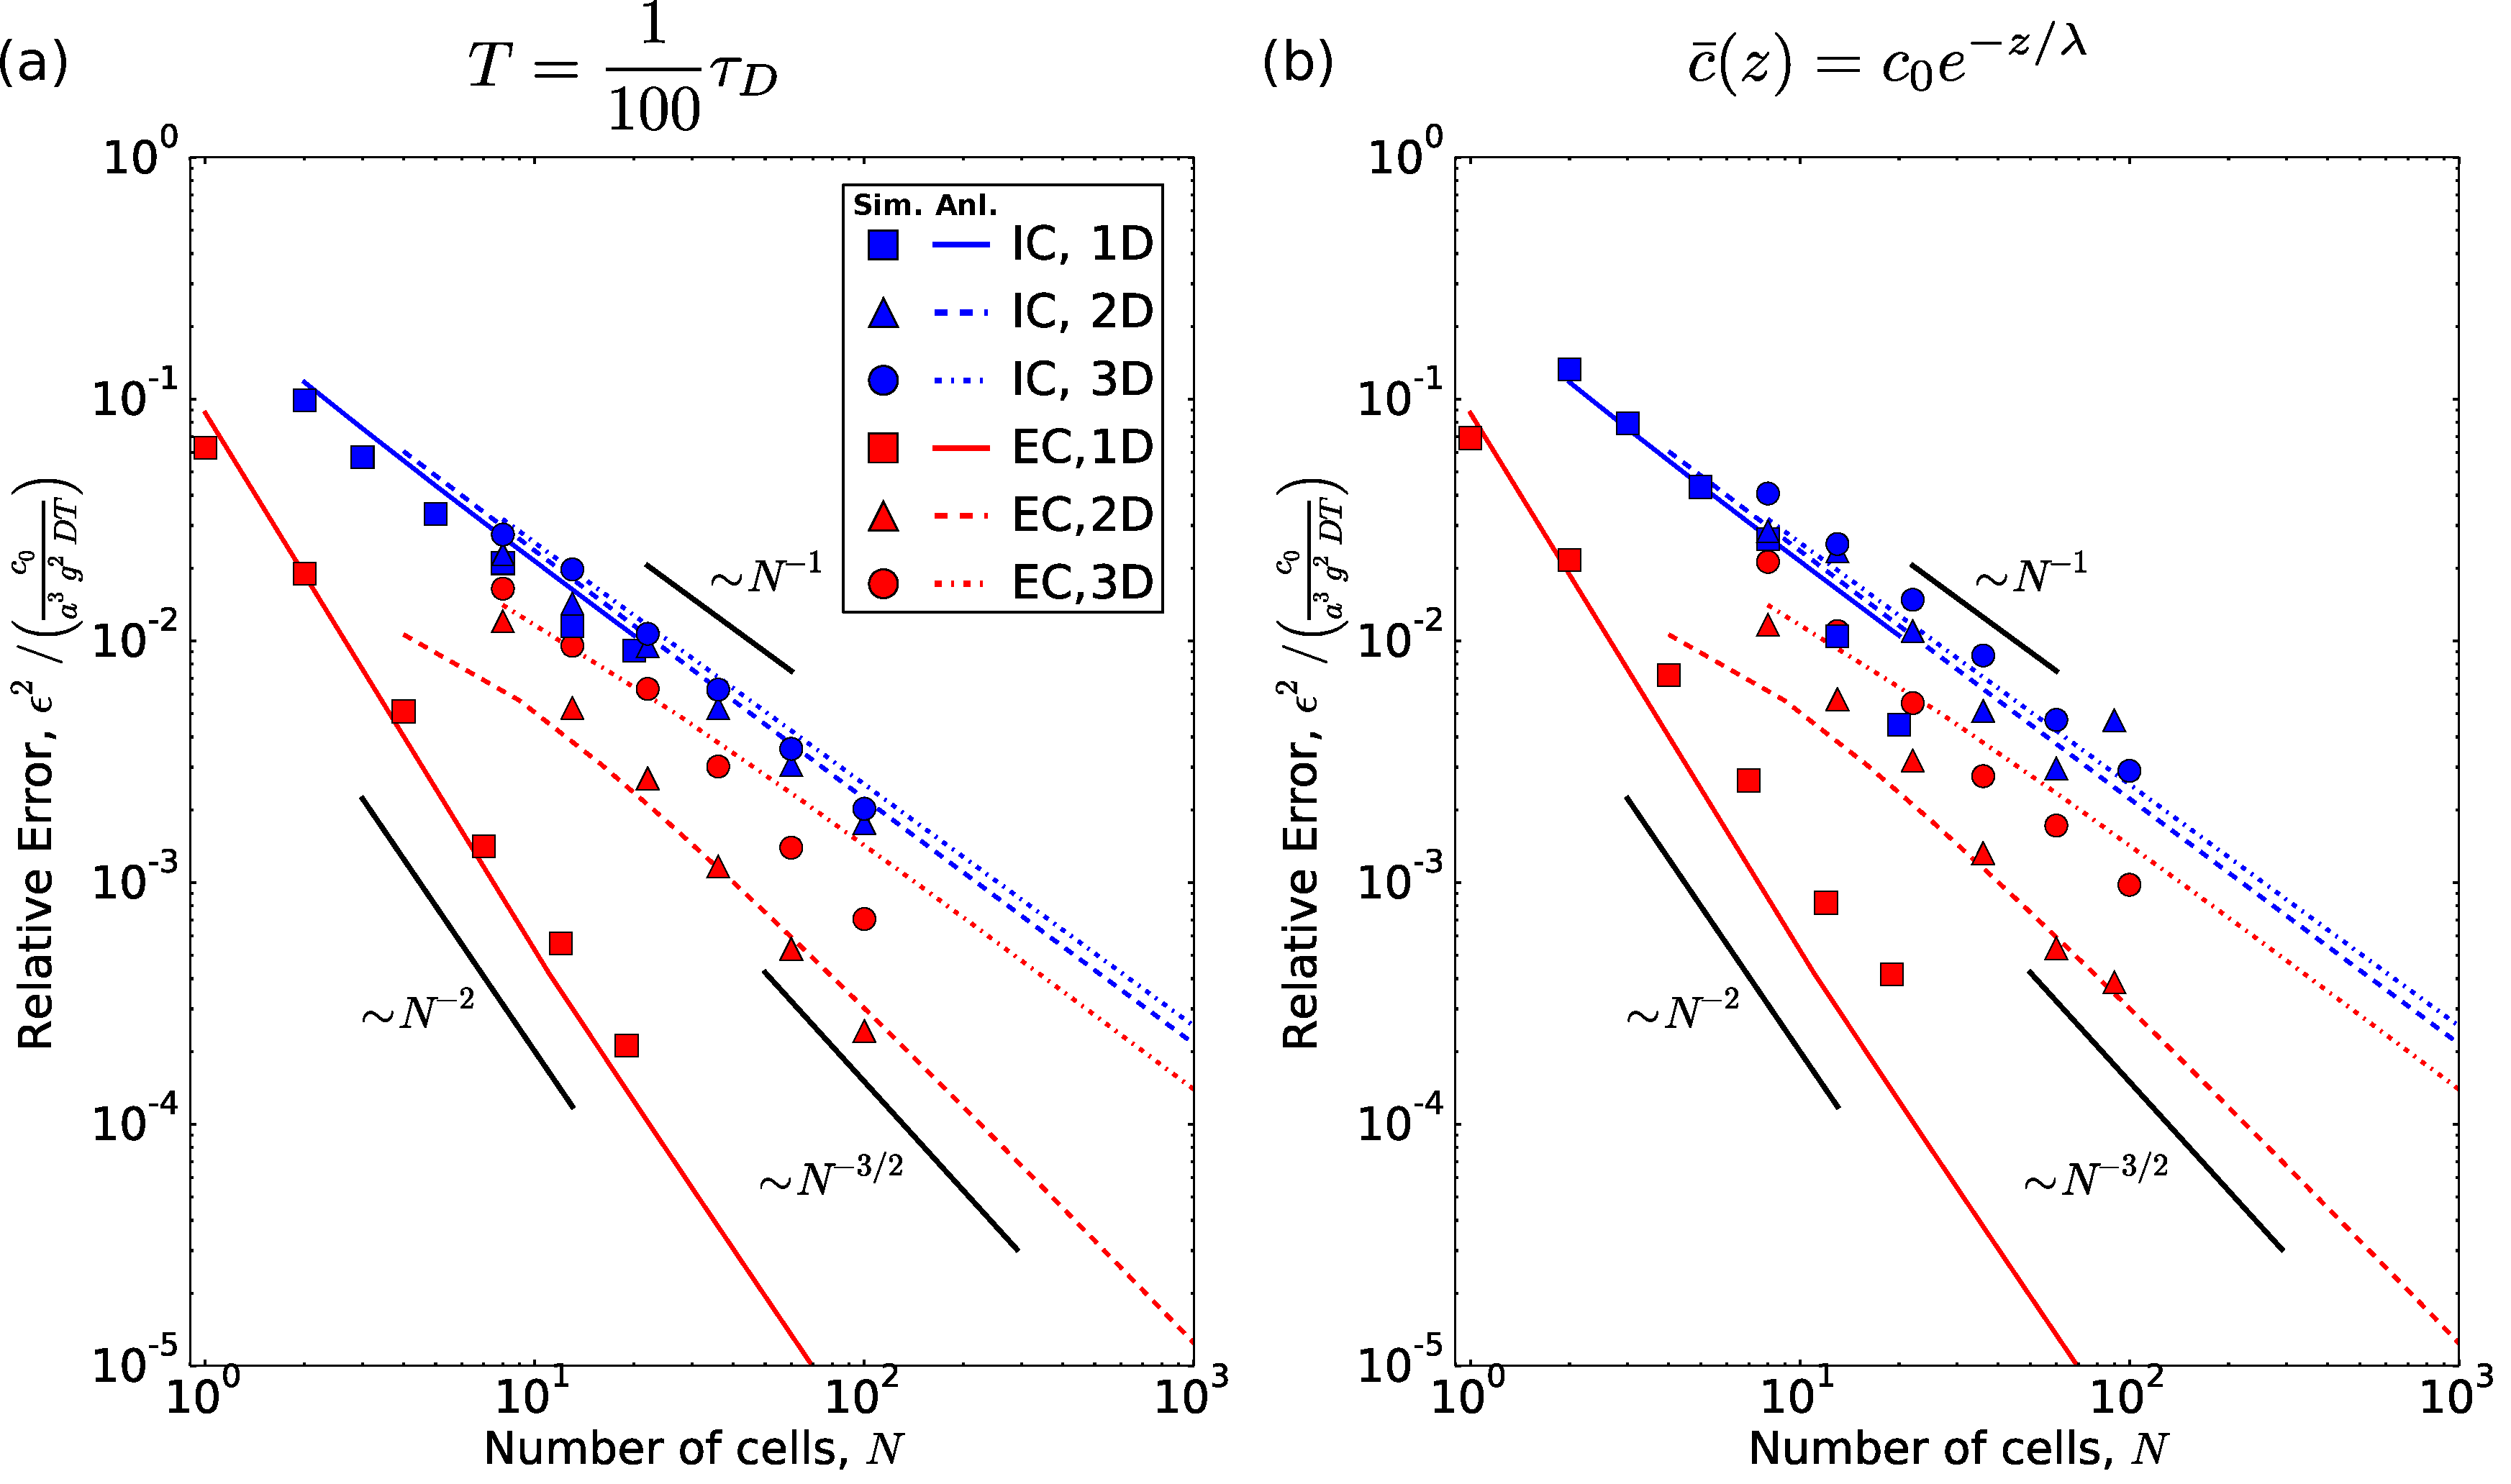
\includegraphics[width=0.8\textwidth]{../fig/ch3_si1.pdf}
%     \caption{(a) Short-time integration relative error results. Data points are of simulations for $T= \frac{1}{100} \tau_D$. (b) Exponential concentration profile relative error results. The mean concentration profile is $\bar{c}(z) = c_0 e^{-z/\lambda}$, the lengthscale $\lambda=\sqrt{D/\beta}$ is set by the diffusion coefficient $D$ and the molecule decay rate $\beta$. Lines are from original analytical predictions using $T > \tau_D$ and a linear concentration profile.} \label{fig:ch3_3}
% \end{figure}

% Simulations are performed to test model behavior when assumptions used to derive analytic results are relaxed. In Fig.\ \ref{fig:ch3_3}(a) we relax the assumption that the integration time $T$ must be larger than the timescale for diffusion $\tau_D \sim R^2/D$. We find that $\epsilon^2$ scales the same way as previously predicted for both EC and IC, even when $T = \tau_D/100$. The only exception is that $\epsilon^2$ for 3D EC [Fig.\ \ref{fig:ch3_3}(a), red circles] has a more negative power-law dependence on $N$ than the expected $\sim N^{-1}$. The shorter integration time results in decreased correlations between edge cells which when $T>\tau_D$ results in $C\sim N$. Hence with
% $T < \tau_D$
% the total variance is less dependent on $C$, and $V \sim N^{2/3}$ becomes the dominant contribution to $\text{Var}[P]$. This results in a steeper scaling of $\epsilon^2$ closer to
% $\text{Var}[P]/\langle P \rangle^2 \sim N^{2/3}/N^2 = N^{-4/3}$.
% Interestingly, we see that relaxing the assumption $T \gg \tau_D$ results in improved precision for EC over IC not just in 1D and 2D but also in 3D configurations.
%
% In Fig.\ \ref{fig:ch3_3}(b) we change the concentration profile from linear to exponential which has a mean concentration of
% $\bar{c}(z) = c_0 e^{-z/\lambda}$.
% The lengthscale $\lambda=\sqrt{D/\beta}$ depends on the diffusion coefficient and the molecule degradation rate $\beta$. In Fig.\ \ref{fig:ch3_3}(b) the simulation results are for $\lambda > a$. We find that $\epsilon^2$ is in very good agreement with our original analytic predictions. The only exception is that due to the exponential profile, $\langle P \rangle$ for 1D EC (Fig.\ \ref{fig:ch3_3}(b), red squares) is non-linear in $N$ causing the relative error data to scale less steeply than the expected $N^{-2}$.



\chapter{Dynamics of Collective Chemotaxis}

In this chapter we study the dynamics of more detailed model of collective emergent chemotaxis (EC) than that presented in Ch.\ 3. In this model we explicitly account for the following effects: cell-cell contact interactions, intercellular communication, individual cell motility, and cell size and shape fluctuations. This provides a more realistic application of the EC model presented in Ch.\ 3 with the addition of cell-cell communication in order to achieve adaptive gradient sensing across a whole collective of cells. The work discussed in this chapter has been published in \textit{Biophysical Journal} \cite{varennes2016collective}.

Cells can migrate in response to a chemoattractant and can detect extraordinarily small changes in chemical concentrations. The limits to cell sensory precision have been a topic of research in biology and biophysics for many years. \textit{Escheria coli} bacterial chemotaxis operates very near the physical limits of their sensory machinery, and \textit{Dictyostelium discoideum} amoebae are sensitive to differences in chemical concentrations on the order of ten molecules across the cell \cite{berg1977physics,song2006dictyostelium}. Recent studies on individual breast cancer cells showed that they are sensitive to 1\% differences in concentration across the cell length \cite{shields2007autologous}. Limits to cell sensory precision were first derived by Berg and Purcell almost 40 years ago \cite{berg1977physics} and have been revisited to account for binding kinetics, spatiotemporal correlations and spatial confinement \cite{bialek2005physical, kaizu2014berg, bicknell2015limits}. However, in nature cells are rarely found alone, and the interactions between nearby cells may alter cells' sensory capabilities.

In many biological contexts cells act in close proximity to one another which can have significant effects on collective behavior. Clusters of mammary epithelial cells, lymphocytes and neural crest cells can detect chemical gradients that single cells cannot \cite{ellison2016cell,malet2015collective,theveneau2010collective}, and cultures of neurons have been shown to be sensitive to single molecule differences across an individual neuron's axonal growth cone \cite{rosoff2004new}.
In many types of cancer, tumor cell invasion is collective, involving coherent grouped motion guided by chemical cues \cite{cheung2013collective, friedl2012classifying, aceto2014circulating, puliafito2015three}. It is clear from these examples that cells acting collectively can improve upon their individual sensory precision.
Similar to the limits set by Berg and Purcell, the physical limits to collective gradient sensing have been recently derived \cite{mugler2016limits,ellison2016cell} by using a multicellular version of the local excitation-global inhibition (LEGI) communication model \cite{levchenko2002models}, one of the simplest adaptive mechanisms of gradient sensing. With these studies the physical limits of cell sensing have been extended from single cells to multicellular collectives.

In parallel to research on cell sensory precision, studies on collective cell  migration have also advanced. Biological processes such as development, cellular migration, pathogenic response, and cancer progression all involve many cells acting in a coordinated way \cite{scarpa2016collective,friedl2010plasticity,rasmussen2006quorum,boelens2014exosome,cheung2013collective,vader2014extracellular,szabo2016modelling}. Simple mechanical models successfully explain observed collective behaviors such as cell streaming, cell sorting, cell sheet migration, wound healing, and cell aggregation \cite{kabla2012collective,szabo2010collective,basan2013alignment,janulevicius2015short}. These models accurately model collective cell migration but fail to explicitly include the affects of multicellular sensing in driving the mechanics at play. Cells are often capable of intercellular communication, so understanding how communicated information is translated into mechanical action is of prime interest.

How the phenomena of collective sensing and multicellular migration are connected remains an open question \cite{varennes2016sense,defranco2008migrating,haeger2015collective}. Recent studies by Camley et al.\ \cite{camley2016emergent} and Malet-Engra et al.\ \cite{malet2015collective} have started to address this need for modeling collective sensing and migration. In the study of Camley et al.\ individual cell measurements act to polarize cells in a cluster outwards causing tension, and when intercellular communication is added the tension on the cluster adapts to the chemical concentration. Both studies do not take into account the inherent stochasticity of cell sensing and intercellular communication. However, individual cell measurements of the environment are error-prone while propagation of single cell measurements also adds noise to the system. These studies also treat cells or clusters as perfect circles, neglecting natural geometric fluctuations in the size and shapes of cells that occur during migration.

Here we focus our attention on stochastic processes governing collective gradient sensing and cell motility. First, the limits to collective gradient sensing are briefly reviewed and our implementation of multicellular LEGI described. Information gained from collective sensing then must be used to direct cell motion. We develop a model which takes into account the fluctuating shape of cells while coupling cell motility to noisy collective gradient sensing. We model intercellular communication via the direct exchange of messenger molecules between cells. Candidate mediators of such intercellular communication have been recently identified in \textit{Drosophila} development \cite{ramel2013rab11}, and other studies suggest intercellular communication's involvement in organoid branching, angiogenesis, and cancer \cite{ellison2016cell,gerhardt2003vegf,hsu2000cadherin,friedl2009collective}. We study cluster migration in shallow gradients where the change in concentration across a cell width is very small relative to the background concentration. This regime is of prime interest since experiments show that collectives can respond to these shallow gradients whereas single cells cannot \cite{ellison2016cell,malet2015collective,rosoff2004new}. By explicitly modeling the stochastic processes of sensing and migration this model places constraints on the collective behavior of cells and predicts an optimal cluster size for fastest chemotaxis. We conclude by discussing our model's implications for cell migration experiments.


\begin{figure}
    \centering
        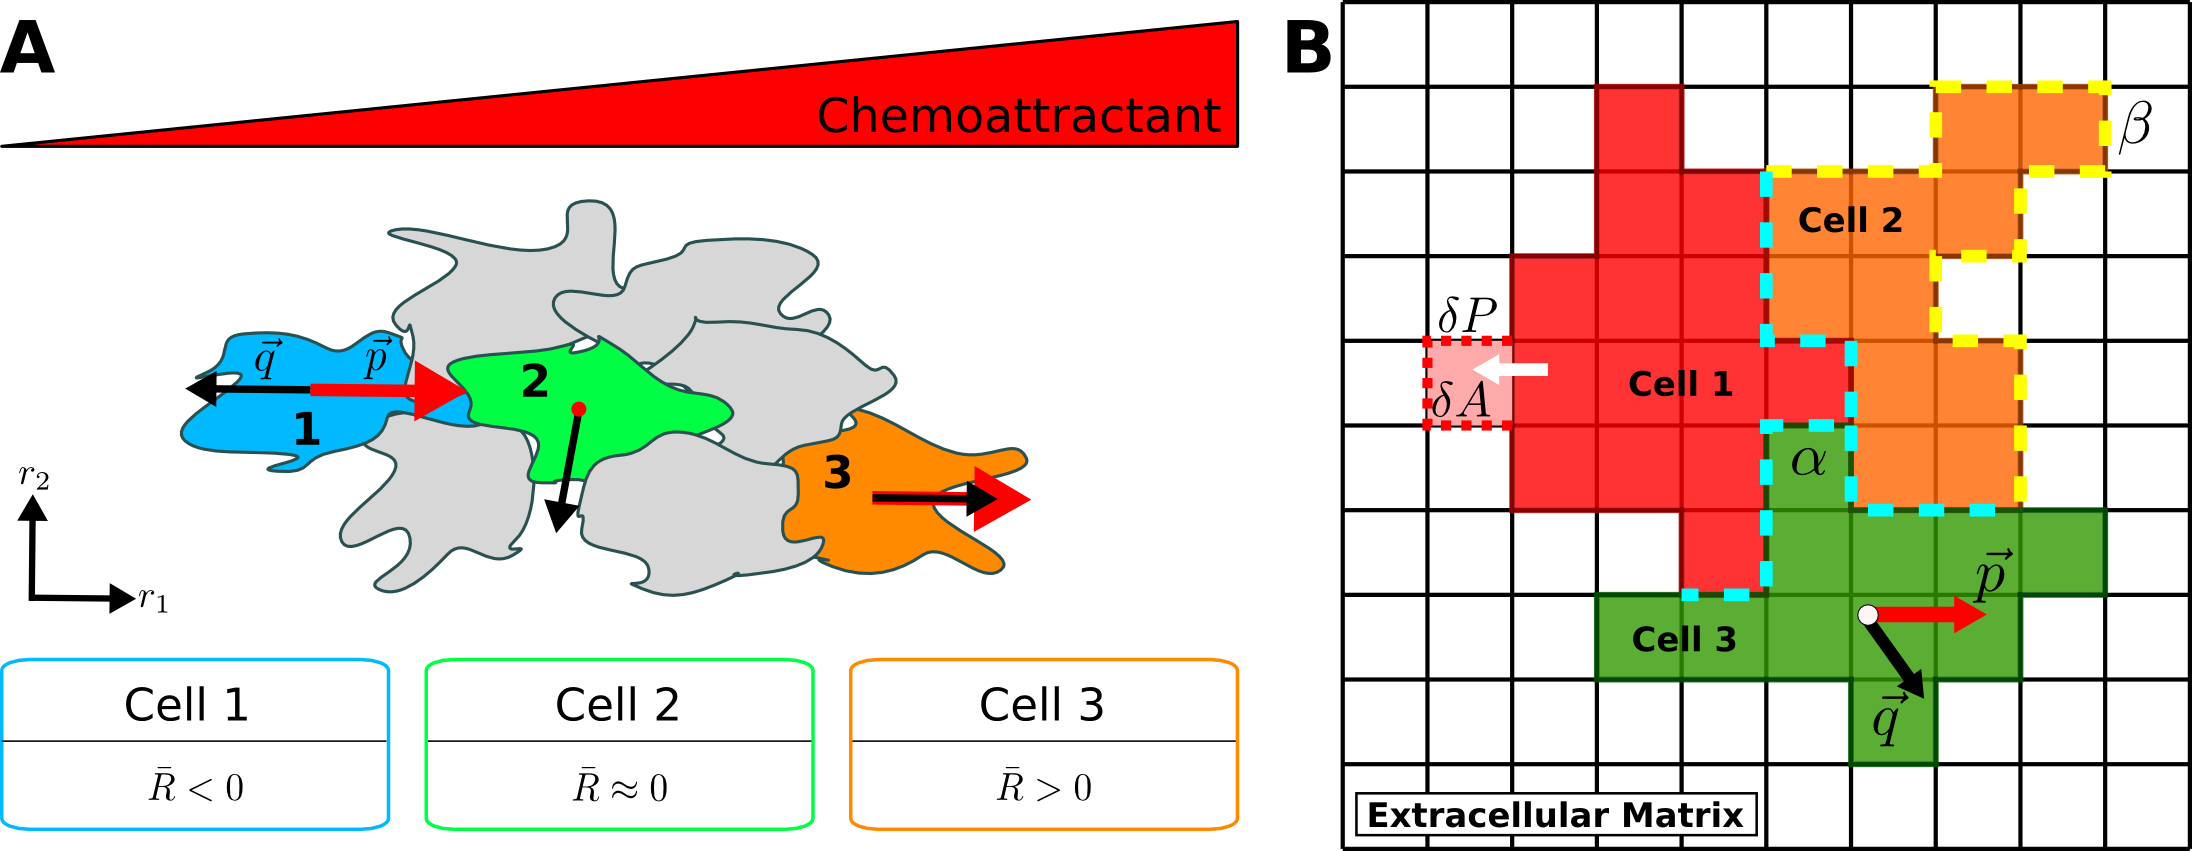
\includegraphics[width=0.80\textwidth]{../fig/ch4_fig1.png}
    \caption{Model implementation. (A) Cell polarization is biased by multicellular sensing. On average, the cells on the left and right edges will measure negative and positive values of $R$, respectively. This causes the left-edge (Cell 1) and right-edge (Cell 3) cells to polarize in the direction of the gradient, while cells in the middle (Cell 2) are on average not polarized since $\bar{R} \approx 0$. Polarization vectors $\vec{p}$ are red, repulsion vectors $\vec{q}$ are black. (B) Simulations are implemented using the Cellular Potts Model (CPM). Cells comprise of simply connected lattice points. There are adhesion energies associated with different types of contact: cell-cell, $\alpha$ (blue-dashed line), and cell-ECM, $\beta$ (yellow-dashed line). Cell motility is modeled by the addition/removal of lattice points (pink). Each cell has a center-of-mass (white dot), a polarization vector, $\vec{p}$ (red) and a repulsion vector, $\vec{q}$ (black).} \label{fig:model}
\end{figure}


\section{MODEL}

Communication between cells and collective sensing can improve upon an individual cell's ability to sense the environment \cite{ellison2016cell}, and in turn this information may be used to direct cell motion. To describe collective sensing, we will use the well-established local excitation--global inhibition (LEGI) mechanism \cite{mugler2016limits,levchenko2002models}.

\subsection{Limits to Multicellular Sensing}

Individual cells measure spatial gradients by comparing concentration measurements $c$ made by receptors or groups of receptors on the cell surface \cite{mugler2016limits,jilkine2011comparison}. For simplicity, we assume that a cell of size $a$ compares the number of diffusing molecules within two different regions of size $b$ which run parallel to the chemical gradient $\bar{g}$.
The relative error in each compartment's measurement is
$ \left(\sigma_c / \bar{c} \right)^2 \sim 1 / \left( b\bar{c}DT \right) $ \cite{berg1977physics},
where $D$ is the diffusion coefficient, and $T$ is the measurement integration time. Assuming that the measurements made in each compartment are independent, then the difference in counts is proportional to the gradient
$\Delta\bar{n} = \bar{n}_2 - \bar{n}_1 \sim ab^3\bar{g}$.
In the limit that the gradient is very small relative to the background concentration $a\bar{g}\ll\bar{c}$, the relative error in gradient sensing simplifies to
\begin{equation} \label{eq:g}
\frac{\sigma_g}{\bar{g}} = \frac{\sigma_{\Delta n}}{\Delta \bar{n}} \sim \sqrt{\frac{\bar{c}}{b(a\bar{g})^2DT}}.
\end{equation}
Eq.\ \ref{eq:g} has been extensively derived and generalized to systems with different geometries \cite{endres2008accuracy,endres2009accuracy,hu2010physical} and in all such cases a term of the form in Eq.\ \ref{eq:g} appears as the fundamental limit, with the length scale $b$ dictated by the particular sensory mechanism and geometry. In the case of multicellular gradient sensing, we consider the cells on opposite ends of a chain of cells as the two compartments comparing concentration measurements. Then in Eq.\ \ref{eq:g} $b \to a$ and $a \to Na$ where $N$ is the number of cells in the chain. The relative error for the multicellular cluster becomes \cite{mugler2016limits}
\begin{equation} \label{eq:G1}
\frac{\sigma_g}{\bar{g}} \sim \sqrt{\frac{\bar{c}}{a(Na\bar{g})^2DT}}.
\end{equation}
There is a crucial effect that is neglected in formulating Eq.\ \ref{eq:G1} which is the mechanism by which the cells communicate their measurements across the collective. Communication will introduce additional noise to the gradient sensing process thereby altering the expression for the relative error. In the case of a single cell it is reasonable to assume that measurements from different compartments can be reliably transmitted, but with the increased size of the multicellular cluster we cannot make the same assumption. Using the multicellular LEGI paradigm \cite{levchenko2002models} to model intercellular communication, the physical limits to communication-aided collective gradient sensing have been derived \cite{ellison2016cell, mugler2016limits}, which we expand upon below.

\subsection{Multicellular LEGI Model}

In the LEGI model cells produce two chemical species, a ``local'' species $X$, and a ``global'' species $Y$, in response to the chemoattractant $S$. The local species $X$ remains within an individual cell and represents that cell's measurement of its local chemical concentration. This species can be a molecule produced or activated in response to attractant-bound receptors, or the bound receptors themselves. The global species $Y$ can diffuse at the rate $\gamma$ between neighboring cells and therefore represents the average $X$ population among neighboring cells. $Y$ molecules may only be exchanged when two or more cells are in direct contact with one another. Recent experiments in epithelial cells identified this global species as either calcium or a small molecule involved in calcium signaling (such as IP3), and identified the intercell diffusion mechanism as mediated by gap junctions \cite{ellison2016cell}. Finally, $X$ activates a downstream reporter molecule $R$, while $Y$ inhibits $R$.

Let $x_k$, $y_k$, and $R_k$ represent the molecule populations in $X$, $Y$, and $R$ in the $k^\text{th}$ cell. The chemical reactions in cell $k$ are
\begin{equation}
    \begin{aligned}
        s_k &\xrightarrow{\kappa} s_k + x_k \hspace{20pt} x_k \xrightarrow{\mu} \emptyset \\
        s_k &\xrightarrow{\kappa} s_k + y_k \hspace{20pt} y_k \xrightarrow{\mu} \emptyset \hspace{20pt} y_k \rightleftharpoons_{\gamma_{j,k}}^{\gamma_{k,j}} y_{j} .
    \end{aligned}
\end{equation}
The production and degradation rates for $X$ and $Y$ are $\kappa$ and $\mu$, respectively. The global reporter molecule exchange rate $\gamma$ is dependent on the length of the interface $\mathcal{C}$ made between adjacent cells, and on the exchange rate per unit contact-length $\Gamma$,
$$\gamma_{j,k} = \int_{\mathcal{C}} \Gamma dl . $$
In the limit of strong communication ($\gamma \gg \mu$) and many cells, the relative error of gradient sensing is limited from below by \cite{mugler2016limits}
\begin{equation} \label{eq:G2}
\frac{\sigma_g}{\bar{g}} \sim \sqrt{\frac{\bar{c}}{a(n_0a\bar{g})^2DT}},
\end{equation}
where $n_0$ sets an effective number of cells over which information can be reliably conveyed. In our model communication between cells improves with increased diffusion of $Y$ molecules and so $n_0^2 \propto \gamma/\mu$ \cite{ellison2016cell, mugler2016limits}. As collectives grow larger than $n_0$ cells the relative error ceases to improve, saturating to the limit set by Eq.\ \ref{eq:G2}; unlike Eq.\ \ref{eq:G1} where the effects of communication are ignored and the relative error decreases without bound.

In the limit of shallow gradients, which are of primary interest in studying collective sensing, $R$ effectively reports the difference in $X$ and $Y$ molecule populations \cite{ellison2016cell} and so we will model the downstream readout as $R_k = x_k-y_k$. A negative (positive) difference indicates that the cell is below (above) the average measured concentration relative to nearby cells as shown by the reported average $R$ values for each cell in Fig.\ \ref{fig:model}A.

The chemical concentration is modeled as a space-dependent field $E(r_1,r_2)$, and in this case has a constant gradient in the $r_1$-direction,
\begin{gather*}
    E(r_1,r_2) = \bar{g}r_1 + \bar{c}.
\end{gather*}
The average signal in the $k^\text{th}$ cell's local environment is $\bar{s}_k = \int_{A_k} dr_1 dr_2 \ E(r_1,r_2)$ where $A_k$ is the area of the $k^\text{th}$ cell. Since diffusion is a Poisson process the variance in the measured signal $s_k$ is equal to the mean, $\sigma_{s_k}^2 = \bar{s}_k$. At each time step we sample $s_k$ for each cell from a Gaussian distribution with mean and variance $\bar{s}_k$, which corresponds to instantaneous sensory readout \cite{ellison2016cell}. The dynamics of the local reporter satisfy the stochastic differential equation
\begin{equation} \label{eq:xdot}
    \dot{x}_k = \kappa s_k - \mu x_k + \eta_{x_k}.
\end{equation}
The first term in Eq.\ \ref{eq:xdot} is due to the production of $X$ molecules due to the signal $S$, the second term represents molecule degradation, and the third term $\eta_{x_k}$ accounts for the noise inherent to these reactions. The noise term is equal to
$\eta_{x_k} = \sqrt{\kappa\bar{s}_k}\xi_{1,k} - \sqrt{\mu \bar{x}_k} \xi_{2,k}$ since both production and degradation are stochastic processes \cite{gillespie2000chemical}.
In Eq.\ \ref{eq:xdot} and subsequent stochastic equations $\xi_{i,k}$ and $\chi_{j,k}$ are unit Gaussian random variables representing the noise in molecule populations. For the local reporter, the steady-state solution is simply
\begin{equation} \label{eq:xss}
    x_{k}^{ss} = \left( \kappa/\mu \right) s_k + \left( 1/\mu \right) \eta_{x_k}.
\end{equation}

The dynamics of the global species can be modeled in similar fashion,
\begin{equation} \label{eq:ydot}
    \dot{y}_k = \kappa s_k - \mu y_k - y_k \sum_{\langle j,k \rangle} \gamma_{j,k} + \sum_{\langle j,k \rangle} y_j \ \gamma_{j,k} + \eta_{y_k} .
\end{equation}
The first summation term in Eq.\ \ref{eq:ydot} accounts for the loss of $y_k$ due to the diffusion out to neighboring cells, and similarly the second summation term accounts for the increase in $y_k$ due to diffusion into cell $k$ from its neighbors. The notation $\langle j,k \rangle$ represents the set of all nearest neighbor pairs. The noise term $\eta_{y_k}$ in the molecule dynamics depends on the production, degradation and diffusion of $Y$ molecules. In steady-state we can express the noise as
\begin{equation*}
    \eta_{y_k} = \sqrt{\kappa \bar{s}_k} \xi_4 - \sqrt{\mu\bar{y}_k} \xi_5 + \sum_{j=1}^N \left[ \chi_{j,k} \sqrt{\gamma_{j,k}} \left( \sqrt{\bar{y}_j}-\sqrt{\bar{y}_k} \right) \right] .
\end{equation*}
Similarly to $\eta_{x_k}$, the noise in $y_k$ also depends on production and degradation while an extra term is required to account for the noise in $Y$ molecule exchange. Eq.\ \ref{eq:ydot} can be simplified by noting that exchange rates between cells are symmetric $\gamma_{j,k}=\gamma_{k,j}$, $\gamma_{i,i}=0$, and by defining the sum of all the exchange rates between cell $k$ and all other cells as $G_k = \sum_{j=1}^N \gamma_{j,k}$. The steady-state solution for the global reporter is more involved than the local reporter, and can be written as a matrix equation
\begin{equation} \label{eq:yss}
    M\vec{y}^{ss} = \kappa\vec{s} + \vec{\eta}_y,
\end{equation}
where $M$ is a square, symmetric matrix that governs the degradation and exchange of $Y$ molecules in all cells,
\begin{equation} \label{eq:Mmatrix}
    M =
    \begin{bmatrix}
     \mu+G_1 & -\gamma_{1,2} & \cdots & -\gamma_{1,N} \\
     -\gamma_{2,1} & \mu+G_2 & \cdots & -\gamma_{2,N} \\
     \vdots  & \vdots  & \ddots & \vdots  \\
     -\gamma_{N,1} & -\gamma_{N,2} & \cdots & \mu+G_N
    \end{bmatrix}.
\end{equation}


\begin{table}[b]
\centering
\footnotesize
\begin{tabular}{ |c|c|c| }
\hline
Parameter & Value & Notes \\ \hline
Concentration $\bar{c}$ & $10 \text{nM}$ & Assumes $\bar{c} \gg a\bar{g}$ for shallow gradients \cite{malet2015collective,ellison2016cell} \\
Gradient $\bar{g}$ & $0.04 \text{nM/}\mu\text{m}$ & \\ \hline
LEGI Molecule Production Rate $\kappa$ & $19.72 \text{min}^{-1}$ & Assumes $ \{\kappa,\mu\} \gg r$ \\
LEGI Molecule Degradation Rate $\mu$ & $19.72 \text{min}^{-1}$ & i.e.\ biochemical signaling is faster than motility response \\ \hline
Global Reporter Exchange Rate $\Gamma$ & $80 (\mu\text{m} \ \text{min})^{-1}$ & Varied in Fig.\ \ref{fig:results} \\ \hline
Polarization Bias Strength $\epsilon$ & 0.8 & Varied in Fig.\ \ref{fig:heat} \\ \hline
Polarization Decay Rate $r$ & $3.94 \text{min}^{-1}$ & Sets polarization memory time, as used in \cite{szabo2010collective} \\ \hline
Relaxed Cell Area $A_0$ & $315 \mu\text{m}^2$ & Assumes cell radius $10 \mu\text{m}$ \cite{leber2009molecular} \\ \hline
Relaxed Cell Perimeter $P_0$ & $3.6\sqrt{A_0} \mu\text{m}$ & Assumes circular resting shape \\ \hline
Cell-cell Contact Energy $\alpha$ & 1.0 & Sets energy scale \\
Cell-ECM Contact Energy $\beta$ & 3.5 & $2\beta > \alpha$ for cell adhesion \cite{graner1992simulation} (Varied in Fig.\ \ref{fig:heat}) \\ \hline
Area Energy Cost $\lambda_A$ & 1.5  & Prevents ``stringy'' cell-shapes \\
Perimeter Energy Cost $\lambda_P$ & 0.01 & \\ \hline
\end{tabular}
\caption{Table of parameter values. Energy costs are in units of $k_B T$, where $k_B T$ is the thermal energy of the CPM Monte Carlo scheme.}
\label{table:ch4_1}
\end{table}


\subsection{Connecting Gradient Sensing to Cell Motility}

To describe collective migration, we integrate the output of multicellular LEGI gradient sensing with cell motility. Cells in motion have a distinct front and are polarized along the direction of the front to back. Cells within the cluster have their polarization biased by a combination of the LEGI readout and intercellular repulsion due to contact inhibition of locomotion (CIL). CIL is the phenomenon where cells that come into contact cease to form protrusions in the direction of contact \cite{mayor2010keeping}. This is a very simple way for cells to translate the noisy, error-prone gradient measurements into collective cell motility \cite{camley2016emergent,malet2015collective,theveneau2010collective}.

In order to connect sensing to motility, we couple individual cell polarization $\vec{p}$ to both the LEGI downstream readout $R$ and what we will call the cell's repulsion vector $\vec{q}$. The cell's polarization vector represents the desired direction of motion \cite{jilkine2011comparison} and modeling collective behavior using cell polarization has been done previously\cite{szabo2010collective,camley2016emergent}. Information about the cell's surroundings are naturally expressed by the repulsion vector $\vec{q}$ \cite{camley2016emergent}. The repulsion vector is representative of contact inhibition of locomotion (CIL) \cite{mayor2010keeping}. CIL demonstrates that cells are aware of their immediate surroundings. The repulsion vector for cell $k$ is a unit vector that points away from all of cell $k$'s neighbors.
\begin{equation}
    \vec{q}_k = \left( \frac{1}{\sum_{\langle j,k \rangle} L_{j,k}|\vec{x}_k - \vec{x}_j|} \right)
    \sum_{\langle j,k \rangle} L_{j,k} \left( \vec{x}_k - \vec{x}_j \right),
\end{equation}
where $L_{j,k}$ is the contact length made between cell $k$ and its neighboring cell $j$. In our model cell polarization will change as a function of time depending on a combination of the repulsion vector and the LEGI downstream readout,
\begin{equation} \label{eq:polarVec}
    \frac{d\vec{p}_k}{dt} = r \left[ -\vec{p}_k + \epsilon \frac{R_k}{\sigma_R} \vec{q}_k \right].
\end{equation}
The first term in Eq.\ \ref{eq:polarVec} models the decay of cell polarization. In the absence of any stimulus an individual cell will undergo a persistent random walk with a timescale $1/r$ \cite{szabo2010collective}. The second term acts to align or anti-align the cell’s polarization vector with the repulsion vector, with alignment strength $\epsilon$ based on the cell's readout $R_k$. The magnitude of $R_k$ is normalized by its standard deviation $\sigma_R$. The net effect is illustrated in Fig.\ \ref{fig:model}A.

In the presence of a gradient, cells on the edge near the lower-end of the chemical concentration will tend to be polarized into the cluster (Cell 1 in Fig.\ \ref{fig:model}A), whereas cells on the higher concentration edge tend to be polarized outwards (Cell 3 in Fig.\ \ref{fig:model}A). Cells in the center of the cluster (Cell 2 in Fig.\ \ref{fig:model}A) are on average unpolarized. The net effect is that the cells on the edges of the cluster will drive motion in the direction of increasing chemical concentration. It is important to note that in this model single cells are unable to chemotax since the multicellular LEGI mechanism requires more than one cell to detect a gradient, and similarly without neighboring cells there is no repulsion vector to bias the cell's polarization.


\subsection{Computational Implementation}

Computational simulations are conducted in order to understand the dynamics that evolve from the model of collective sensing and migration. The source code for the simulations can be found here \cite{ch2code}. The implementation chosen is the Cellular Potts Model (CPM) \cite{graner1992simulation,swat2012multi} although other cellular automata models are possible as well \cite{ermentrout1993cellular,maire2015molecular,mente2015analysis}. The CPM is widely used for simulating cell-centric systems. Despite its relative simplicity, this computational implementation can qualitatively reproduce diverse biological phenomena \cite{maree2007cellular}. The CPM is a very good implementation for simulating systems wherein cell geometry is crucial to the dynamics of the system. Using CPM many studies, some involving cell polarization and mechanical-based coupling, successfully reproduce epithelial cell streaming, cell sorting, chemotaxis and collective migration \cite{maclaren2015models,kabla2012collective,szabo2010collective}.

In the CPM cells exist on a discrete lattice and are represented as groupings of lattice points. Simply-connected groups of lattice sites $x$ with the same integer values for their \textit{lattice label} $\sigma(x)>0$ comprise a single cell. The extracellular matrix (ECM) is labeled with the lattice label $\sigma(x)=0$. Cells have a desired size and perimeter from which they can fluctuate, and cells adhere to their neighboring environment with an associated adhesion energy. The energy of the whole system is the sum of contributions from adhesion $J_{i,j}$, area-restriction $\lambda_A$, and perimeter-restriction $\lambda_P$ terms,
\begin{equation}
    u = \sum_{\langle x,x' \rangle} J_{\sigma(x),\sigma(x')} + \sum_{i=1}^N \left( \lambda_A (\delta A_i)^2 + \lambda_P (\delta P_i)^2 \right),
\end{equation}
\begin{equation}
    J_{\sigma(x),\sigma(x')} =
    \begin{cases}
        0 &\sigma(x)=\sigma(x') \ \text{(within the same cell)}, \\
        \alpha &\sigma(x)\sigma(x')>0 \ \text{(cell-cell contact)}, \\
        \beta &\sigma(x)\sigma(x')=0 \ \text{(cell-ECM contact)}.
    \end{cases}
\end{equation}
The parameters $\alpha$ and $\beta$ characterize intercellular adhesiveness, and in order to ensure that it is energetically favorable for cells to remain in contact, we restrict $\beta > 2\alpha$ \cite{szabo2010collective}. $\beta$ represents the cell-ECM contact energy, a larger value corresponds to an ECM that is more difficult to traverse. Heterogeneities in the microenvironment could be represented by a spatially dependent $\beta$; here we take $\beta$ to be a constant. The area- and perimeter-restriction energy terms prevent cells from growing or shrinking to unphysical sizes as well as branching or stretching into unphysical shapes. Cells fluctuate in shape and size around the desired area $A_0$ and perimeter $P_0$ with $\delta A_i \equiv A_i-A_0$ (and similarly for $\delta P_i$). The resulting dynamics evolve from the minimization of the system's energy under thermal fluctuations.

Cell dynamics are a consequence of minimizing the energy of the whole system. This is a random process that is sensitive to thermal fluctuations and is modeled using a Monte Carlo process. In a system of $n$ lattice sites, one \textit{Monte Carlo} time step (MC step) is composed of $n$ \textit{elementary} steps. Each elementary step consists of an attempt to copy the lattice label of a randomly chosen lattice site onto that of a randomly chosen neighboring site as illustrated by the pink lattice site in Fig.\ \ref{fig:model}B. The new configuration resulting from the copy is accepted with probability $P$, which depends on the change in the system's energy accrued in copying over the lattice label,
\begin{equation} \label{eq:prob}
    P =
    \begin{cases}
        e^{-\left( \Delta u - w \right)} &\ \Delta u - w > 0 , \\
        1 &\ \Delta u - w \leq 0 .
    \end{cases}
\end{equation}
The term $\Delta u$ is the change in energy of the system due to the proposed lattice label copy. $w$ is the \textit{bias} term which acts to bias cell motion in the direction of polarization. The bias term in the CPM model is required in order for cell clusters to exhibit directed motion \cite{szabo2010collective},
\begin{equation} \label{eq:w}
    w = \sum_{k=\sigma(a),\sigma(b)} \frac{\Delta\vec{x}_{k(a \to b)} \cdot \vec{p}_k}{ |\Delta\vec{x}_{k(a \to b)}| |\Delta\vec{x}_{k(\Delta t)}|}.
\end{equation}
The summation in Eq.\ \ref{eq:w} is over the cells involved in the elementary time step: $a$ is the lattice site being copied, and $b$ is the lattice site being changed. The change in the cell's center of mass position during the elementary time step is $\Delta\vec{x}_{k(a \to b)}$, whereas $\Delta\vec{x}_{k(\Delta t)}$ is the cell's change in the center of mass during a MC step. The cell polarization vector $\vec{p}_k$ is updated at every MC step in accordance with Eq.\ \ref{eq:polarVec}. The dot product acts to bias cell motion since movement that is parallel to the polarization vector will result in a more positive $w$ which in turn results in a higher acceptance probability (Eq.\ \ref{eq:prob}).

In addition to calculating the energy of the system, at each MC step the $X$ and $Y$ molecule populations in each cell are sampled by solving Eq.\ \ref{eq:xss} and \ref{eq:yss}. In doing so our model accounts for fluctuations in molecule numbers, cell shape, and cell-cell contact. With this computational implementation cells on the edges of the cluster are polarized in the direction of increasing chemical concentration, and cells near the center of the cluster have no net polarization, resulting in collective migration in the direction of increasing chemical concentration.


\section{Results}


\begin{figure}[ht]
    \centering
        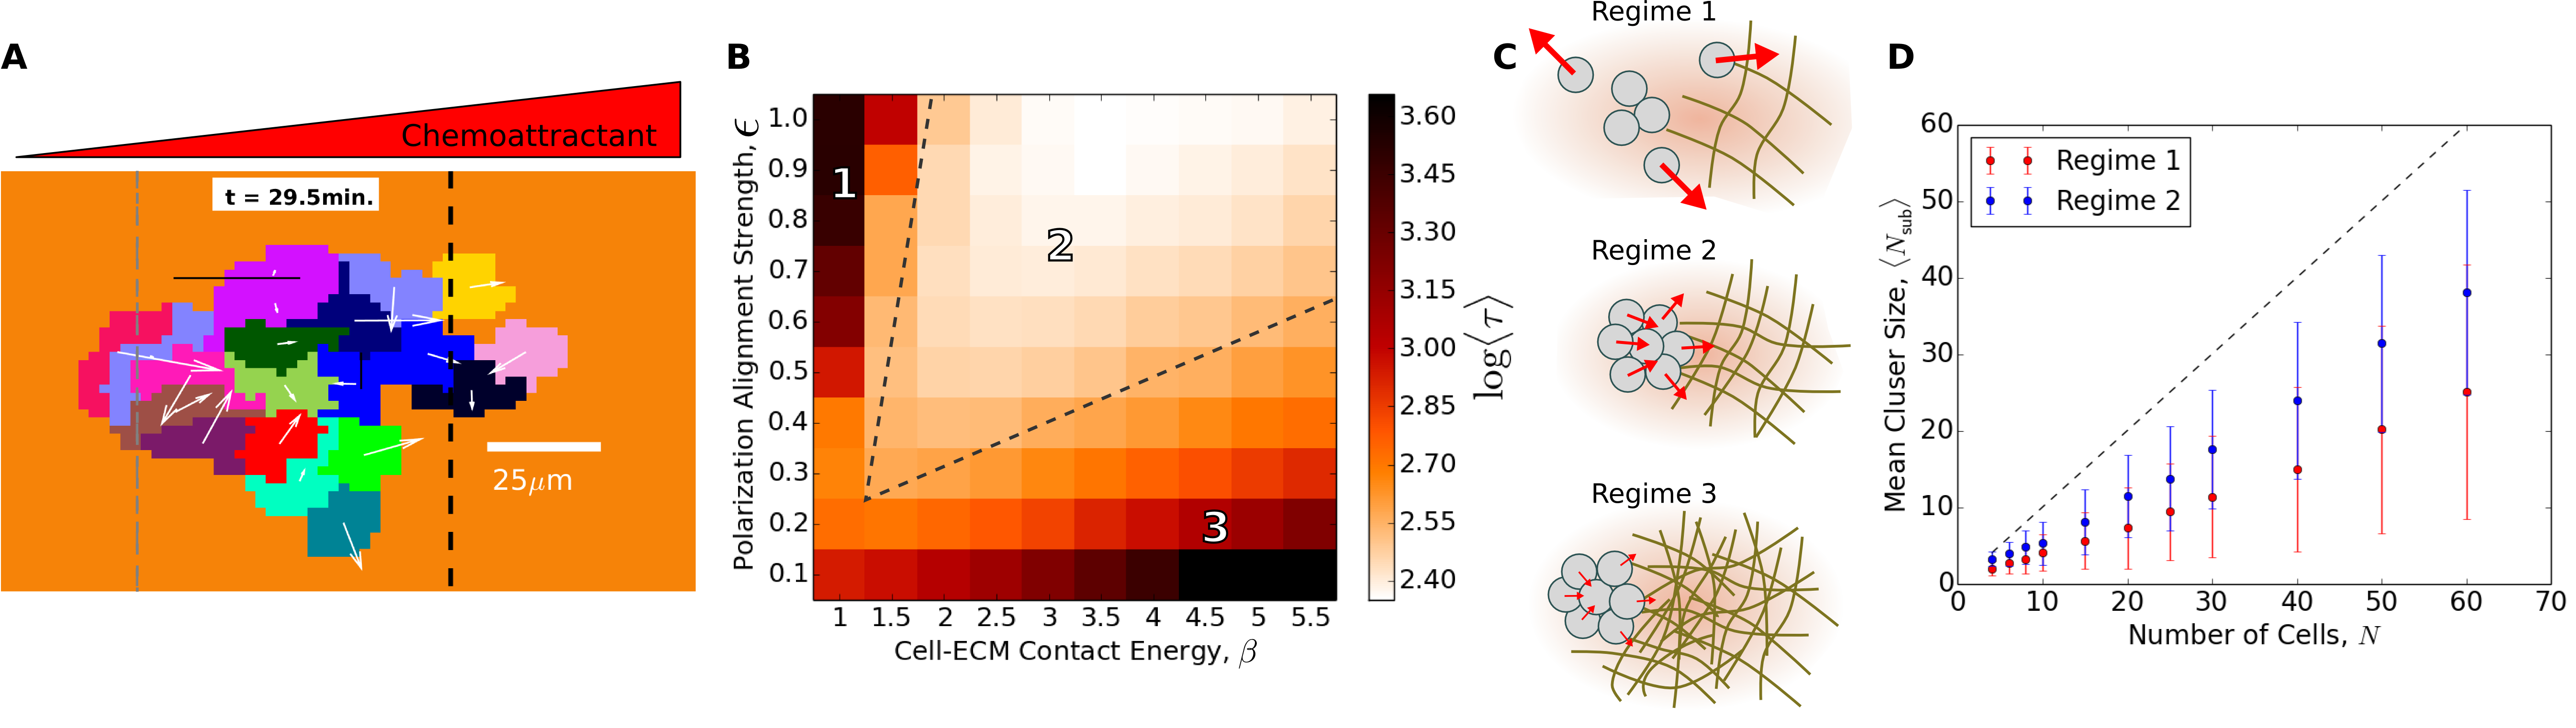
\includegraphics[width=0.90\textwidth]{../fig/ch4_fig2.png}
    \caption{Characterizing the emergent multicellular migration. (A) Snapshot from simulation. Individual cells are distinguished by color and white arrows represent their polarization vectors. The cluster centroid is initially located along the gray dashed line and must cross the black dashed line in order to record a first-passage time event. (B) A heat-map of MFPT in units of minutes as a function of cell-ECM adhesion energy, $\beta$ and polarization bias strength, $\epsilon$. Warmer colors represent higher MFPT values (colorbar). Parameter values for the heat-map: $N = 20$, $\bar{c} = 10\text{nM}$, $g = 0.004\text{nM}/\mu\text{m}$, $\Gamma = 80 (\mu\text{m min.})^{-1}$. Illustrations in (C) represent cluster migratory behavior in their respective regimes of parameter space. Larger values of $\epsilon$ correspond to larger cell polarization vectors (red arrows), whereas larger values of $\beta$ correspond to an ECM that is more difficult to traverse. (D) Mean cluster size
    $\langle N_\text{sub} \rangle$
    as a function of the total number of cells in the system $N$. Regime 1: $\beta = 1.5$, $\epsilon = 1.0$. Regime 2: $\beta = 3.5$, $\epsilon = 0.8$} \label{fig:heat}
\end{figure}


We simulate clusters of various sizes migrating in response to shallow constant chemical gradients over a fixed distance (Fig.\ \ref{fig:heat}A, Movie S1). The simulation results were calibrated using the cluster migration data from Malet-Engra et al.\ \cite{malet2015collective} and assuming a typical cell radius $a = 10 \mu\text{m}$. Similar to the experimental study, initial simulations were conducted with a gradient and background concentration equivalent to $\bar{g} = 0.001 \text{nM}/\mu\text{m}$ and $\bar{c} = 1 \text{nM}$. We found that increasing the gradient and background concentration values to those reported in Table \ref{table:ch4_1} (see pg.\ 11), which still maintain the limit
$a\bar{g} \ll \bar{c}$,
decreased computation cost while yielding the same qualitative results. Therefore all results presented here use the values of $\bar{c}$ and $\bar{g}$ in Table \ref{table:ch4_1}. The simulation timescale was then calibrated such that clusters of cells migrate with velocities on the same order as those in the study by Malet-Engra et al. All simulation parameter values used are presented and motivated in Table \ref{table:ch4_1} unless specified otherwise.

In order to quantify model behavior, statistics on the simulated mean first-passage time (MFPT) for migrating clusters are collected. The first-passage time is the time it takes for the center of mass of a cluster of cells to cross a threshold distance. First it is important to understand the effects of the various parameters in our model on simulations results. Across simulations, two crucial parameters emerge: $\beta$ the cell-ECM adhesion energy, and $\epsilon$ the polarization bias strength. When these two parameters are varied three distinct phases of collective cell migration are clear (regimes 1, 2, and 3 in Fig.\ \ref{fig:heat}B).

Fig.\ \ref{fig:heat}B shows that for sufficiently large $\beta$ the mean first-passage time remains relatively constant as $\beta$ and $\epsilon$ grow in proportion to one another. In this phase, regime 2 of Fig.\ \ref{fig:heat}B, cells migrate as a collective as illustrated in Fig.\ \ref{fig:heat}C. However if the adhesion energy is further increased while the bias strength remains fixed the MFPT starts to increase (regime 3 of Fig.\ \ref{fig:heat}B). This is due to the increased energy cost in cells making protrusions into the ECM. If $\beta$ is increased further the cluster cells will eventually stop moving since protrusions become highly improbable as dictated by the CPM (Fig.\ \ref{fig:heat}C). The other large MFPT phase is due to increasing $\epsilon$
while keeping $\beta$ fixed (regime 1 of Fig.\ \ref{fig:heat}B).
In this case the cell's polarization becomes large enough to overcome the intercell adhesion energy causing the cluster of cells to scatter as illustrated in Fig.\ \ref{fig:heat}C. To further characterize whether a cluster will scatter or remain persistently connected, we track the mean subcluster size $\langle N_\text{sub} \rangle$, defined as the average cluster size weighted by the number of cells present in each constituent cluster (Fig.\ \ref{fig:heat}D). Although cells' initial configuration is that of a single cluster, partial scattering may occur stochastically and reversibly, leading to a value of $\langle N_\text{sub} \rangle$ that is less than the cluster size $N$. As seen in Fig.\ \ref{fig:heat}D, the persistence $\langle N_\text{sub} \rangle/N$ is largely independent of $N$, and clusters in the parameter space of regime 2 are more persistent than those corresponding to regime 1 where cells are likely to scatter permanently. Overall, we see that there is a large region in parameter space which yields physically realistic behavior, and the model breaks down in the limits where we would expect it to. With this in mind we further examine simulations within regime 2 of parameter space.


\begin{figure}[ht]
    \centering
        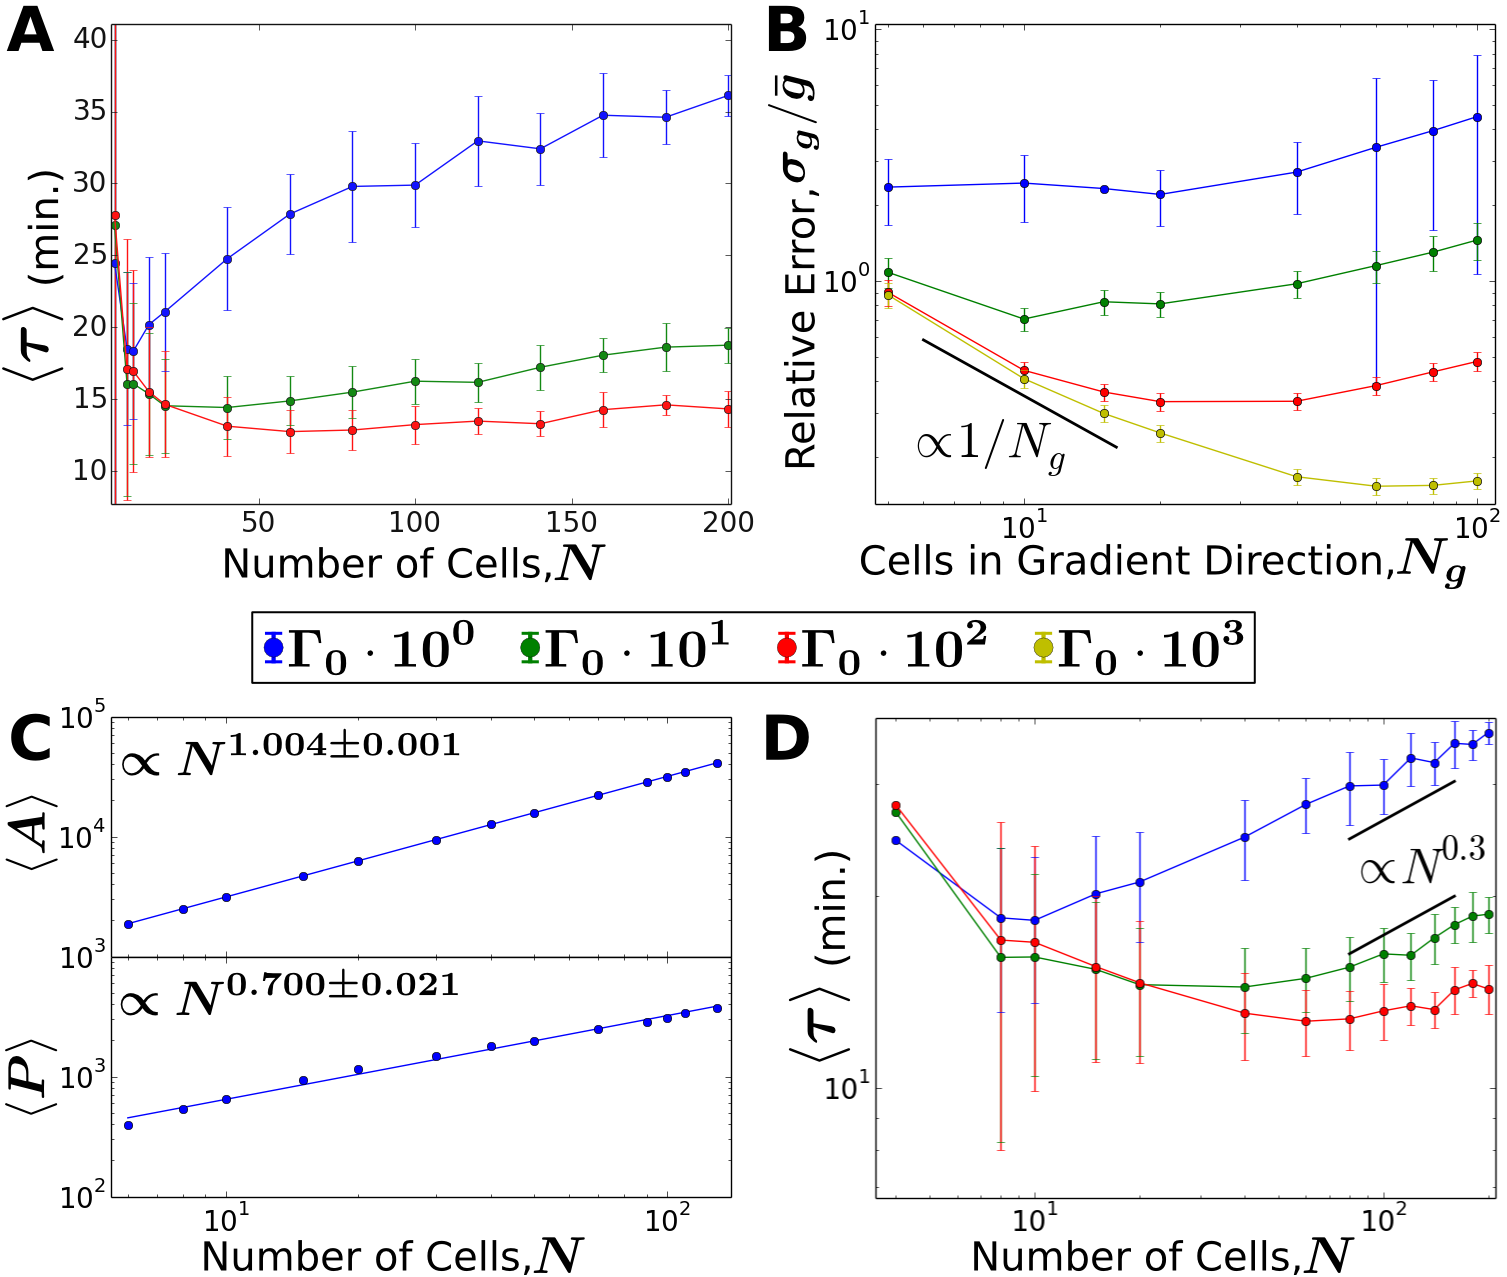
\includegraphics[width=0.80\textwidth]{../fig/ch4_fig3.png}
    \caption{Tradeoff between sensing and drag leads to a minimum mean first-passage time (MFPT) with cluster size. $\Gamma_0 = 0.80 (\mu\text{m} \ \text{min})^{-1}$. (A) MFPT for various values of the exchange rate per unit contact-length $\Gamma$. (B) Relative error in gradient sensing for various values of $\Gamma$. (C) Area $A$ and perimeter $P$ scaling relationships with the number of cells $N$ in a cluster. (D) MFPT results in A on a log-log scale, compared with the geometric prediction arising from C. All error bars represent standard deviation.} \label{fig:results}
\end{figure}


Next we examine the MFPT as a function of cluster size (Fig.\ \ref{fig:results}A). Starting from $N=2$ we see that for sufficiently large $\Gamma$ (red curve), as the number of cells increases the MFPT decreases. This can be understood from our description of multicellular sensing (Eq.\ \ref{eq:G1}): before reaching the critical number of cells in a cluster, the error in gradient sensing decreases as $\sigma_R/\bar{R} \sim N^{-1}$ and so the cluster's ability to more precisely measure the gradient increases. The decreased sensing error translates into more accurately directed cell polarization vectors causing the MFPT to decrease. Fig.\ \ref{fig:results}B shows the relative error vs.\ the number of cells in the cluster that are parallel to the gradient direction, $N_g$. In the small-cluster regime and for fast communication (yellow curve) there is a decrease in relative error with $N_g$, that is in close agreement with the theoretical prediction for the scaling of $N_g^{-1}$
(Eq.\ \ref{eq:G1}). Since the global-reporter exchange rate between cells is very large compared to the degradation rate
($\gamma\gg\mu$)
it is expected that the effects of communication can be neglected as was the case in deriving Eq.\ \ref{eq:G1}. However, as the cluster grows in size the effects of communication can no longer be neglected. As illustrated in Fig.\ \ref{fig:results}B the relative error reaches a lower limit as predicted by Eq.\ \ref{eq:G2} at which sensory precision will no longer increase with increased cluster size.

As the number of cells increases the MFPT tends to saturate to a minimal value and may even begin to increase (Fig.\ \ref{fig:results}A). The MFPT reaches a minimum around $N \sim 10-100$ cells depending on the choice of $\Gamma$, the global molecule exchange rate per unit contact-length. Communication between cells improves as $\Gamma$ increases since more $Y$ molecules can be quickly transmitted between cells, pushing the point of saturation to larger cluster sizes. From these results we see that the model predicts an optimal cluster size for fastest migration. This prediction is in contrast with similar studies which in some cases predict a saturation in velocity and therefore constant MFPT as a function of cluster size \cite{camley2016emergent,malet2015collective}. The dependence of MFPT on cluster size is further explored in the Discussion.

In the limit that $\Gamma a / \mu \lesssim 1$ ($a$ being the cell radius) intercellular communication within the cluster is highly localized, and increasing the size of the cluster will not improve sensory precision. If this is the case then the cluster will have outgrown its optimal size for gradient detection. Instead of the cluster acting as one cohesive gradient-sensing device the cluster will comprise several independent gradient sensors which cannot reliably share information with one another. Therefore, in the small $\Gamma$ limit we expect the MFPT to monotonically increase with increasing $N$ due to increased drag on the cluster. Indeed, simulation results confirm our expectations in the large $N$, small $\Gamma$ limit (Fig.\ \ref{fig:results}A, blue curve).

Next we asked if the MFPT had any dependence on the geometrical properties of the migrating clusters \cite{camley2015collective}. The mean first-passage time should scale proportionally with the drag experienced on the cluster, whereas it should be inversely related to the force driving migration,
\begin{equation} \label{eq:fpt1}
    \langle\tau\rangle \sim \frac{\text{drag}}{\text{force}}.
\end{equation}
The drag on the cluster should scale with the area of the cluster, $\text{drag} \propto A(N)$, and the driving force should scale with the perimeter of the cluster since we know that only cells on the edges of the cluster are polarized in the desired direction, $\text{force} \propto P(N)$. Although the size and shape of clusters will fluctuate we can obtain from many simulations how the average area $\langle A \rangle$ and perimeter $\langle P \rangle$ scale with $N$.
Fig.\ \ref{fig:results}C shows that both scale with powers of $N$, i.e.\ $\langle A \rangle \sim N^d$ and $\langle P \rangle \sim N^f$. We find $d = 1.004 \pm 0.001$, which makes sense since the average area of the should scale linearly with the number of cells. We also find $f = 0.700 \pm 0.021$, which is intriguing because for a circular cluster we would expect $f = 1/2$. The larger value of $f$ reflects the elongated and amoebic shape of the cluster (Fig.\ \ref{fig:heat}A), which causes its perimeter-to-area ratio to be larger than that expected for a circle.

Given these geometric scalings, Eq.\ \ref{eq:fpt1} then makes a prediction: the MFPT should scale as $\langle\tau\rangle \sim N^{d-f} = N^{0.304 \pm 0.021}$. We compare this prediction to the MFPT data, on a log-log scale, in Fig.\ \ref{fig:results}D. We see that in the large $N$, small $\Gamma$ limit, the prediction agrees well with the data (blue and green curves). This demonstrates that the slowdown of large, poorly communicating clusters is dominated by the geometrical aspects of cluster propulsion and drag.

In summary, in the limit that communication between cells is strong ($\Gamma a / \mu \gg 1$), information can be reliably transferred over $n_0 \gg 1$ cells. As long as cluster sizes $N$ remain smaller than $n_0$ cells, there will be an improvement in the sensory capability of the cluster with size, and an associated decrease in the MFPT $\langle\tau\rangle$.  As the critical size $n_0$ is reached, sensory ability will cease to improve with size, and $\langle\tau\rangle$ will reach a minimum. Further addition of cells will cause $\langle\tau\rangle$ to increase according to
$\langle\tau\rangle \sim \text{drag}/\text{force}$, since the drag is proportional to the cluster area, whereas the force is proportional only to the cluster perimeter.


\section{Discussion}

We have developed a model in which collective sensing of noisy chemical gradients induces multicellular migration. The model includes the stochastic processes of ligand diffusion, intercellular communication and cell shape fluctuations.
In the model cells are polarized based on collective gradient information and contact-mediated interactions, leading to biased migration despite the fact that individual cells do not chemotax. We find that the antagonistic effects of sensing and drag result in a minimum mean first-passage time (MFPT) as a function of cluster size, i.e.\ an optimal size for fastest migration. The optimal size is governed by the strength of cell-cell communication, with stronger communication leading to both a larger optimal size and a decreased migration time (Fig.\ \ref{fig:results}D).

Whereas previous models have idealized cell or cluster geometries as perfect circles \cite{ camley2016emergent, camley2015collective}, our use of the cellular Potts model has allowed us to capture natural fluctuations in cell and cluster shape. As a result, we have found that while migrating, clusters adopt a shape that is (i) elongated in the gradient direction and (ii) non-convex (see Fig.\ \ref{fig:heat}A). Both features lead to a cluster perimeter-to-area ratio that is significantly larger than that expected for a circle or other convex shape with aspect ratio near unity. Importantly, we have found that the area and perimeter scalings remain predictive of MFPT in the communication-limited regime (Fig.\ \ref{fig:results}D), even with the observed non-circular and fluctuating geometries.

To the extent possible, our model has been constructed and parameterized using current experiments on collective migration. Intercellular communication is modeled as a direct exchange of messenger molecules between cells since this type of  communication has been implicated in development, organoid branching, angiogenesis, and cancer \cite{ramel2013rab11,ellison2016cell,gerhardt2003vegf,hsu2000cadherin,friedl2009collective}. The chemical concentration and gradient values are selected to ensure that our simulations are in the shallow gradient regime, where experiments show that collectives can respond whereas single cells cannot \cite{ellison2016cell,malet2015collective,rosoff2004new}. Cell size, chemical concentration, chemical gradient, cell-cell contact energy, and cell-ECM contact energy values are taken from previous experimental studies of collective cell behavior (Table \ref{table:ch4_1}).

How do our model predictions compare to experiments? There have been many studies on collective migration \cite{cheung2013collective,puliafito2015three,defranco2008migrating,ramel2013rab11} though only one (to our knowledge), by Malet-Engra et al.\ \cite{malet2015collective}, measures migratory properties as a function of cluster size. The experiments conducted by Malet-Engra et al.\ reveal that beyond a minimum cluster size, the cluster velocity saturates to a maximal value and then remains constant with increasing cluster size. In our study, we find that when communication is strong, the MFPT -- which is inversely related to the mean velocity -- also saturates to a minimal value and remains constant for a large range of cluster sizes. As shown in Fig.\ \ref{fig:results}A (red curve), as the cluster size increases from about 30 to 200 cells the MFPT remains relatively constant, in qualitative agreement with the aforementioned experimental results. This saturation regime occurs when communication is sufficiently strong to suppress, over a large range of cluster sizes, the drag-induced slowdown. Our findings thus suggest that sensory information is reliably transferred throughout the clusters of lymphocytes studied by Malet-Engra et al., and that communication is strong enough that drag does not strongly constrain migration speed for the cluster sizes analyzed.


\begin{figure}[ht]
    \centering
        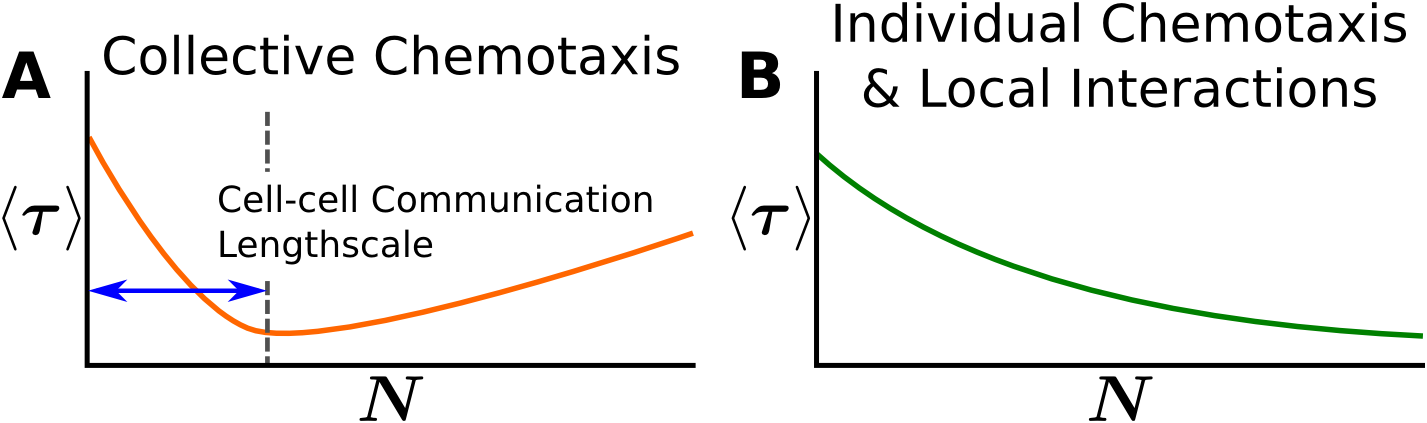
\includegraphics[width=0.80\textwidth]{../fig/ch4_fig4.png}
    \caption{Prediction to distinguish collective from individual chemotaxis in experiments. (A) Expected MFPT behavior for cluster migration driven by collective sensing. (B) Expected MFPT behavior for cluster migration driven by local interactions.} \label{fig:mfpt}
\end{figure}


Furthermore, our results suggest a simple experimental test that can distinguish whether cluster chemotaxis is purely collective or individually driven. Broadly speaking, cluster migration (i) can emerge collectively from cells that communicate, either chemically or mechanically, but do not chemotax alone (as in our model), or (ii) it can result from many individual agents that take independent measurements of the environment and through physical coupling or local interactions produce collective migration \cite{coburn2013tactile,vicsek1995novel} (a so-called ``many wrongs'' mechanism \cite{simons2004many}). As illustrated in Fig.\ \ref{fig:mfpt}A, our results suggest that in the former case, one would observe a minimum in the migration time as a function of the cluster size, with the optimal size determined by the length scale of collective information processing within the cluster. In contrast, as illustrated in Fig.\ \ref{fig:mfpt}B, in the latter case migration is driven by the integrated measurements of many effectively independent agents, and thus one would observe a monotonic decrease in the migration time as a function of the cluster size \cite{simons2004many}. Distinguishing the dependence in Fig.\ \ref{fig:mfpt}A from that in Fig.\ \ref{fig:mfpt}B using microscopy would provide phenomenological evidence of purely collective chemotaxis without relying on molecular-level details.

An important feature of our model and its analysis is that the timescale of sensing is faster than the timescale of cell response and motility (Table \ref{table:ch4_1}). However, in actuality the duration of cells' sensing timescales relative to their response timescales is unknown \cite{ellison2016cell}. If the motility timescale is shorter than that of sensing for a specific cell type than the MFPT dependence on cluster size may be more complicated than predicted. For short response timescales we expect migratory behavior to be more strongly diffusive, but to still remain biased in the direction of the gradient over periods of time larger than the sensing timescale.

In our model, the precision of multicellular migration is determined in part by noise arising from ligand diffusion at the initial sensory stage. As such, the model respects the fundamental limits to the precision of collective gradient sensing set by the physics of diffusion, which were recently tested in collectives of epithelial cells \cite{ellison2016cell, mugler2016limits}. It will be interesting to see how these and similar limits translate from the domain of sensing to that of migration, and whether they depend on the underlying migration mechanism (purely collective, individually driven, or a mixture thereof).



\chapter{Conclusion}

\noindent
Cell chemotaxis is crucial to many biological functions. As discussed in Ch.\ 1, it is critical to growth, nutrient search, development, wound healing, and in several instances, cancer metastasis. Chemotaxis can involve individual cells or collectives migrating in response to chemical concentration gradients. Recently, studies have shown the incredible precision of cell sensing. Detection of shallow gradients that are on the order of a 10 molecule difference across a cell body has been observed. Even more remarkable is that this precision is heightened in cell collectives. Examples from morphogenesis and cancer metastasis demonstrate that collectives can sense gradients an order of magnitude smaller than what's possible for single cells. Although the physical constraints to gradient sensing are well understood and reviewed in Ch.\ 1, how sensing leads to coherent, directed migration remains poorly understood. With this problem in mind, we set out to understand and quantify how the physical limits of chemical sensing lead to constraints on chemotactic performance.

We began by studying the individual chemotaxis of breast cancer cells in Ch.\ 2. In collaboration with Dr.\ Han's research group we used experiments, simulations, and analytical models to place physical constraints on the cells' chemotactic performance. From the simulations we identified the dependence of chemotaxis precision, persistence and speed on crucial environmental parameters like background concentration, gradient, and ECM stiffness. From our analytical approach we found that a biased persistent random walk places bounds on the precision and persistence of the breast cancer cells. In Ch.\ 3, we turned our attention to collective chemotaxis. We developed a novel analytical model that predicts the physical limits of chemotactic precision for two generic classes of collective migration. We found that collective dimensionality is crucial to understanding how correlations between sensory cells cascades to the noise in the collective's perceived gradient direction. Lastly, in Ch.\ 4 we studied an application of the EC class of migration from Ch.\ 3 where communication between cells is explicitly accounted for. Using simulations we test the chemotactic performance of cell collectives in gradients too shallow for single cell detection. Here we again find that chemotactic performance depends on the size of the collective, and it was also shown to depend on the efficacy of intercellular communication.

% Experiments have shown that individual cells as well as collectives are capable of chemotaxis in response to very small chemical signals. From studies on the physical limits to chemical signaling we know that these chemotaxing cells often behave in environments very near these limits, therefore it is important to understand how sensory noise cascades into chemotactic performance. Here in this work we present computational and analytical approaches to attacking these problems. They are important step towards developing a complete predictive model of cell chemotaxis.


%
%  bibliography.tex     June 3, 2002     Mark Senn
%
%  This is the bibliography for a simple, example thesis.
%

% \bibliography{all}
\bibliography{../ref/all}


% Use "\appendix" for one appendix or "\appendices" for more than one
% appendix.
% \appendices
% %
%  revised  demo-citations.tex  2011-09-02  Mark Senn  http://www.ecn.purdue.edu/~mark
%  created  demo-citations.tex  2007-03-21  Mark Senn  http://www.ecn.purdue.edu/~mark
%


\chapter{Demonstrate Citations}

I typed

\begin{verbatim}
    For \LaTeX\ answers I refer to
    % note to self: {\em \LaTeX: A Document Preparation System\/}
    \cite{Lamport:1994}
    and then to
    % note to self: {\em The \LaTeX\ Companion\/}
    \cite{Goossens:1994}
    or
    % note to self: {\em A Guide to LaTeX\/} (1999)
    \cite{Kopka:1999}.
    % note to self: {\em A Guide to LaTeX\/} (1999)
    \cite{Kopka:1999}
    is an updated edition of the 1995 edition
    \cite{Kopka:1995}.
\end{verbatim}

to get

\begin{quotation}
    For \LaTeX\ answers I refer to
    % note to self: {\em \LaTeX: A Document Preparation System\/}
    \cite{Lamport:1994}
    and then to
    % note to self: {\em The \LaTeX\ Companion\/}
    \cite{Goossens:1994}
    or
    % note to self: {\em A Guide to LaTeX\/} (1999)
    \cite{Kopka:1999}.
    % note to self: {\em A Guide to LaTeX\/} (1999)
    \cite{Kopka:1999}
    is an updated edition of the 1995 edition
    \cite{Kopka:1995}.
\end{quotation}

% %
%  demo-figures.tex  2009-10-30  Mark Senn  http://engineering.purdue.edu/~mark
%
%  Demonstrate how to do figures.
%

\chapter{Demonstrate Figures}

The
\verb+h+
specifier used in all the examples below
tells \LaTeX\ to put the figure
``here''
instead of trying
to find a good spot
at the top or bottom of a page.
Specifiers can be combined, for example,
``\verb+\begin{figure}[htbp!]+''.

The complete list of specifiers:

\begin{center}
    \renewcommand{\baselinestretch}{1}\normalsize
    \begin{tabular}{ll}
        \bf Specifier& \bf Description\cr
        \tt b& bottom of page\cr
        \tt h& here on page\cr
        \tt p& on separate page of figures\cr
        \tt t& top of page\cr
        \tt !& try hard to put figure as early as possible\cr
    \end{tabular}
\end{center}

Label ``fi:not-centered'' is ``\ref{fi:not-centered}''.
Label ``sf:four-parts-c'' is ``\ref{sf:four-parts-c}''.

\Repeat{This is the first paragraph.}{5}

\begin{figure}[h]
  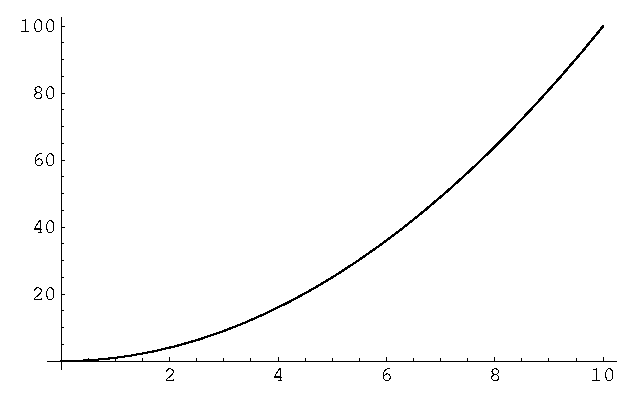
\includegraphics{plot.eps}
  \caption{%
    By default figures are not centered.
    This is a long caption to demonstrate that captions are single spaced.
  }
  \label{fi:not-centered}
\end{figure}

\Repeat{This is the second paragraph.}{10}

\begin{figure}[h]
  \centering
  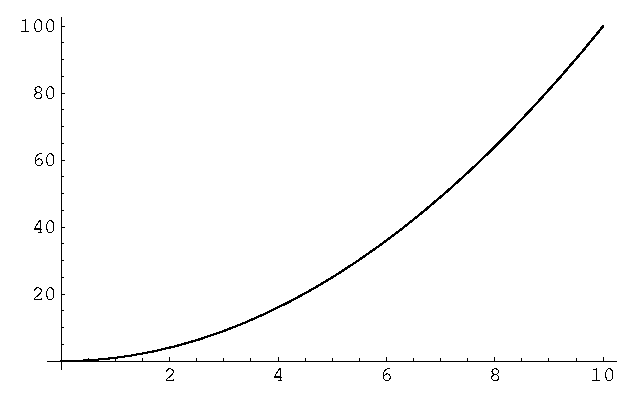
\includegraphics{plot.eps}
  \caption{Use {\tt \char'134centering\/} to center figures.}
  \label{fi:centered}
\end{figure}

\Repeat{This is the third paragraph.}{15}

\begin{figure}[h]
  \centering
  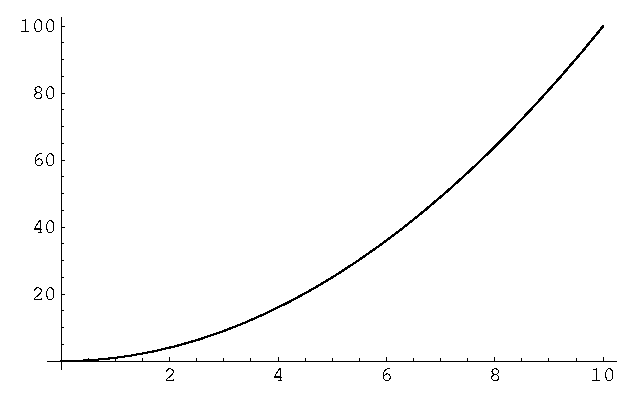
\includegraphics{plot.eps}
  \caption{This is another figuure.}
  \label{fi:another}
\end{figure}

\Repeat{This is the fourth paragraph.}{10}

\begin{figure}[h]
  \centering 
  \subfigure[First subcaption.]{\label{sf:two-parts-a}  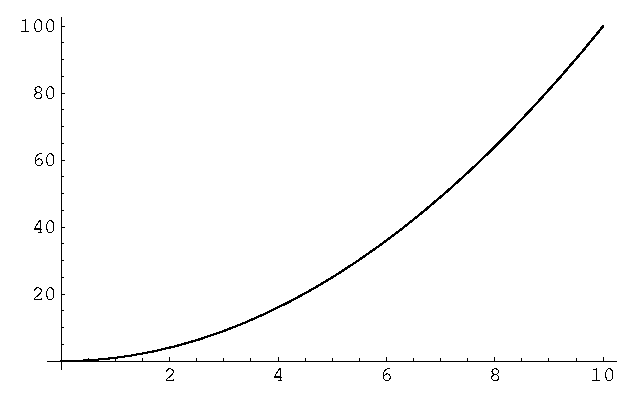
\includegraphics[width=0.3\textwidth]{plot.eps}}%
  \hskip 0.5truein
  \subfigure[Second subcaption.]{\label{sf:two-parts-b}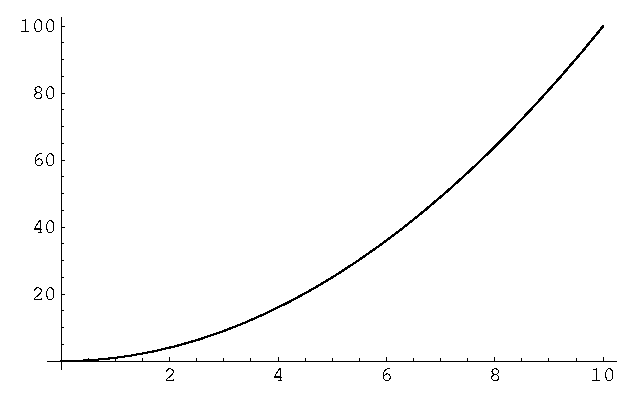
\includegraphics[width=0.3\textwidth]{plot.eps}}
  \caption{This figure has two parts.}
  \label{fi:two-parts}
\end{figure}

\Repeat{This is the fifth paragraph.}{10}

\begin{figure}[h]
  \centering
  \subfigure[First subcaption.]{\label{sf:four-parts-a}  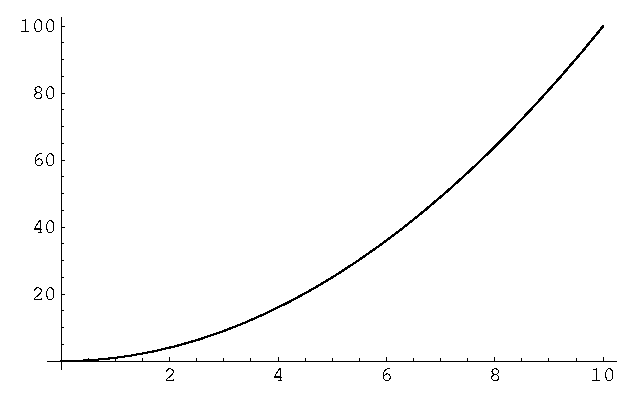
\includegraphics[width=0.3\textwidth]{plot.eps}}%
  \hskip 0.5truein
  \subfigure[Second subcaption.]{\label{sf:four-parts-b}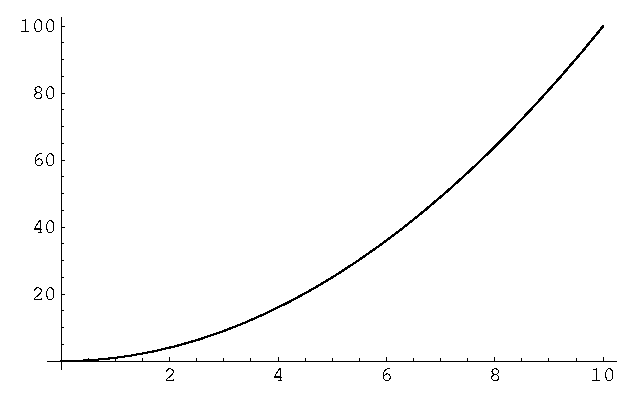
\includegraphics[width=0.3\textwidth]{plot.eps}}
  \subfigure[Third subcaption.]{\label{sf:four-parts-c}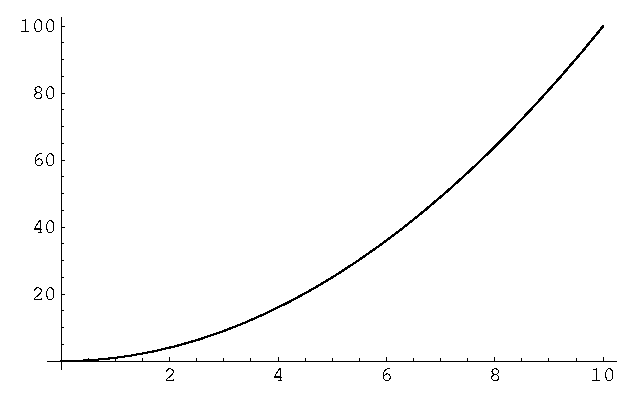
\includegraphics[width=0.3\textwidth]{plot.eps}}%
  \hskip 0.5truein
  \subfigure[Fourth subcaption.]{\label{sf:four-parts-d}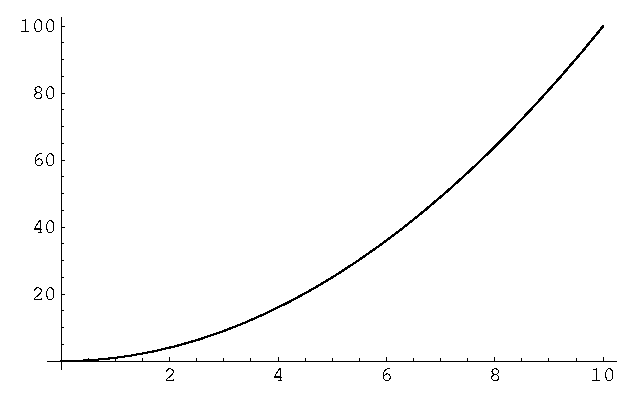
\includegraphics[width=0.3\textwidth]{plot.eps}}
  \caption{This figure has four parts.}
  \label{fi:four-parts}
\end{figure}

\Repeat{This is the sixth paragraph.}{10}

% %
%  THIS FILE DOES SOME UNUSUAL THINGS TO MAKE
%  IT EASIER TO DO DEMONSTRATIONS.  IT SHOULD
%  NOT BE USED AS AN EXAMPLE OF HOW TO PREPARE
%  A FILE.  SEE THE OUTPUT OF THIS FOR LATEX
%  INPUT AND OUTPUT EXAMPLES.
%




%
%  demo-mathematics.tex  2008-12-09  Mark Senn  http://engineering.purdue.edu/~mark
%

\chapter{Demonstrate Mathematics}

    % Use single spacing.
    \Baselinestretch{1}

    % You don't normally need this.
    \mbox{}

    \begin{verbatim}
% From _More Math Into LaTeX_, 4th Edition, page 152:
%     TeX uses $$ to open and close a displayed math environment.
%     In LaTeX, this may occassionally cause problems.  Don't do it.
\[
    E = mc^2
\]
    \end{verbatim}
% From _More Math Into LaTeX_, 4th Edition, page 152:
%     TeX uses $$ to open and close a displayed math environment.
%     In LaTeX, this may occassionally cause problems.  Don't do it.
\[
    E = mc^2
\]
    \vskip\baselineskip
    \hrule
    \vskip0.5\baselineskip
    \filbreak

    \begin{verbatim}
\begin{equation}
    E = mc^2
\end{equation}
    \end{verbatim}
\begin{equation}
    E = mc^2
\end{equation}
    \vskip\baselineskip
    \hrule
    \vskip0.5\baselineskip
    \filbreak

    \begin{verbatim}
% Mydefs.tex defines \be to be \begin{equation} and
% \ee to be \end{equation}.
\be
    E = mc^2
\ee
    \end{verbatim}
% Mydefs.tex defines \be to be \begin{equation} and
% \ee to be \end{equation}.
\be
    E = mc^2
\ee
    \vskip\baselineskip
    \hrule
    \vskip0.5\baselineskip
    \filbreak

    \begin{verbatim}
\be
    x = -\frac{b}{2a} \pm \frac{\sqrt{b^2 - 4ac}}{2a}
\ee
    \end{verbatim}
\be
    x = -\frac{b}{2a} \pm \frac{\sqrt{b^2 - 4ac}}{2a}
\ee
    \vskip\baselineskip
    \hrule
    \vskip0.5\baselineskip
    \filbreak

    \begin{verbatim}
% requires \usepackage{amsmath}; use align* for no equation number
\begin{align}
    a = {}& b + c\\
    x = {}& y + z
\end{align}
    \end{verbatim}
% requires \usepackage{amsmath}; use align* for no equation number
\begin{align}
    a = {}& b + c\\
    x = {}& y + z
\end{align}
    \vskip\baselineskip
    \hrule
    \vskip0.5\baselineskip
    \filbreak

    \begin{verbatim}
\[
    Z = \left(
        \begin{array}{cc}
            a& b\\
            c& d
        \end{array}
    \right)
\]
    \end{verbatim}
\[
    Z = \left(
        \begin{array}{cc}
            a& b\\
            c& d
        \end{array}
    \right)
\]
    \vskip\baselineskip
    \hrule
    \vskip0.5\baselineskip
    \filbreak

    \begin{verbatim}
\begin{equation}
    \begin{split}
        a = {}& b + c\\
            {}& + d + e
    \end{split}      
\end{equation}
    \end{verbatim}
\begin{equation}
    \begin{split}
        a = {}& b + c\\
            {}& + d + e
    \end{split}      
\end{equation}
    \vskip\baselineskip
    \hrule
    \vskip0.5\baselineskip
    \filbreak

    \begin{verbatim}
\be
    (\cos x)^2 + (\sin x)^2 = 1
\ee
    \end{verbatim}
\be
    (\cos x)^2 + (\sin x)^2 = 1
\ee
    \vskip\baselineskip
    \hrule
    \vskip0.5\baselineskip
    \filbreak

    \begin{verbatim}
If $X = \cos x$ and $Y = \sin x$ then $X^2 + Y^2 = 1$.
    \end{verbatim}
If $X = \cos x$ and $Y = \sin x$ then $X^2 + Y^2 = 1$.
    \vskip\baselineskip
    \hrule
    \vskip0.5\baselineskip
    \filbreak

% %
%  demo-multicols.tex  2007-03-19  Mark Senn  http://www.ecn.purdue.edu/~mark
%
%  Demonstrate multicols.
%
%  The multicols package must be loaded for this to work.
%  To load the multicols package put
%      \usepackage{multicols}
%  between the "\documentclass" and "\begin{document}" commands.
%

\chapter{Demonstrate Multicols}

% Put this amount of space between the columns.
\setlength{\columnsep}{0.5truein}

% Separate the columns with a vertical rule this wide.
\setlength{\columnseprule}{0.4pt}

\Repeat{This is one column.}{25}

\begin{multicols}{2}
\Repeat{This is two columns.}{25}
\end{multicols}

\begin{multicols}{3}
\Repeat{This is three columns.}{25}
\end{multicols}

\begin{multicols}{4}
\Repeat{This is four columns.}{25}
\end{multicols}

\begin{multicols}{5}
\Repeat{This is five columns.}{25}
\end{multicols}

% %
%  demo-tables.tex  2014-08-08  Mark Senn
%
%  Demonstrate how to do tables.
%

\chapter{Demonstrate Tables}

% \newlength{\ta}
% \newlength{\tb}
% \newlength{\tc}
% 
% \settowidth{\ta}{\vbox{\hbox{Money}\hbox{Market}}}
% \settowidth{\tb}{\vbox{\hbox{Stocks}\hbox{and}\hbox{Bonds}}}
% \settowidth{\tc}{\vbox{\hbox{Money}\hbox{Market}\hbox{and}\hbox{Stocks}}}
% 
% {
%     \renewcommand{\baselinestretch}{1}
%     \begin{table}
%       \caption{%
%         \hfil Allocation of the IRA and Keogh Wealth\hfil\break
%         \mbox{}\hfil for Investors With or Without Brokerage Accounts\hfil
%       }
%       \label{tab:ira}
%       \begin{center}
%         \begin{tabular}%
%           {%
%             |%
%             c%
%             |%
%             >{\centering\hspace{0pt}}m{\the\ta}%  Money Market
%             |%
%             c%                                    Stocks 
%             |%
%             c%                                    Bonds
%             |%
%             c%                                    Diversified
%             |%
%             >{\centering\hspace{0pt}}m{\the\tb}%  Stocks and Bonds
%             |%
%             >{\centering\hspace{0pt}}m{\the\tc}%  Money Market and Stocks
%             |%
%             c%                                    Others
%             |%
%           }
%           \hline
%           IMP&
%             Money Market&
%             Stocks&
%             Bonds&
%             Diversified&
%             Stocks and Bonds&
%             Money Market and Stocks&
%             Others\tabularnewline
%           \hline
%           1& 14.19\%& 57.71\%& 12.21\%& 4.50\%& 7.36\%& 3.04\%& 0.99\%\tabularnewline \hline
%           2& 14.08\%& 58.18\%& 12.32\%& 4.44\%& 7.30\%& 2.80\%& 0.88\%\tabularnewline \hline
%           3 &14.26\%& 58.09\%& 12.27\%& 4.50\%& 7.19\%& 2.75\%& 0.94\%\tabularnewline \hline
%           4 &13.94\%& 58.11\%& 12.14\%& 4.78\%& 7.35\%& 2.68\%& 0.99\%\tabularnewline \hline
%           5 &13.92\%& 58.13\%& 11.93\%& 4.56\%& 7.60\%& 2.98\%& 0.88\%\tabularnewline \hline
%         \end{tabular}
%       \end{center}
%       This table presents the allocations of the wealth in the IRA
%       and Keogh accounts in various asset classes.
%       Results from each set of imputed data are presented here.
%       The first column lists the number of the imputations,
%       and rest of the columns lists various allocations.
%       Entrees under each asset class show the percentage of investors
%       who have most of their IRA
%       and Keogh wealth invested in that particular asset class.
%       The asset class Diversified
%       includes stocks,
%       bonds,
%       and money market investments.
%       The asset class Others
%       include investments in various life insurance products,
%       annuities,
%       real estate, etc.
%       \medskip
%     \footnotesize SOURCE: Survey of Consumer Finances,
%     2001,
%     Federal Reserve Board,
%     USA.\par
%   \end{table}
% }

Here is a really simple table.

% "h" means put table here---don't let it float to top or bottom of page
\begin{table}[h]
  \caption{American Presidents}
  \begin{center}
    \begin{tabular}{rl}
      \bf Number& \bf Name\\
      1& George Washington\\
      2& John Adams\\
      3& Thomas Jefferson\\
    \end{tabular}
  \end{center}
  \label{ta:American-Presidents}
\end{table}

There are 72.27 points per inch.
I like to put 2 points of vertical space between the heading
(Number Name)
and the first line
(1 George Washington)
of the table.

\begin{table}[h]
  \caption{American Presidents with 2pt vertical space after heading}
  \begin{center}
    \begin{tabular}{rl}
      \bf Number& \bf Name\\[2pt]  % put 2pt vertical space after this line
      1& George Washington\\
      2& John Adams\\
      3& Thomas Jefferson\\
    \end{tabular}
  \end{center}
  \label{ta:American-Presidents-with-2pt}
\end{table}

\LaTeX\ can print horizontal and vertical rules in tables.
I don't like the way this looks.

\begin{table}[h]
  \caption{American Presidents with horizontal and vertical lines}
  \begin{center}
    % "|" prints a vertical rule, "c" means center
    \begin{tabular}{|c|l|}
      % "\hline" prints a horizontal rule
      \hline
      \bf\#& \bf Name\\
      \hline
      1& George Washington\\
      \hline
      2& John Adams\\
      \hline
      3& Thomas Jefferson\\
      \hline
    \end{tabular}
  \end{center}
  \label{ta:American-Presidents-with-horizontal}
\end{table}

\newpage

Here is a more complicated table.

\begin{table}[h]
  \caption{C Bitwise Operators}
  \begin{center}
    % "|" prints a vertical rule, "c" means center
    \begin{tabular}{cccc}
      \bf A& \bf B& \bf A$|$B& \bf A\&B\\[2pt]
      0& 0& 0& 0\\
      0& 1& 1& 0\\
      1& 0& 1& 0\\
      1& 1& 1& 1\\
    \end{tabular}
  \end{center}
  \label{ta:C-Bitwise}
\end{table}

You can use Plain \TeX's \verb+\halign+ command to make tables also.
If you can't do a complicated table using \LaTeX\ commands
you may want to try using Plain \TeX\ commands.
\LaTeX's table making commands use Plain \TeX\ commands.

\begin{table}[h]
  \caption{American Presidents using {\tt\char'134 halign}}
  \hbox to \textwidth{\hss\vbox{\halign{%
    \strut #&      % 0. \strut
    \hfil#\qquad&  % 1. Number
    #\hfil\cr      % 2. Name
    %
    & \bf Number& \bf Name\cr
    \noalign{\vskip 2pt}
    & 1& George Washington\cr
    & 2& John Adams\cr
    & 3& Thomas Jefferson\cr
  }}\hss}
  \label{ta:American-Presidents-using}
\end{table}

The next page shows how to do a table that is too long to fit on one page.

\newpage

% This is loosely based on page 106 of _A Guide to LaTeX_, third edition,
% by Helmut Kopka and Patrick W. Daly.
\begin{longtable}{|l|l|}
    \caption{State Abbreviations}\\
    \hline
    State& Abbreviation\\
    \hline
  \endfirsthead
    \caption[]{\emph{continued}}\\
    \hline
    State& Abbreviation\\
    \hline
  \endhead
    \hline
    \multicolumn{2}{r}{\emph{continued on next page}}
  \endfoot
    \hline
  \endlastfoot
  Alabama& AL\\
  Alaska& AK\\
% American Samoa& AS\\
  Arizona& AZ\\
  Arkansas& AR\\
% Armed Forces Europe& AE\\
% Armed Forces Pacific& AP\\
% Armed Forces the Americas& AA\\
  California& CA\\
  Colorado& CO\\
  Connecticut& CT\\
  Delaware& DE\\
% District of Columbia& DC\\
% Federated States of Micronesia& FM\\
  Florida& FL\\
  Georgia& GA\\
% Guam& GU\\
  Hawaii& HI\\
  Idaho& ID\\
  Illinois& IL\\
  Indiana& IN\\
  Iowa& IA\\
  Kansas& KS\\
  Kentucky& KY\\
  Louisiana& LA\\
  Maine& ME\\
% Marshall Islands& MH\\
  Maryland& MD\\
  Massachusetts& MA\\
  Michigan& MI\\
  Minnesota& MN\\
  Mississippi& MS\\
  Missouri& MO\\
  Montana& MT\\
  Nebraska& NE\\
  Nevada& NV\\
  New Hampshire& NH\\
  New Jersey& NJ\\
  New Mexico& NM\\
  New York& NY\\
  North Carolina& NC\\
  North Dakota& ND\\
% Northern Mariana Islands& MP\\
  Ohio& OH\\
  Oklahoma& OK\\
  Oregon& OR\\
  Pennsylvania& PA\\
% Puerto Rico& PR\\
  Rhode Island& RI\\
  South Carolina& SC\\
  South Dakota& SD\\
  Tennessee& TN\\
  Texas& TX\\
  Utah& UT\\
  Vermont& VT\\
% Virgin Islands& VI\\
  Virginia& VA\\
  Washington& WA\\
  West Virginia& WV\\
  Wisconsin& WI\\
  Wyoming& WY\\
\end{longtable}

\newcommand{\cbackslash}{\char'134}
\newcommand{\copencurly}{\char'173}
\newcommand{\cclosecurly}{\char'175}

\newlength{\twidth}
\newlength{\theight}

\setlength{\twidth}{\textwidth}
\setlength{\theight}{\textheight}

\begin{sidewaystable}
  % The following two lines compensate for what I think is a bug.
  \setlength{\textwidth}{\theight}
  \setlength{\textheight}{\twidth}
  \caption{%
    sidewaystable
    {\tt\cbackslash begin\copencurly tabular\cclosecurly\/}%
    \ldots
    {\tt\cbackslash end\copencurly tabular\cclosecurly\/}%
  }
  \begin{center}
    \begin{tabular}{rl}
      \bf Number& \bf Name\\[2pt]  % put 2pt vertical space after this line
      1& George Washington\\
      2& John Adams\\
      3& Thomas Jefferson\\
    \end{tabular}
  \end{center}
\end{sidewaystable}

\begin{sidewaystable}
  % The following two lines compensate for what I think is a bug.
  \setlength{\textwidth}{\theight}
  \setlength{\textheight}{\twidth}
  \caption{%
    sidewaystable
    {\tt\cbackslash halign\copencurly}\ldots{\tt\cclosecurly\/} table%
  }
  \hbox to \textwidth{\hss\vbox{\halign{%
    \strut #&      % 0. \strut
    \hfil#\qquad&  % 1. Number
    #\hfil\cr      % 2. Name
    %
    & \bf Number& \bf Name\cr
    \noalign{\vskip 2pt}
    & 1& George Washington\cr
    & 2& John Adams\cr
    & 3& Thomas Jefferson\cr
  }}\hss}
\end{sidewaystable}

%\newlength{\ta}
%\settowidth{\ta}{\vbox{\hbox{Money}\hbox{Market}}}
%\newlength{\tb}
%\settowidth{\tb}{\vbox{\hbox{Stocks}\hbox{and}\hbox{Bonds}}}
%\newlength{\tc}
%\settowidth{\tc}{\vbox{\hbox{Money}\hbox{Market}\hbox{and}\hbox{Stocks}}}
%
%  {\renewcommand{\baselinestretch}{1}
%\begin{table}
%  \caption{\hfil Allocation of the IRA and Keogh Wealth\hfil\break\mbox{}\hfil for Investors With or Without Brokerage Accounts\hfil}
%  \label{tab:ira}
%  \begin{center}
%    \begin{tabular}%
%      {%
%        |%
%        c%
%        |%
%        >{\centering\hspace{0pt}}m{\the\ta}%  Money Market
%        |%
%        c%                                    Stocks 
%        |%
%        c%                                    Bonds
%        |%
%        c%                                    Diversified
%        |%
%        >{\centering\hspace{0pt}}m{\the\tb}%  Stocks and Bonds
%        |%
%        >{\centering\hspace{0pt}}m{\the\tc}%  Money Market and Stocks
%        |%
%        c%                                    Others
%        |%
%      }
%      \hline
%      IMP&
%        Money Market&
%        Stocks&
%        Bonds&
%        Diversified&
%        Stocks and Bonds&
%        Money Market and Stocks&
%        Others\tabularnewline
%      \hline
%      1& 14.19\%& 57.71\%& 12.21\%& 4.50\%& 7.36\%& 3.04\%& 0.99\%\tabularnewline \hline
%      2& 14.08\%& 58.18\%& 12.32\%& 4.44\%& 7.30\%& 2.80\%& 0.88\%\tabularnewline \hline
%      3 &14.26\%& 58.09\%& 12.27\%& 4.50\%& 7.19\%& 2.75\%& 0.94\%\tabularnewline \hline
%      4 &13.94\%& 58.11\%& 12.14\%& 4.78\%& 7.35\%& 2.68\%& 0.99\%\tabularnewline \hline
%      5 &13.92\%& 58.13\%& 11.93\%& 4.56\%& 7.60\%& 2.98\%& 0.88\%\tabularnewline \hline
%    \end{tabular}
%  \end{center}
%  This table presents the allocations of the wealth in the IRA
%  and Keogh accounts in various asset classes.
%  Results from each set of imputed data are presented here.
%  The first column lists the number of the imputations,
%  and rest of the columns lists various allocations.
%  Entrees under each asset class show the percentage of investors
%  who have most of their IRA
%  and Keogh wealth invested in that particular asset class.
%  The asset class Diversified
%  includes stocks,
%  bonds,
%  and money market investments.
%  The asset class Others
%  include investments in various life insurance products,
%  annuities,
%  real estate, etc.
%  \medskip
%  \footnotesize SOURCE: Survey of Consumer Finances,
%  2001,
%  Federal Reserve Board,
%  USA.\par
%\end{table}
%  }


% %
%  demo-text.tex  2007-07-17  Mark Senn  http://engineering.purdue.edu/~mark
%

\chapter{Demonstrate Text}

% Use single spacing.
\Baselinestretch{1}

% You don't normally need this.
\mbox{}


%\vbox{
\begin{verbatim}
This is a sentence.
This is a sentence.
This is a sentence.
This is a sentence.
This is a sentence.

This is a sentence.
This is a sentence.
This is a sentence.
This is a sentence.
This is a sentence.
\end{verbatim}
This is a sentence.
This is a sentence.
This is a sentence.
This is a sentence.
This is a sentence.

This is a sentence.
This is a sentence.
This is a sentence.
This is a sentence.
This is a sentence.
\vskip\baselineskip
\hrule
%}
\vskip0.5\baselineskip
\filbreak

%\vbox{
\begin{verbatim}
From \verb+http://www.biblegateway.com/passage/?book_id=1&chapter=1&version=50+:

\begin{quote}
    1 In the beginning God created the heavens and the earth.
    2 The earth was without form,
    and void;
    and darkness was on the face of the deep.
    And the Spirit of God was hovering over the face of the waters.

    3 Then God said,``Let there be light'';
    and there was light.
    4 And God saw the light,
    that it was good;
    and God divided the light from the darkness.
    5 God called the light Day,
    and the darkness He called Night.
    So the evening and the morning were the first day. 
\end{quote}
\end{verbatim}
From \verb+http://www.biblegateway.com/passage/?book_id=1&chapter=1&version=50+:

\begin{quote}
    1 In the beginning God created the heavens and the earth.
    2 The earth was without form,
    and void;
    and darkness was on the face of the deep.
    And the Spirit of God was hovering over the face of the waters.

    3 Then God said,``Let there be light'';
    and there was light.
    4 And God saw the light,
    that it was good;
    and God divided the light from the darkness.
    5 God called the light Day,
    and the darkness He called Night.
    So the evening and the morning were the first day. 
\end{quote}
\vskip\baselineskip
\hrule
%}
\vskip0.5\baselineskip
\filbreak

%\vbox{
\begin{verbatim}
\begin{description}
    \item[apple]
        A red fruit.
    \item[banana]
        A yellow fruit.
        This sentence is to make the entry longer so you can see what happens.
        This sentence is to make the entry longer so you can see what happens.
    \item[cherry]
        A red friut.
\end{description}
\end{verbatim}
\begin{description}
    \item[apple]
        A red fruit.
    \item[banana]
        A yellow fruit.
        This sentence is to make the entry longer so you can see what happens.
        This sentence is to make the entry longer so you can see what happens.
    \item[cherry]
        A red friut.
\end{description}
\vskip\baselineskip
\hrule
%}
\vskip0.5\baselineskip
\filbreak

%\vbox{
\begin{verbatim}
\begin{enumerate}
    \item apple
    \item banana
        This sentence is to make the entry longer so you can see what happens.
        This sentence is to make the entry longer so you can see what happens.
    \item cherry
\end{enumerate}
\end{verbatim}
\begin{enumerate}
    \item apple
    \item banana
        This sentence is to make the entry longer so you can see what happens.
        This sentence is to make the entry longer so you can see what happens.
    \item cherry
\end{enumerate}
\vskip\baselineskip
\hrule
%}
\vskip0.5\baselineskip
\filbreak


%\vbox{
\begin{verbatim}
\begin{itemize}
    \item apple
    \item banana
        This sentence is to make the entry longer so you can see what happens.
        This sentence is to make the entry longer so you can see what happens.
    \item cherry
\end{itemize}
\end{verbatim}
\begin{itemize}
    \item apple
    \item banana
        This sentence is to make the entry longer so you can see what happens.
        This sentence is to make the entry longer so you can see what happens.
    \item cherry
\end{itemize}
\vskip\baselineskip
\hrule
%}
\vskip0.5\baselineskip
\filbreak


% A vita is optional for masters theses
% and required for doctoral dissertations.
% Reference: TM2006 page 13.
% CHANGE NEXT LINE?
% %
%  vita.tex   2003.07.23  14:59:33   Mark Senn <mds@purdue.edu>
%
%  This is the vita for a simple, example thesis.
%
%  A vita is required only in a doctoral dissertation.
%

\begin{vita}
    [Put a brief autobiographical sketch here.]
\end{vita}


\end{document}
